% This is the Reed College LaTeX thesis template. Most of the work
% for the document class was done by Sam Noble (SN), as well as this
% template. Later comments etc. by Ben Salzberg (BTS). Additional
% restructuring and APA support by Jess Youngberg (JY).
% Your comments and suggestions are more than welcome; please email
% them to cus@reed.edu
%
% See https://www.reed.edu/cis/help/LaTeX/index.html for help. There are a
% great bunch of help pages there, with notes on
% getting started, bibtex, etc. Go there and read it if you're not
% already familiar with LaTeX.
%
% Any line that starts with a percent symbol is a comment.
% They won't show up in the document, and are useful for notes
% to yourself and explaining commands.
% Commenting also removes a line from the document;
% very handy for troubleshooting problems. -BTS

% As far as I know, this follows the requirements laid out in
% the 2002-2003 Senior Handbook. Ask a librarian to check the
% document before binding. -SN

%%
%% Preamble
%%
% \documentclass{<something>} must begin each LaTeX document
\documentclass[12pt,twoside]{reedthesis}
% Packages are extensions to the basic LaTeX functions. Whatever you
% want to typeset, there is probably a package out there for it.
% Chemistry (chemtex), screenplays, you name it.
% Check out CTAN to see: https://www.ctan.org/
%%
\usepackage{graphicx,latexsym}
\usepackage{subcaption}
\usepackage{amsmath}
\usepackage{amssymb,amsthm}
\usepackage{longtable,booktabs,setspace}
\usepackage{chemarr} %% Useful for one reaction arrow, useless if you're not a chem major
\usepackage[hyphens]{url}
% Added by CII
\usepackage{hyperref}
\usepackage{lmodern}
\usepackage{float}
\floatplacement{figure}{H}
% Thanks, @Xyv
\usepackage{calc}
% End of CII addition
\usepackage{rotating}

% Next line commented out by CII
%%% \usepackage{natbib}
% Comment out the natbib line above and uncomment the following two lines to use the new
% biblatex-chicago style, for Chicago A. Also make some changes at the end where the
% bibliography is included.
%\usepackage{biblatex-chicago}
%\bibliography{thesis}


% Added by CII (Thanks, Hadley!)
% Use ref for internal links
\renewcommand{\hyperref}[2][???]{\autoref{#1}}
\def\chapterautorefname{Chapter}
\def\sectionautorefname{Section}
\def\subsectionautorefname{Subsection}
% End of CII addition

% Added by CII
\usepackage{caption}
\captionsetup{width=5in}
% End of CII addition

% \usepackage{times} % other fonts are available like times, bookman, charter, palatino

% Syntax highlighting #22
  \usepackage{color}
  \usepackage{fancyvrb}
  \newcommand{\VerbBar}{|}
  \newcommand{\VERB}{\Verb[commandchars=\\\{\}]}
  \DefineVerbatimEnvironment{Highlighting}{Verbatim}{commandchars=\\\{\}}
  % Add ',fontsize=\small' for more characters per line
  \usepackage{framed}
  \definecolor{shadecolor}{RGB}{248,248,248}
  \newenvironment{Shaded}{\begin{snugshade}}{\end{snugshade}}
  \newcommand{\AlertTok}[1]{\textcolor[rgb]{0.94,0.16,0.16}{#1}}
  \newcommand{\AnnotationTok}[1]{\textcolor[rgb]{0.56,0.35,0.01}{\textbf{\textit{#1}}}}
  \newcommand{\AttributeTok}[1]{\textcolor[rgb]{0.77,0.63,0.00}{#1}}
  \newcommand{\BaseNTok}[1]{\textcolor[rgb]{0.00,0.00,0.81}{#1}}
  \newcommand{\BuiltInTok}[1]{#1}
  \newcommand{\CharTok}[1]{\textcolor[rgb]{0.31,0.60,0.02}{#1}}
  \newcommand{\CommentTok}[1]{\textcolor[rgb]{0.56,0.35,0.01}{\textit{#1}}}
  \newcommand{\CommentVarTok}[1]{\textcolor[rgb]{0.56,0.35,0.01}{\textbf{\textit{#1}}}}
  \newcommand{\ConstantTok}[1]{\textcolor[rgb]{0.00,0.00,0.00}{#1}}
  \newcommand{\ControlFlowTok}[1]{\textcolor[rgb]{0.13,0.29,0.53}{\textbf{#1}}}
  \newcommand{\DataTypeTok}[1]{\textcolor[rgb]{0.13,0.29,0.53}{#1}}
  \newcommand{\DecValTok}[1]{\textcolor[rgb]{0.00,0.00,0.81}{#1}}
  \newcommand{\DocumentationTok}[1]{\textcolor[rgb]{0.56,0.35,0.01}{\textbf{\textit{#1}}}}
  \newcommand{\ErrorTok}[1]{\textcolor[rgb]{0.64,0.00,0.00}{\textbf{#1}}}
  \newcommand{\ExtensionTok}[1]{#1}
  \newcommand{\FloatTok}[1]{\textcolor[rgb]{0.00,0.00,0.81}{#1}}
  \newcommand{\FunctionTok}[1]{\textcolor[rgb]{0.00,0.00,0.00}{#1}}
  \newcommand{\ImportTok}[1]{#1}
  \newcommand{\InformationTok}[1]{\textcolor[rgb]{0.56,0.35,0.01}{\textbf{\textit{#1}}}}
  \newcommand{\KeywordTok}[1]{\textcolor[rgb]{0.13,0.29,0.53}{\textbf{#1}}}
  \newcommand{\NormalTok}[1]{#1}
  \newcommand{\OperatorTok}[1]{\textcolor[rgb]{0.81,0.36,0.00}{\textbf{#1}}}
  \newcommand{\OtherTok}[1]{\textcolor[rgb]{0.56,0.35,0.01}{#1}}
  \newcommand{\PreprocessorTok}[1]{\textcolor[rgb]{0.56,0.35,0.01}{\textit{#1}}}
  \newcommand{\RegionMarkerTok}[1]{#1}
  \newcommand{\SpecialCharTok}[1]{\textcolor[rgb]{0.00,0.00,0.00}{#1}}
  \newcommand{\SpecialStringTok}[1]{\textcolor[rgb]{0.31,0.60,0.02}{#1}}
  \newcommand{\StringTok}[1]{\textcolor[rgb]{0.31,0.60,0.02}{#1}}
  \newcommand{\VariableTok}[1]{\textcolor[rgb]{0.00,0.00,0.00}{#1}}
  \newcommand{\VerbatimStringTok}[1]{\textcolor[rgb]{0.31,0.60,0.02}{#1}}
  \newcommand{\WarningTok}[1]{\textcolor[rgb]{0.56,0.35,0.01}{\textbf{\textit{#1}}}}

% To pass between YAML and LaTeX the dollar signs are added by CII
\title{Addressing The Scientific Reproducibility Crisis Through Educational Software Integration}
\author{Audrey M. Bertin}
% The month and year that you submit your FINAL draft TO THE LIBRARY (May or December)
\date{May 2021}
\division{Statistical and Data Sciences}
\advisor{Benjamin S. Baumer}
\institution{Smith College}
\degree{Bachelor of Arts}
%If you have two advisors for some reason, you can use the following
% Uncommented out by CII
\altadvisor{Albert Y. Kim}
% End of CII addition

%%% Remember to use the correct department!
\department{Statistical and Data Sciences}
% if you're writing a thesis in an interdisciplinary major,
% uncomment the line below and change the text as appropriate.
% check the Senior Handbook if unsure.
%\thedivisionof{The Established Interdisciplinary Committee for}
% if you want the approval page to say "Approved for the Committee",
% uncomment the next line
%\approvedforthe{Committee}

% Added by CII
%%% Copied from knitr
%% maxwidth is the original width if it's less than linewidth
%% otherwise use linewidth (to make sure the graphics do not exceed the margin)
\makeatletter
\def\maxwidth{ %
  \ifdim\Gin@nat@width>\linewidth
    \linewidth
  \else
    \Gin@nat@width
  \fi
}
\makeatother

%Added by @MyKo101, code provided by @GerbrichFerdinands
\newlength{\cslhangindent}
\setlength{\cslhangindent}{1.5em}
\newenvironment{CSLReferences}%
  {}%
  {\par}

\renewcommand{\contentsname}{Table of Contents}
% End of CII addition

\setlength{\parskip}{0pt}

% Added by CII

\providecommand{\tightlist}{%
  \setlength{\itemsep}{0pt}\setlength{\parskip}{0pt}}

\Acknowledgements{
This project would not have been possible without the guidance of Professor Ben Baumer, who helped inspire my interest in data science and mentored me throughout this project for the last two years.
I would also like to extend my thanks to Jenny Bryan and Hadley Wickham, whose advice has helped guide the development of several features in \texttt{fertile}, along with the authors of all of the R packages utilized by \texttt{fertile} to achieve its functionality.
Additionally, a huge thanks to the many introductory data science students who volunteered their time as part of a study to test the effectiveness of implementing \texttt{fertile} in the classroom. The help of all these Smithies was invaluable in ensuring that the overall \texttt{fertile} product was as user friendly and effective as possible.
}

\Dedication{

}

\Preface{

}

\Abstract{
Data science research is considered \emph{reproducible} when the associated code and data files produce identical results when run by another analyst. Although reproducibility is a key component in the advancement of scientific knowledge, a significant proportion of research articles and other analyses fail to meet reproducibility standards. Steps have been taken to address this issue, including academic courses on reproducibility, additional requirements or recommendations for journal article acceptance, and a variety of software tools. However, many of these are challenging to use, are too generalized, or are not accessible to a wide audience. In this thesis, I present my work on developing \texttt{fertile}, an \texttt{R} package designed to help improve the reproducibility of \texttt{R\ Projects} and address the limitations of other solutions by being 1) simple to use, 2) easily accessible, 2) broad in scope, 3) tailored to the specific challenges faced by R users, 4) customizable, and 5) educational. Chapter 1 considers the background information motivating \texttt{fertile}, including explanation of reproducibility, its issues, current solutions, and their limitations. Chapter 2 is code-focused, demonstrating the functions available in \texttt{fertile} to address different aspects of reproducibility and delving into some of the details of how the software works. Finally, Chapter 3 considers \texttt{fertile}'s potential applications in the real world, including an in-depth analysis of an experiment involving \texttt{fertile}'s integration into an introductory data science course at Smith College.
}

	\usepackage{booktabs}
 \usepackage{longtable}
 \usepackage{array}
 \usepackage{multirow}
 \usepackage{wrapfig}
 \usepackage{float}
 \usepackage{colortbl}
 \usepackage{pdflscape}
 \usepackage{tabu}
 \usepackage{threeparttable}
 \usepackage{threeparttablex}
 \usepackage[normalem]{ulem}
 \usepackage{makecell}
 \usepackage{xcolor}
% End of CII addition
%%
%% End Preamble
%%
%
\begin{document}

% Everything below added by CII
  \maketitle

\frontmatter % this stuff will be roman-numbered
\pagestyle{empty} % this removes page numbers from the frontmatter
  \begin{acknowledgements}
    This project would not have been possible without the guidance of Professor Ben Baumer, who helped inspire my interest in data science and mentored me throughout this project for the last two years.
    I would also like to extend my thanks to Jenny Bryan and Hadley Wickham, whose advice has helped guide the development of several features in \texttt{fertile}, along with the authors of all of the R packages utilized by \texttt{fertile} to achieve its functionality.
    Additionally, a huge thanks to the many introductory data science students who volunteered their time as part of a study to test the effectiveness of implementing \texttt{fertile} in the classroom. The help of all these Smithies was invaluable in ensuring that the overall \texttt{fertile} product was as user friendly and effective as possible.
  \end{acknowledgements}

  \hypersetup{linkcolor=black}
  \setcounter{secnumdepth}{2}
  \setcounter{tocdepth}{2}
  \tableofcontents


  \listoffigures
  \begin{abstract}
    Data science research is considered \emph{reproducible} when the associated code and data files produce identical results when run by another analyst. Although reproducibility is a key component in the advancement of scientific knowledge, a significant proportion of research articles and other analyses fail to meet reproducibility standards. Steps have been taken to address this issue, including academic courses on reproducibility, additional requirements or recommendations for journal article acceptance, and a variety of software tools. However, many of these are challenging to use, are too generalized, or are not accessible to a wide audience. In this thesis, I present my work on developing \texttt{fertile}, an \texttt{R} package designed to help improve the reproducibility of \texttt{R\ Projects} and address the limitations of other solutions by being 1) simple to use, 2) easily accessible, 2) broad in scope, 3) tailored to the specific challenges faced by R users, 4) customizable, and 5) educational. Chapter 1 considers the background information motivating \texttt{fertile}, including explanation of reproducibility, its issues, current solutions, and their limitations. Chapter 2 is code-focused, demonstrating the functions available in \texttt{fertile} to address different aspects of reproducibility and delving into some of the details of how the software works. Finally, Chapter 3 considers \texttt{fertile}'s potential applications in the real world, including an in-depth analysis of an experiment involving \texttt{fertile}'s integration into an introductory data science course at Smith College.
  \end{abstract}

\mainmatter % here the regular arabic numbering starts
\pagestyle{fancyplain} % turns page numbering back on

\hypertarget{prologue}{%
\chapter*{Prologue}\label{prologue}}
\addcontentsline{toc}{chapter}{Prologue}

If it weren't for Professor Ben Baumer, I would not be here writing this thesis today. The Introduction to Data Science course I took with him in my first semester at Smith College spurred on my love for the field, prompting me to declare a major---with Ben as my adviser---soon after.

That course---SDS 192---was my first introduction to the topic of scientific reproducibility. In Ben's class, one of the first undergraduate courses in the country to implement reproducibility as part of the curriculum (Baumer, Cetinkaya-Rundel, Bray, Loi, \& Horton (2014)), I was introduced to a variety of tools that could help make my work more reproducible. I learned how to write effective narrative reports with RMarkdown, how to implement version control on GitHub, how to write well-styled code, and how to use R projects to structure my files in a way that was easy to manage.

Through this work, I began to see the benefits of emphasizing a reproducible workflow. When I worked on projects with other students, the tools I learned in class enabled us to collaborate with one another easily and keep track of the progress we had made. And when I tried to look back at my own work from the past, my attention to reproducibility meant that it was much easier for me to re-compute and understand what I had done previously.

Additionally, my work in Introduction to Data Science helped build a strong interest in R. I developed a love for programming in the language and was curious to learn more about how it worked---both behind the scenes and practice. This interest prompted me to pursue research in the field. I wanted to expand my knowledge and challenge myself by learning about and solving cutting-edge issues in the data science domain.

As soon as I felt that I had built up enough coding experience to be able to tackle challenging issues, I reached out to the data science faculty to see if there were any opportunities. Ben enthusiastically welcomed me in, telling me that he had recently started developing an R package focused on reproducibility and offering me a position assisting him with writing it. That was when I first learned about \texttt{fertile}.

As part of his interest in reproducibility, Ben had been working---with help from Hadley Wickham and Jenny Bryan of RStudio---to develop a package designed to help users create optimal conditions for reproducible work in R (titled ``fertile'').

When it was presented to me, the package was incomplete. Several of the major functions that exist now were there at the time, but there were not many features beyond the basics. Additionally, several functions were not fully written or were throwing errors, the package had little to no documentation, and the majority of tests that had been written to test the functions were failing.

I was given the opportunity to join the project and help move \texttt{fertile} to a functional state: to fix the errors that were present, document the package, and write new functions to expand the operation beyond the barebones structure that was present.

The \texttt{fertile} project was an excellent fit for me. The package was not yet in a functional state, but had an excellent base of code to work off of. Given that it already had some basic functions and a strong structure, \texttt{fertile} provided a perfect opportunity for me to learn about the process of writing R packages.

The more I worked on \texttt{fertile}, the more interested in the project I became. The package was unlike anything else I had been exposed to in data science. Most of my course work had been in the form of front-end coding: conducting data analyses and visualizing information. \texttt{fertile} is nothing like that. It operates completely behind the scenes, conducting a kind of meta-analysis to determine the reproducibility of a data science project. Rather than writing code to analyze data, I had to learn how to write code to analyze code that \emph{other people} wrote to analyze data.

This was a complex problem. It involved capturing information about the user's file system and their RStudio environment, both of which I knew nothing about. It also involved tracking and recording user behavior---something definitely not taught in data analysis courses. Even experienced R users deemed some of the goals associated with the package to be lofty. On the question of whether it was possible to test whether R code contained uncontrolled randomness, one coder said it was ``probably impossible,'' while another said there was ``fundamentally no way'' to achieve it (see \url{https://stackoverflow.com/questions/43638773/comprehensive-way-to-check-for-functions-that-use-the-random-number-generator-in}).

The challenge of the problems at hand, however, was what made them interesting. Most of the time, there was no way to use my past coding knowledge to solve them---rather, I had to research and test out new solutions. While the process was at times frustrating, particularly given that some of the errors I came across had likely never been seen by any other R user, it was an incredible learning opportunity. I was exposed to a wide variety of R features I would likely have never seen otherwise and greatly broadened my problem-solving and troubleshooting skills.

Every problem I solved made me more confident in my abilities and more excited to work on the \texttt{fertile}. I delved more into the topic of reproducibility and looked at some of the work by other researchers and code developers. This research introduced me to new aspects of reproducibility I wanted to include in the package and inspired me to expand its scope.

This thesis is the culmination of the work I have been doing with \texttt{fertile} for the past two years.

\hypertarget{reproducibility}{%
\chapter{An Introduction to Reproducibility}\label{reproducibility}}

\hypertarget{what-is-reproducibility}{%
\section{What Is Reproducibility?}\label{what-is-reproducibility}}

Research in the field of data science is considered fully \emph{reproducible} when the relevant code and data files produce identical results when run by another analyst, or more generally, when a researcher can ``duplicate the results of a prior study using the same materials as were used by the original investigator'' (Bollen, Cacioppo, Krosnick, Olds, \& Dean (2015)).

This term was first coined in 1992 by computer scientist Jon Claerbout, who associated it with a ``software platform and set of procedures that permit the reader of a paper to see the entire processing trail from the raw data and code to figures and tables'' (Claerbout \& Karrenbach (1992)).

Since its inception, the concept of reproducibility has been applied across many different data-intensive fields, including epidemiology, computational biology, economics, clinical trials, and, now, the more general domain of statistical and data sciences (Goodman, Fanelli, \& Ioannidis (2016)).

There are many benefits to reproducibility in scientific research. When researchers share their work in a reproducible format, readers can much more easily determine the accuracy of any findings by following the steps from raw data to conclusions. The creators of reproducible work can also more easily receive more specific feedback on their work, by allowing others to look through their process and even attempt pieces of the work themselves. Moreover, reproducibility makes it much simpler to pass on knowledge. Others interested in the same research topic as in a published work can review the associated code and/or data and then apply some of the the methods and ideas to their own work.

Although often confused, the concept of \emph{reproducibility} is distinct from the related idea of \emph{replicability}: the ability of a researcher to duplicate the results of a study when following the original procedure but collecting new data. Replicability has larger-scale implications than reproducibility; the findings of research studies can not be accepted unless a variety of other researchers come to the same conclusions through independent work.
\begin{figure}

{\centering 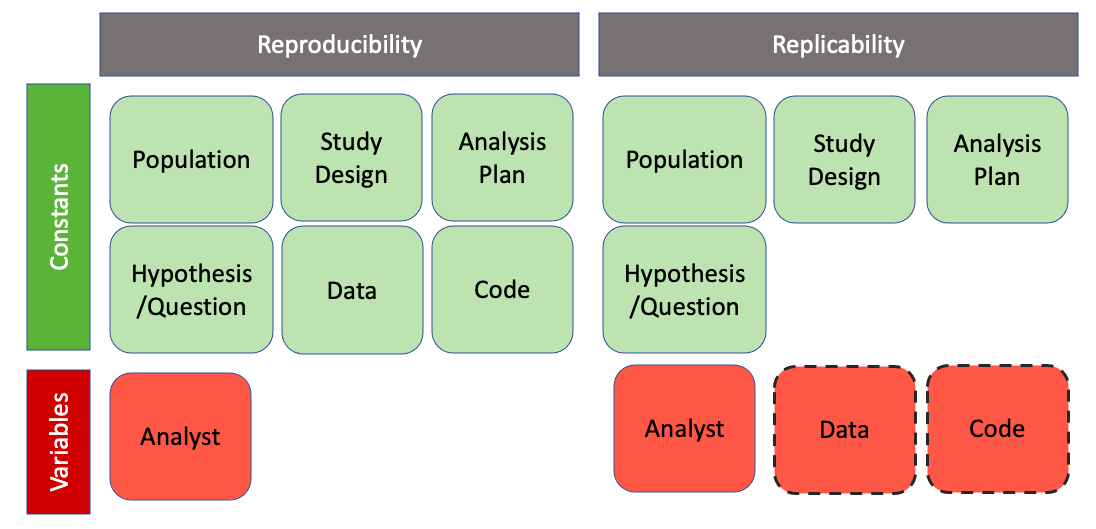
\includegraphics[width=1\linewidth]{figure/versus} 

}

\caption{Reproducibility vs. Replicability --- In reproducibility, data and code remain constant, while in replicability they are variable.}\label{fig:unnamed-chunk-3}
\end{figure}
Reproducibility and replicability are both necessary to the advancement of scientific research, but they vary significantly in terms of their difficulty to achieve. Reproducibility, in theory, is somewhat simple to attain in data analyses--because code is inherently non-random (excepting applications involving random number generation) and data remain consistent, variability is highly restricted. The achievement of replicability, on the other hand, is a much more complex challenge, involving significantly more variablility and requiring high quality data, effective study design, and robust hypotheses.

\hypertarget{the-reproducibility-crisis}{%
\section{The Reproducibility Crisis}\label{the-reproducibility-crisis}}

Despite the apparent simplicity of achieving reproducibility, a significant proportion of the work produced in the scientific community fails to meet reproducibility standards. 52\% of respondents in a 2016 Nature survey believed that science was going through a ``significant crisis'' of reproducibility, while an additional 38\% recognized a ``slight crisis.'' Additionally, the vast majority of researchers across all fields studied reported having been unable to reproduce another researcher's results, while approximately half reported having been unable to reproduce their own (Baker (2016)). Other studies paint an even bleaker picture: Baker (2015) found that over 50\% of studies psychology failed reproducibility tests and Begley \& Ellis (2012) found that figure closer to 90\% in the field of cancer biology.

In the past several years, this ``crisis'' of reproducibility has risen toward the forefront of scientific discussion. Without reproducibility, the scientific community cannot properly verify study results. This makes it difficult to identify which information should be believed and which should not, and increases the likelihood that studies sharing misleading information will be dispersed. The rise of data-driven technologies, alongside our newfound ability to instantly share knowledge worldwide, has made reproducibility increasingly critical to the advancement of scientific understanding, necessitating the development of solutions for addressing the issue.

Academics have recognized this, and publications on the topic appear to have increased significantly in the last several years. For example:
\begin{enumerate}
\def\labelenumi{\arabic{enumi}.}
\item
  Eisner (2018) writes that much of science cannot be reproduced, arguing that some of the major factors behind the problem are fraud, encouraged by the need to publish in top journals, poor experimental design, and poor statistical analysis.
\item
  Fidler \& Wilcox (2018) argue that the term ``reproducibility crisis'' has gained significant currency over the last decade after many large-scale reproducibility studies---including the \emph{Nature} study discussed previously---have returned negative results.
\item
  Gosselin (2019) shares a call to action (summarized by the acronym ACTS---\textbf{AC}cess to \textbf{T}ransparent \textbf{S}tatistics), assembling measures that can be implemented by journals to increase the quality of statistical publications: standardizing paragraph contents, requiring a paragraph on statistical limitations, providing funding to study reproducibility, and requiring that methods sections start with statistics.
\item
  McArthur (2019) argues that a common theme in the issue of reproducibility and related challenges is the ``increasing demands of complex research requiring use of multiple experimental and computational research methods'' and promises to take steps to improve reproducibility in the \emph{Biointerphase} journal.
\item
  Wallach, Boyack, \& Ioannidis (2018) survey a random sample of biomedical journal articles in order to analyze their data availability for the purposes of reproducibility. They find results that are somewhat more positive than previous studies---indicating that perhaps the biomedical sciences are moving in the right direction---but argue that there is still a long way to go before true journal reproducibility is achieved.
\end{enumerate}
\hypertarget{the-components-of-reproducible-research}{%
\section{The Components of Reproducible Research}\label{the-components-of-reproducible-research}}

In order to see why there is an issue with reproducibility and gain a sense of how to solve it, it is important to first understand the components of reproducibility. ``What parts does researcher need to include, or what steps do they need to take, to be able to declare their work reproducible?''

Publications attempting to answer this question can be found across a variety of fields. However, as Goodman, Fanelli, \& Ioannidis (2016) argue, both the framework and terms used to describe reproducibility vary significantly across the sciences, and the scientific community has been unable to agree upon universally applicable clear standards.

At a minimum, according to Goodman, Fanelli, \& Ioannidis (2016), achieving reproducibility requires the sharing of data (either raw or processed), relevant metadata, code, and related software. However, according to others, the full achievement of reproducibility may require additional components.

Kitzes, Turek, \& Deniz (2017) present a series of case studies on reproducibility practices from across the data-intensive sciences, illustrating many different recommendations and techniques for achieving reproducibility. Although their work does not come to a consensus on the exact standards of reproducibility that should be followed, several common trends and principles emerge from their analysis that extend beyond the minimum recommendations of Goodman, Fanelli, \& Ioannidis (2016):
\begin{enumerate}
\def\labelenumi{\arabic{enumi})}
\tightlist
\item
  use clear separation, labeling, and documentation in provided code,
\item
  automate processes (when possible), and
\item
  design the analysis workflow as a sequence of small steps working together, with outputs from one step as inputs into the next. This suggestion is popular within the computing community, originating as part of the Unix philosophy (Gancarz (2003)).
\end{enumerate}
Cooper et al. (2017) focus on \texttt{R}-specific data analysis and identify a similar list of important reproducibility components, reinforcing the need for clearly labeled, well-separated, and well-documented files. In addition, they recommend using version control to record project changes over time and sharing information about software dependencies.

Broman (2019) reiterates the need for clear naming and file separation while sharing several additional suggestions: keep the project contained in one directory, use relative paths when accessing files, and include a descriptive \texttt{README} file. Wilson et al. (2017) argue that to follow good practice, an analysis must be located in a well-organized directory, be supplemented by a file containing information about the project (i.e., a README), and a provide an explicit list of dependencies.

Wilson et al. (2014) emphasize communication, recommending that code be human-readable and consistently styled for ease of understanding once shared.

R OpenSci, a non-profit initiative founded in 2011 to make scientific data retrieval reproducible, has shared recommendations which focus on similar principles to those discussed previously. They emphasize the need for a well-developed file system, with clear labeling and no extraneous files. They also reiterate the necessity of noting dependencies and using automation when possible, while making clear a suggestion not present in the previously-discussed literature: the need to use seeds, which allow for the saving and restoring of the random number generator state, when running code involving randomness (Martinez et al. (2018)).

Although these recommendations differ from one another, when considered in combination they provide a well-rounded picture of the components important to research reproducibility across the scientific community:
\begin{figure}
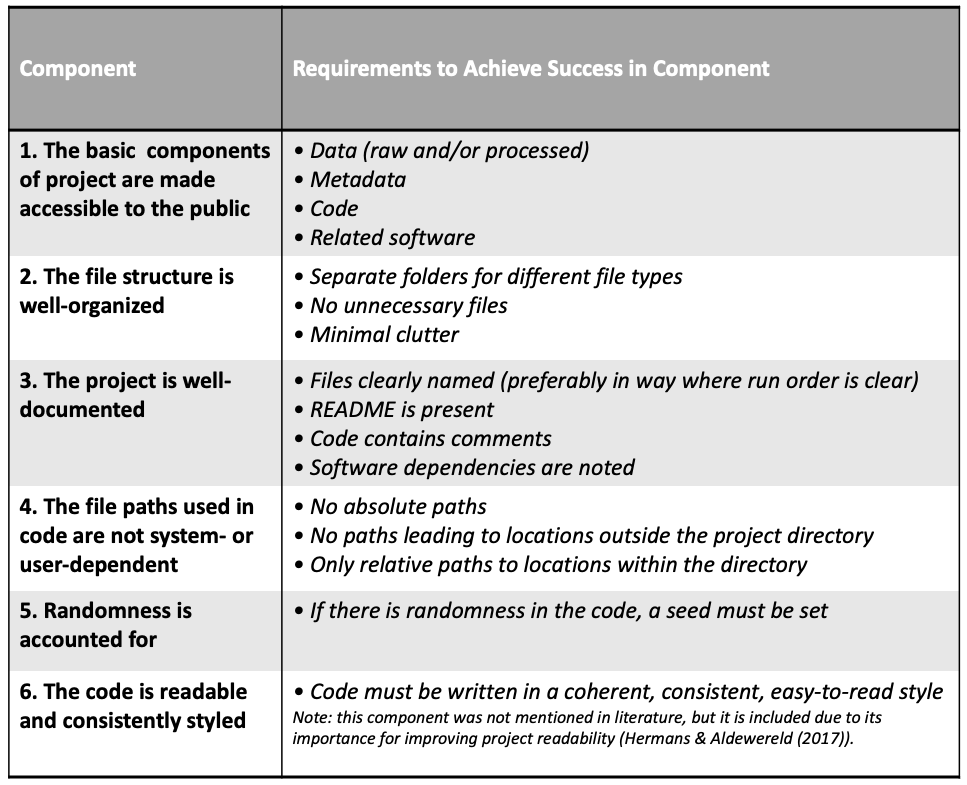
\includegraphics[width=1\linewidth]{figure/6-components} \caption{The 6 Major Components of Reproducibility --- Accessibility, organization, documentation, good file paths, controlled randomness, style/readability.}\label{fig:unnamed-chunk-4}
\end{figure}
\hypertarget{current-attempts-to-address-reproducibility-in-scientific-publishing}{%
\section{Current Attempts to Address Reproducibility in Scientific Publishing}\label{current-attempts-to-address-reproducibility-in-scientific-publishing}}

In an attempt to increase reproducibility, leaders from academic journals around the world have taken steps to create new standards and requirements for submitted articles. These standards attempt to address the components of reproducibility listed previously, requesting that authors provide certain materials necessary for reproducing their work when they submit an article. However, these standards are highly inconsistent, varying significantly both across and within disciplines, and many only cover one or two of the six primary components, if any at all.

To illustrate this point, we will consider several case studies from journals publishing research on a variety of scientific fields.

\hypertarget{case-studies-across-the-sciences}{%
\subsection{Case Studies Across The Sciences}\label{case-studies-across-the-sciences}}

The journal whose requirements appear to align most closely with those components defined previously in Section 3 is the \emph{American Journal of Political Science} (AJPS). In 2012, the AJPS became the first political science journal to require authors to make their data openly accessible online, and the publication has instituted stricter requirements since. AJPS now requires that authors submit the following alongside their papers (AJPS Staff (2016)).
\begin{itemize}
\tightlist
\item
  The dataset analyzed in the paper and information about its source. If the dataset has been processed, instructions for manipulating the raw data to achieve the final data must also be shared.
\item
  Detailed, clear code necessary for reproducing all of the tables and figures in the paper. Note that this requirement goes beyond most of what is recommended in reproducibility literature, which simply recommends code to produce the analysis results---and not necessarily all outputs.
\item
  Documentation, including a README and codebook.
\item
  Information about the software used to conduct the analysis, including the specific versions and packages used.
\end{itemize}
These standards are quite thorough and contain mandates for the inclusion of the vast majority of components necessary for complete reproducibility. Most journals, however, do not come close to meeting such high standards in their reproducibility statements.

For example, in the biomedical sciences, a group of editors representing over 30 major journals met in 2014 to address reproducibility in their field, coming to a consensus on a set of principles they wanted to uphold (National Institutes of Health (2014)). Listed below are those relating specifically to the use of data and statistical methods:
\begin{enumerate}
\def\labelenumi{\arabic{enumi})}
\item
  Journals in the biomedical sciences should have a mechanism to check the statistical accuracy of submissions.
\item
  Journals should have no (or generous) limit on methods section length.
\item
  Journals should use a checklist to ensure the reporting of key information, including:
\end{enumerate}
\begin{itemize}
\tightlist
\item
  The article meets nomenclature/reporting standards of the biomedical field.
\item
  Investigators report how often each experiment was performed and whether results were substantiated by repetition under a range of conditions.
\item
  Statistics must be fully reported in the paper (including test used, value of \texttt{N}, definition of center, dispersion and precision measures).
\item
  Authors must state whether samples were randomized and how.
\item
  Authors must state whether the experiment was blinded.
\item
  Authors must clearly state the criteria used for exclusion of any data or subjects and must include all results, even those that do not support the main findings.
\end{itemize}
\begin{enumerate}
\def\labelenumi{\arabic{enumi})}
\setcounter{enumi}{3}
\item
  All datasets used in analysis must be made available on request and should be hosted on public repositories when possible. If not possible, data values should be presented in the paper or supplementary information.
\item
  Software sharing should be encouraged. At the minimum, authors should provide a statement describing if software is available and how to obtain it.
\end{enumerate}
Even though these principles seem well-developed on the surface, they fail to meet even the basic requirements defined by Goodman, Fanelli, \& Ioannidis (2016) previously. Several of the principles are purely recommendations; there is no requirement that code be shared, nor metadata. Additionally, software requirements are quite loose. No information about dependencies or software version needs to be included. Beyond that, there is not even a requirement that analysis be completed in a scriptable programming language---allowing for the potential that some submitted work may be entirely non-reproducible due to its format.

We see a similar issue even in journals designed specifically for the purpose of improving scientific reproducibility. \emph{Experimental Results}, a publication created by Cambridge University Press to address some of the reproducibility and open access issues in academia, also falls short of meeting high standards. The journal, which showcases articles from a variety of scientific decisions disciplines, states in their transparency and openness policy:
\begin{quote}
Whenever possible authors should make evidence and resources that underpin published findings, such as data, code, and other materials, available to readers without undue barriers to access.
\end{quote}
The inclusion of code and data are only recommended and no definition of what ``other materials'' may mean is provided. No components of reproducibility extending beyond those required at a minimum are even considered (Cambridge University Press (2020)).

The \emph{American Economic Review}, the first of the top economics journals to require the inclusion of data alongside publications, has stronger guidelines than several of those mentioned previously, though not as strong as the \emph{American Journal of Political Science}. Their Data and Code Availability Policy states the following (AEA Staff (2020)):
\begin{quote}
It is the policy of the American Economic Association to publish papers only if the data and code used in the analysis are clearly and precisely documented, and access to the data and code is clearly and precisely documented and is non-exclusive to the authors.
\end{quote}
These requirements are quite strict, prohibiting exceptions for papers using data or code not available to the public in the way that many other journals claiming to promote reproducibility do.

\hypertarget{case-studies-in-the-statistical-and-data-sciences}{%
\subsection{Case Studies in the Statistical and Data Sciences}\label{case-studies-in-the-statistical-and-data-sciences}}

When considering reproducibility policy, the field of Statistical and Data Sciences performs relatively well. The majority of highly ranked journals in the field contain statements on reproducibility. Some of these are quite robust, surpassing the requirements of many of the other journals discussed previously, while others are lacking.

In this section, we'll consider in detail the reproducibility policies of some of these top journals, selected by a compound measure of influence, impact, and prestige---which summarizes the average number of weighted citations received in a given year compared with the number of documents published in that journal over the previous three years---calculated for the year 2020 (see \url{https://www.scimagojr.com/journalrank.php?category=2613}).

The \emph{Journal of the American Statistical Association} stands out as having relatively robust requirements. The publication's guidelines require that data be made publicly available at the time of publication except for reasons of security or confidentiality. It is strongly recommended that code be deposited in open repositories. If data is used in a processed form, the provided code should include the necessary cleaning/preparation steps. Data must be in an easily understood form and a data dictionary should be included. Code should also be in a form that can be used and understood by others, including consistent and readable syntax and comments. Workflows involving more than one script should also contain a master script, Makefile, or other mechanism that makes it clear what each component does, in what order to run them, and what the inputs and outputs to each area (JASA Staff (2020)).

The \emph{Journal of Statistical Software} also has strong guidelines, though less thorough. Authors must provide \emph{commented} source code for their software; all figures, tables, and output must be exactly reproducible on at least one platform; random number generation must be controlled; and replication materials (typically in the form of a script) must be provided (JSS Staff (2020)).

The expectations of the \emph{Journal of Computational and Graphical Statistics} are notably weaker, requiring only that authors ``submit code and datasets as online supplements to the manuscript,'' with exceptions for security or confidentiality, but providing no further detail (JCGS Staff (2020)). The \emph{R Journal} has the same requirements, but with no exceptions on the data provision policy, stating that authors should ``not use such datasets as examples'' (R Journal Editors (2020)).

Perhaps the least strict reproducibility policies come from \emph{The American Statistician} and the \emph{Annals of Statistics}. The former appears to have no requirements, stating only that it ``strongly encourages authors to submit datasets, code, other programs, and/or appendices that are directly relevant to their submitted articles,'' while the latter appears to have no statement on reproducibility at all (American Statistician Staff (2020)).
\begin{figure}

{\centering 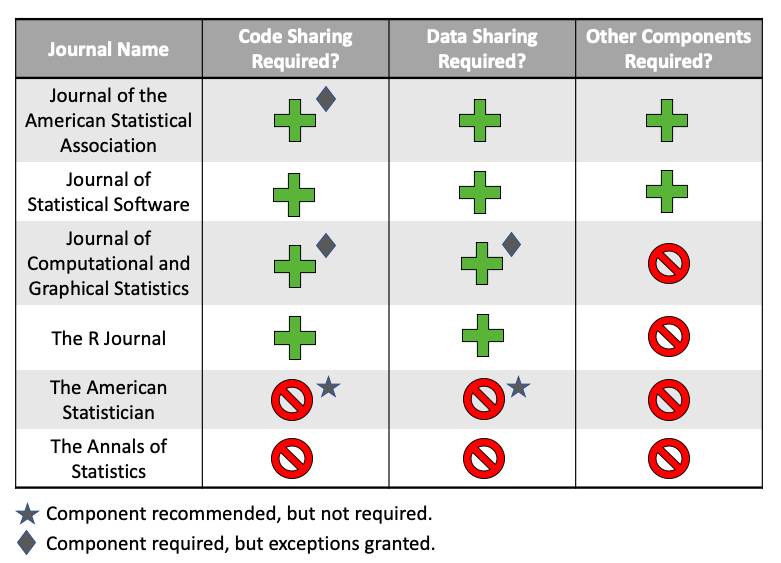
\includegraphics[width=1\linewidth]{figure/stats-journals} 

}

\caption{Reprodubility Policies of Top Statistical and Data Sciences Journals --- JASA and JSS have the strongest reproducibility requirements, while The American Statistician and The Annals of Statistics have next to none.}\label{fig:unnamed-chunk-5}
\end{figure}
\hypertarget{the-bigger-picture}{%
\subsection{The Bigger Picture}\label{the-bigger-picture}}

The journals mentioned here are just some of the many academic publishers with reproducibility policies. While they provide a sense of the specific wording and requirements of some policies, they do not necessarily serve as a representative sample of all academic publishing. It is important to also consider the bigger picture, exploring the state of reproducibility policy in academic publishing as a whole.

Given the scale of the academic publishing network and the sheer number of journals around the world, this is not necessarily an easy task.

In order to simplify this process, academics at the Center for Open Science (COS) attempted to create a metric, called the TOP Factor. The TOP Factor reports the steps that a journal is taking to implement open science practices. It has been calculated for a wide variety of journals, though the COS is still far from scoring all of the publications that are currently available.
\begin{center}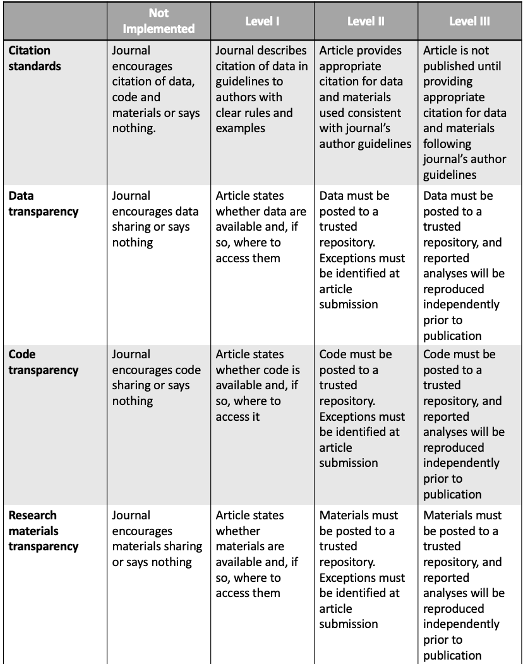
\includegraphics[width=1\linewidth]{figure/top-1} \end{center}
\begin{figure}

{\centering 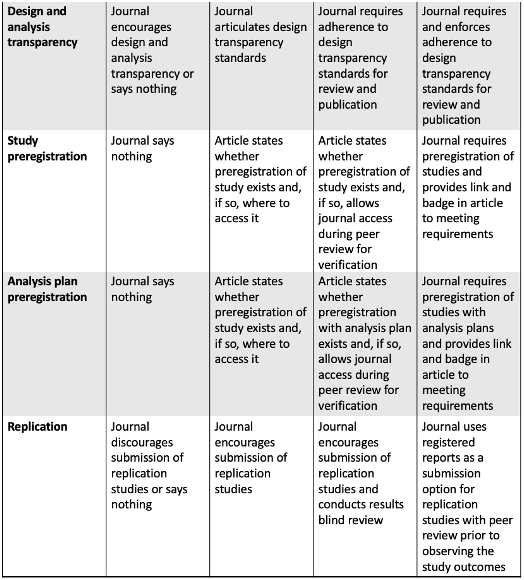
\includegraphics[width=1\linewidth]{figure/top-2} 

}

\caption{The TOP Factor Rubric --- The TOP Factor method uses an eight category rubric to measure reproducibility in the sciences.}\label{fig:top-factor2}
\end{figure}
The TOP Factor is calculated as follows. Publications are scored on a variety of categories associated with open science and reproducibility. For each category, they receive a score between 0 (poor) and 3 (excellent) based on the degree to which they emphasize each category in their submission/publication policies. A journal's final score, which can range from 0 to 30, is the sum of the individual scores in each of the categories.

When looking at the overall distribution of TOP Factor scores, we see a relatively grim picture: Around 50\% of journals score as low as 0-5 overall, while only just over 5\% score more than 15, just half of the maximum possible score. Over 40 journals failed to score a single point (Woolston (2020)).

\hypertarget{assessing-the-success-of-academic-reproducibility-policies}{%
\subsection{Assessing the Success of Academic Reproducibility Policies}\label{assessing-the-success-of-academic-reproducibility-policies}}

We have seen that, although not necessarily the standard, some journals from across the sciences have enacted reproducibility policies. The simple implementation of a policy, however, does not ensure that its goals will be achieved. Reproducibility can only be addressed when both authors \emph{and} journal reviewers actively implement publishing standards in practice. Without participation and dedication from all involved, reproducibility guidelines serve more as a theoretical goal than a practical achievement.

It is important to ask, then, whether academic reproducibility standards \emph{actually} result in a greater number of reproducible publications.

Let us consider the case of the journal \emph{Science}. \emph{Science} instituted a reproducibility policy in 2011 and has maintained it ever since. In its original form, their policy stated the following:
\begin{quote}
All data necessary to understand, assess, and extend the conclusions of the manuscript must be available to any reader of Science. All computer codes involved in the creation or analysis of data must also be available to any reader of Science. After publication, all reasonable requests for data and materials must be fulfilled. Any restrictions on the availability of data, codes, or materials\ldots must be disclosed to the editors upon submission\ldots{}
\end{quote}
This policy is similar to many of the others considered previously, requiring the publishing of code and data with exceptions permitted when necessary.

Stodden, Seiler, \& Ma (2018) tested the efficacy of this policy in practice, emailing corresponding authors of 204 articles published in the year after \emph{Science} first implemented its policy to request the data and code associated with their articles. The researchers only received (at least some of) the requested material from 36\% of authors. This low rates were due to several factors:
\begin{itemize}
\tightlist
\item
  26\% of authors did not respond to email contact.
\item
  11\% of authors were unwilling to provide the data or code without further information regarding the researchers' intentions.
\item
  11\% asked the researchers to contact someone else and that person did not respond.
\item
  7\% refused to share data and/or code.
\item
  3\% directed the researchers back to their paper's supplemental information section.
\item
  3\% of authors made a promise to follow up and then did not follow through.
\item
  3\% of emails bounced.
\item
  2\% gave reasons why they could not share for ethical reasons, size limitations, or some other reason.
\end{itemize}
Of the 56 papers they deemed likely reproducible, the authors randomly selected 22 and were able to replicate the results for all but 1, which failed due to its reliance on software that was no longer available.

Hardwicke et al. (2018) compared the reproducibility of published work both before and after the journal \emph{Cognition} instituted an open data policy, that required authors to make relevant research data publicly available prior to publication of an article.

The researchers found a considerable increase in the proportion of data available statements (in contrast to `data not available' statements, which could be present due to privacy or security concerns) since the implementation of the policy. Pre-open data policy, only 25\% of articles had data available, while that number was a much higher 78\% after the policy was put in place.

While the institution of an open data policy appears to have been associated with a significant increase in the percentage of studies with data available, further research indicates that the policy was perhaps not as effective as intended. Many of the datasets were usable in theory, but not in practice. Only 62\% of the articles with data available statements had truly reusable datasets---in this case, meaning that the data were accessible, complete, and understandable. Although this is an increase from the pre-policy period, which saw 49\% of articles with data availability statements as reusable in practice, it is still far from ideal.

In this small sample of cases, we see that purely having a reproducibility statement does not necessarily mean that all, or even a majority, of published work will truly be reproducible.

\hypertarget{limitations-on-achieving-reproducibility-in-scientific-publishing}{%
\section{Limitations on Achieving Reproducibility in Scientific Publishing}\label{limitations-on-achieving-reproducibility-in-scientific-publishing}}

There are several reasons for this apparent divide between journal reproducibility standards and the proportion of submitted articles that are truly reproducible. Some of these are challenges faced by the article authors, while others are faced by the journal editors.

\hypertarget{challenges-for-authors}{%
\subsection{Challenges for Authors}\label{challenges-for-authors}}

Stodden, Seiler, \& Ma (2018) conducted a survey asking over 7,700 researchers about one of the key characteristics of reproducibility---open data---and gathered information about the reasons why authors found difficulties in making their data available to the public

The main challenges listed by respondents were as follows:
\begin{itemize}
\tightlist
\item
  46\% identified ``Organizing data in a presentable and useful way'' to be difficult.
\item
  37\% had been ``Unsure about copyright and licensing.''
\item
  33\% had problems with ``Not knowing which repository to use.''
\item
  26\% cited a ``Lack of time to deposit data.''
\item
  19\% found the ``Costs of sharing data'' to be high.
\end{itemize}
The relative frequency of these issues varied across several characteristics, including author seniority, subject area, and geographical location, though authors in all categories faced some issues.

Beyond technical challenges, other reasons may lead authors to not place their focus on reproducibility. For example, some researchers might fear damage to their reputation if a reproduction attempt fails after they have provided the necessary materials (Lupia \& Elman (2014)).

Given the importance of achieving reproducibility, it follows that researchers will not make the necessary effort to do so if journal guidelines provide a way out. Policies that \emph{recommend} the inclusion of data or that allow exceptions to open data for certain reasons are likely to be associated with a lower proportion of reproducible articles than those that make open data mandatory.

\hypertarget{challenges-for-journals}{%
\subsection{Challenges for Journals}\label{challenges-for-journals}}

In addition to the challenges faced on the part of the authors, journal reviewers face their own difficulties in ensuring reproducibility.

In order to make sure that all submitted articles comply with reproducibility guidelines, reviewers must go through them one by one and reproduce all of the results by hand using the provided materials.

This is a very time and labor intensive process, as we will see in the example of the \emph{American Journal for Political Science} (AJPS), whose reproducibility policy was discussed previously in Chapter 1.4.1.

Jacoby, Lafferty-Hess, \& Christian (2017) describe the AJPS process in detail:
\begin{quote}
Acceptance of a manuscript for publication in the AJPS is contingent on successful replication of any empirical analyses reported in the article.
\end{quote}
After an article is submitted, staff from a third party vendor hired by AJPS go through the provided materials to ensure that they can be preserved, understood, and used by others. They then run all of the analyses in the article using the code, instructions, and data provided by the authors and compare their results to the submitted articles. Authors are then given an opportunity to resolve any issues that come up. This process is repeated until reproducibility is ensured.

Although providing a significant benefit to the scientific community, this thorough process is associated with high costs.

The verification process slows down the journal review process significantly, adding a median 53 days to the publication workflow, as many submitted articles require one or more rounds of re-submission (the average number of re-submissions is 1.7). It is also quite labor intensive, taking an average of 8 person-hours per manuscript to reproduce the analyses and prepare the materials for public release and adding significant monetary cost to AJPS.

Journals are often reluctant to take on such an intensive task due to the drastically increased burden it places on reviewers and on the publication's financial resources. This is particularly true given that the number of submitted articles per year has been increasing over time (Leopold (2015)). Every additional submission increases the burden of achieving reproducibility, and with a large enough volume, the challenge can quickly become seemingly impossible to manage reasonably.

Reviewers themselves are also not inclined to support an increased focus on reproducibility. AJPS is an exception, but Journal review is often not a paid position. In many cases, reviewers are obligated to participate as part of their expected contribution to academia. They receive no compensation for their efforts and every additional hour of labor is an unwanted burden. Any changes that add complication to the review process are not desirable; although reproducibility may be important, reviewers are not likely to support a focus on it unless the process is streamlined.

As a result, journals often encourage reviewers to consider authors' compliance with data sharing policies, but do not formally require that they ensure it as a criterion for acceptance (Hrynaszkiewicz (2020)).

\hypertarget{attempts-to-address-these-limitations}{%
\section{Attempts to Address These Limitations}\label{attempts-to-address-these-limitations}}

The previous discussion makes clear that, although reproducibility is critically important to scientific progress and academic journals are taking steps to encourage it, the scientific community is far from achieving the desired level of widespread reproducibility. In large part, this appears due to the challenge and complexity of actually achieving reproducibility. Those attempting to improve the reproducibility of work can face challenges over legality of sharing data, large commitments of time or money, difficulties in finding a good repository and organizing all of the many components of their work in an understandable way, among other things.

Additionally, science faces the additional challenge that many publishers do not emphasize reproducibility at all, providing many opportunities for all authors except those personally dedicated to producing reproducible work to leave reproducibility by the wayside. Many journals have no reproducibility requirements, and those that do often do not take the necessary steps to ensure that they are actually met.

These issues, however, are not impossible to overcome. Proponents of reproducibility have taken action to help address them, both through education on reproducibility and through software that helps simplify the process of achieving it.

\hypertarget{through-education}{%
\subsection{Through Education}\label{through-education}}

One way to address the reproducibility crisis is to educate data analysts on the topic so that they are aware of both the concept of reproducibility and how to achieve it in their own work. A natural place to focus this education is early on in the data science training pipeline as part of introductory or early-intermediate courses in undergraduate and graduate data science programs (Horton, Baumer, \& Wickham (2015)). This sort of educational integration has a variety of benefits:
\begin{itemize}
\item
  Bringing reproducibility into the discussion early on gives students the tools to add knowledge to their field in the best way possible before they actually conduct any substantive analysis on their own (Janz (2016)). This produces many long run benefits, helping to lessen the burden on promoting reproducibility placed on journals and increasing the number (and percentage) of researchers doing and promoting reproducible work.
\item
  If covered in detail as part of the data science curriculum, reproducibility will eventually seem natural to students. If learned independently, without effective tools, it can be challenging and even disheartening to try to understand and succeed at achieving reproducibility. Practicing in the classroom gives students the ability to fail without damaging their reputation, giving a great opportunity to truly learn and understand the concepts so that they feel capable of handling them when they begin their own research.
\item
  The application of grading to the topic provides an incentive for students to pay attention, learn, and absorb the information. This same incentive does not exist when researchers attempt to learn about reproducibility independently. In that situation, internal motivation, which may be weak in some individuals, is the only factor present to help promote success.
\end{itemize}
Several educators, primarily at the graduate level, have realized the opportunity and have taken steps to introduce reproducibility into their courses.
According to Janz (2016), the primary way of achieving this integration is through the assignment of ``replication studies'' in standard methods choices. In these assignments, students are given a published study and its supporting materials and asked to reproduce the results. One course of this kind is Government 2001, taught by Gary King at Harvard University. In King's course, students team up in small groups to reproduce a previous study. To help ensure that their workflow is reproducible, students are required to hand over their data and code to another student team who then tries to reproduce their work once again.

In Thomas M. Carsey's intermediate statistics course at the University of North Carolina at Chapel Hill, students must reproduce the findings of a study by re-collecting the data from the original sources, then must extend the study by building on the analysis.

Christopher Fariss of Penn State University asks his students to replicate a research paper published in the last five years, noting that students must describe the article and the ease in which the results replicate.

The University of California at Berkeley has a similar course to Gary King's Harvard course, where students each take a different piece of an existing study to work on reproducing and have to ensure that their piece fits with the piece of the next student (Hillenbrand (2014)).

At the undergraduate level, rather than assign replication studies the way many graduate schools tend to do, Smith College and Duke University have both integrated reproducibility into their introductory courses through the requirement that assignments be completed in the \texttt{RMarkdown} code + narration format (Baumer, Cetinkaya-Rundel, Bray, Loi, \& Horton (2014)).

Another way to provide education on reproducibility is through the creation of workshops that focus solely on the topic, rather than through integration as just one part of a class (Janz (2016)).

For example, the University of Cambridge conducts a Replication Workshop, where graduate students are asked replicate a paper in their field over eight weekly sessions. When students encounter challenges, such as authors not responding to queries for data or steps of the analysis being poorly defined and explained, they gain a first hand understanding of the consequences of poor transparency.

Workshops such as these are typically optional and not included as part of the primary curriculum, however, so while they may cover the topic of reproducibility in more detail than traditional courses, they often reach fewer students.

In spite of all of the advantages that these educational tools provide, ``reproducibility training and assessment in data science education is largely neglected, especially among undergraduates and Master's students in professional schools\ldots, probably because the students are usually considered to be non-research oriented'' (Yu \& Hu (2019)). While some examples of reproducibility education exist, they are certainly not commonplace. However, given the increased discussion and emphasis on reproducibility in academia over the past several years, it is likely that this will change, particularly if methods are provided to educators to make the integration of reproducibility into their courses simple and relatively unburdensome.

\hypertarget{through-software}{%
\subsection{Through Software}\label{through-software}}

Several researchers and members of the Statistical and Data Sciences community have taken action to develop software focused on reproducibility which removes some of the load on data analysts by automating reproducibility processes and checking whether certain components are achieved.

Much of this software has been written for users of the coding and data analysis language \texttt{R}. \texttt{R} is very popular in the data science community due to its open-source nature, accessibility, extensive developer and user base, and statistical analysis-specific features.

Some of the existing software solutions are listed below:

\texttt{rrtools} (Marwick (2019)) addresses many of the issues discussed in Marwick, Boettiger, \& Mullen (2018) by creating a basic reproducible structure based on the \texttt{R} package format for a data analysis project. In addition, it allows for isolation of the computer environment using \texttt{Docker}, provides a method to capture information about the versions of packages used in a project, contains tools for generating a README file, and provides an option for users to write tests to check that their functions operate as intended.

The \texttt{orderly} (FitzJohn et al. (2020)) package also focuses on file structure, requiring the user to declare a desired project structure (typically a step-by-step structure, where outputs from one step are inputs into the next) at the beginning and then creating the files necessary to achieve that structure. Its principal aim is to automate many of the basic steps involved in writing analyses, making it simple to:
\begin{enumerate}
\def\labelenumi{\arabic{enumi})}
\tightlist
\item
  Track all inputs into an analysis;
\item
  Store multiple versions of an analysis where it is repeated;
\item
  Track outputs of an analysis; and
\item
  Create analyses that depend on the outputs of previous analyses.
\end{enumerate}
When projects have a variety of components, \texttt{orderly} makes it easy to see inputs and outputs change with each re-run.

\texttt{workflowr}'s (Blischak, Carbonetto, \& Stephens (2019)) functionality is based around version control and making code easily available online. It works to generate a website containing time-stamped, versioned, and documented results. In addition, it manages the session and package information of each analysis and controls random number generation.

\texttt{checkers} (Ross, DeCicco, \& Randhawa (2018)) allows you to create custom checks that examine different aspects of reproducibility. It also contains some pre-built checks, such as seeing if users reference packages that are less preferred to other similar ones and ensuring that the project is under version control.

\texttt{renv} (Ushey \& RStudio (2020)) (formerly \texttt{packrat}) helps to make projects more isolated, portable, and reproducible. It gives every project its own private package library, makes it easy to install the packages the project depends on if it is moved to another computer.

\texttt{drake} (R OpenSci (2020)) analyzes workflows, skips steps where results are up to date, utilizes optimized computing to complete the rest of the steps, and provides evidence that results match the underlying code and data.

Lastly, the \texttt{reproducible} (McIntire \& Chubaty (2020)) package focuses on the concept of caching: saving information so that projects can be run faster each time they are re-completed from the start.
\begin{figure}

{\centering 
\includegraphics[width=0.5\linewidth]{figure/packages} 

}

\caption{Popular Reproducibility Packages in R --- Drake, packrat (now renv) and workflowr are some of the more well-known reproducibility-focused R packages.}\label{fig:unnamed-chunk-6}
\end{figure}
There have also been several \texttt{Continuous\ integration} tools developed outside of R which can be used by those coding in almost any language. These provide more general approaches to automated checking, which can enhance reproducibility with minimal code.

For example, \texttt{wercker}---a command line tool that leverages Docker---enables users to test whether their projects will successfully compile when run on a variety of operating systems without access to the user's local hard drive (Oracle Corporation (2019)).

\texttt{GitHub\ Actions} is integrated into GitHub and can be configured to do similar checks on projects hosted in repositories.

\texttt{Travis\ CI} and \texttt{Circle\ CI} are popular continuous integration tools that can also be used to check \texttt{R} code.
\begin{figure}

{\centering 
\includegraphics[width=0.8\linewidth]{figure/ci-tools} 

}

\caption{Popular Continuous Integration Tools --- Many of these tools are integrated into other tools, like GitHub, making them easily accessible.}\label{fig:unnamed-chunk-7}
\end{figure}
\hypertarget{understanding-the-gaps-in-existing-reproducibility-solutions}{%
\section{Understanding The Gaps In Existing Reproducibility Solutions}\label{understanding-the-gaps-in-existing-reproducibility-solutions}}

Although the current state of reproducibility in academia is quite poor, it is not an impossible challenge to overcome. The relative simplicity of addressing reproducibility, particularly when compared with replicability, makes it an ideal candidate for solution-building. Although significant progress on addressing reproducibility on a widespread scale is a long-term challenge, impactful forward progress---if on a smaller scale---can be achieved in the short-term.

As we have seen, software developers, data scientists, and educators around the world have realized this potential, taking steps to help address the current crisis of reproducibility. Journals have put in place guidelines for authors, statisticians have developed \texttt{R} packages that help structure projects in a reproducible format, and educators have begun integrate reproducibility exercises into their courses.

We have already explored the issues with journal policies, both for authors and reviewers, in-depth. Educational and software-based strategies attempt to address these policy issues by spreading ideas of reproducibility to more people and simplifying the process of achieving it, therefore resulting (in theory) in an improvement in the reproducibility of published scientific articles.

However, the reality is not quite so rosy. Many current educational and software-based solutions face their own challenges that limit them from achieving the desired outcome. In this section, we will consider these issues.

\hypertarget{in-education}{%
\subsection{In Education}\label{in-education}}

The two primary concerns about the integration of reproducibility in data science curricula revolve around time and difficulty.

As noted previously, the primary mode of teaching reproducibility is through the assignment of replication studies where students must take an existing study and go through the process of reproducing it themselves, including contacting the author for all necessary materials, rerunning code and analysis, and problem-solving when issues almost certainly come up.

In addition to the time required for the professor to collect all of the studies that students will be working on, the inclusion of such an assignment places a significant burden on educators by taking up time where they could be teaching other important material. Replication studies, if done correctly, can take weeks for students to successfully complete. The choice to give such assignments is therefore associated with a significant opportunity cost which many professors are unwilling to take.

Additionally, both replication studies assigned in class and replication workshops outside of normal coursework require a working knowledge of how to successfully complete and understand research. This makes them inaccessible to individuals who are still in their undergraduate career and may not yet have had an opportunity to conduct research or those who are studying in non-research-focused technical programs.

In order to reach the widest variety of students possible, it is necessary to develop a new method of teaching reproducibility that is neither time consuming nor dependent on a prior understanding of the research process.

\hypertarget{in-software}{%
\subsection{In Software}\label{in-software}}

Previously, we considered several different types of software solutions: packages designed for users of \texttt{R} and continuous integration programs that can be used alongside a variety of coding languages. Although these solutions have their advantages, they also have significant drawbacks in terms of their ability to address reproducibility on a widespread scale.

Many of the packages designed for \texttt{R} are narrow in scope, with each effectively addressing a small component of reproducibility: file structure, modularization of code, version control, etc. They often succeed in their area of focus, but at the cost of accessibility to a wider audience. Their functions are often quite complex to use, and many steps must be completed to achieve the required reproducibility goal. This cumbersome nature means that most reproducibility packages currently available are not easily accessible to users with minimal \texttt{R} experience, nor particularly useful to those looking for quick and easy reproducibility checks. Their significant learning curve can also drive away potential users who may be interested in reproducibility but not willing to dedicate an extensive amount of time to understanding the intricacies of software operation.

Due to their generalized design, Continuous Integration tools do not face the same issues with narrowness or complexity that \texttt{R} packages struggle with. However, this generalizability provides its own additional challenge. Since Continuous Integration tools are designed to be accessible to a wide variety of users with different coding preferences, they are not particularly user-friendly and lack the ability to address features specific to certain programming languages.

\hypertarget{what-we-need-moving-forward}{%
\subsection{What We Need Moving Forward}\label{what-we-need-moving-forward}}

While a variety of attempts to address reproducibility have been made, they all face their own set of challenges. Most focus on only one area of reproducibility, are too time consuming and burdensome to attempt, or require an extensive amount of background knowledge.

In order to truly improve scientific reproducibility, a better solution is needed. The optimal solution should combine the positive aspects of the previously discussed educational and software methods, while remaining simple and easy to use. It should also have a variety of potential applications---journal reviewers should benefit from it, as should authors, as should educators and students and even those outside of academia.

The full list of necessary features for an effective reproducibility tool are provided below:
\begin{enumerate}
\def\labelenumi{\arabic{enumi})}
\tightlist
\item
  Be simple, with a small library of functions/tools that are straightforward to use.
\item
  Be accessible to a variety of users, with a relatively small learning curve.
\item
  Be able to address a wide variety of aspects of reproducibility, rather than just one or two key issues.
\item
  Have features specific to a particular coding language that can address that language's unique challenges.
\item
  Be customizable, allowing users to choose for themselves which aspects of reproducibility they want to focus on.
\item
  Be educational, teaching those that use it about why their projects are not reproducible and how to correct that in the future.
\item
  Be applicable to a wide variety of domains.
\end{enumerate}
While this seems like a lot to ask, such a task is not impossible. In the next chapter, we will consider one potential solution: \texttt{fertile}, an R package focused on reproducibility that I developed.

\hypertarget{my-solution}{%
\chapter{\texorpdfstring{\texttt{fertile}: My Contribution To Addressing Reproducibility}{fertile: My Contribution To Addressing Reproducibility}}\label{my-solution}}

\hypertarget{fertile-an-r-package-creating-optimal-conditions-for-reproducibility}{%
\section{\texorpdfstring{\texttt{fertile}, An R Package Creating Optimal Conditions For Reproducibility}{fertile, An R Package Creating Optimal Conditions For Reproducibility}}\label{fertile-an-r-package-creating-optimal-conditions-for-reproducibility}}

\texttt{fertile} is an \texttt{R} package that attempts to combine the 7 key features of an effective reproducibility tool, discussed at the end of Chapter 1, into a singular piece of software that can be easily downloaded, installed, and operated by \texttt{R} users.
\begin{figure}

{\centering 
\includegraphics[width=0.3\linewidth]{figure/fertile-hex} 

}

\caption{fertile's Package Logo}\label{fig:unnamed-chunk-8}
\end{figure}
\texttt{fertile} attempts to address the gaps in existing reproducibility solutions by combining software and education in one product. The package provides a set of simple, easy-to-learn tools that, rather than focus intensely on a specific area like other software programs, provide some information about all six major components of reproducibility. It is also designed to be flexible, offering benefits to users at any stage in the data analysis workflow and providing users with the option to select which aspects of reproducibility they want to focus on.

\texttt{fertile} also contains several \texttt{R}-specific features, which address certain aspects of reproducibility that can be missed by external project development tools. It is designed primarily to be used on data analyses organized as \texttt{R} Projects (i.e.~directories containing an \texttt{.Rproj} file) and contains several associated features to ensure that the project structure meets the standards discussed in the \texttt{R} community.

In addition, \texttt{fertile} is designed to be educational, teaching its users about the components of reproducibility and how to achieve them in their work. The package provides users with detailed reports on the aspects of reproducibility where their projects fell short, identifying the root causes and, in many cases, providing a recommended solution.

\texttt{fertile} is structured in such a way as to be understandable and operable to individuals of any skill level, from students in their first undergraduate data science course to experienced PhD statisticians. The majority of its tools can be accessed in only a handful of functions with minimal required arguments. This simplicity makes the process of achieving and learning about reproducibility accessible to a wide audience in a way that complex software programs or graduate courses requiring an advanced knowledge of research methods do not.

Reproducibility is significantly easier to achieve when all of the tools necessary to do so are located in one place. \texttt{fertile} provides this optimal all-inclusive structure, addressing all 6 major components of reproducibility. We will consider \texttt{fertile}'s treatment of each of these components in turn, exploring its behavior using the sample R project shown below, titled \texttt{project\_miceps}:
\begin{figure}
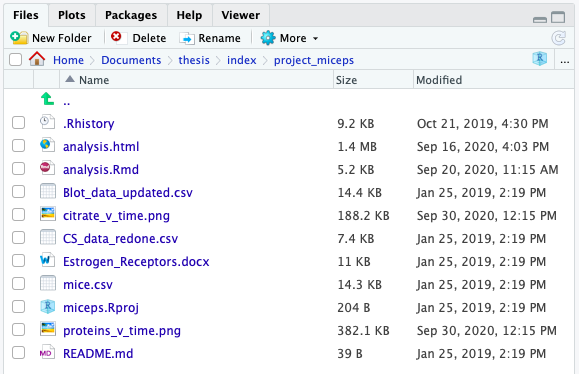
\includegraphics[width=1\linewidth]{figure/sample-project} \caption{A Sample R Project}\label{fig:unnamed-chunk-9}
\end{figure}
\texttt{project\_miceps} contains data and analysis from a study concerning the differences in bicep muscle growth between male and female mice, conducted under Smith College professor Stylianos Scordilis.

The folder contains a variety of different file types:
\begin{itemize}
\tightlist
\item
  1 \texttt{.Rmd} file containing the analysis code. This involves data manipulation, visualization, and random number generation
\item
  1 \texttt{.html} containing the knitted output of the analysis code
\item
  3 \texttt{.csv} files containing the experimental data
\item
  2 \texttt{.png} image files containing plot outputs from the analysis
\item
  1 \texttt{README} file containing information about the project
\item
  A \texttt{.docx} file containing text about estrogen receptors in mice
\item
  \texttt{.Rproj} and \texttt{.Rhistory} files, containing data used by \texttt{R} to track work and maintain the project structure
\end{itemize}
In the following sections, we will consider the functionality of \texttt{fertile} as demonstrated primarily through the results of a reproducibility analysis conducted on \texttt{project\_miceps}. All of the code for \texttt{fertile} that will be discussed in this chapter can be found at \url{https://github.com/baumer-lab/fertile}, while the local branch tracking my changes can be found at \url{https://github.com/ambertin/fertile}.

\hypertarget{component-1-accessible-project-files}{%
\subsection{Component 1: Accessible Project Files}\label{component-1-accessible-project-files}}

The inclusion of key files---such as analysis scripts, data, and documentation information---helps ensure reproducibility by providing the audience with access to everything relevant and necessary to the process of re-running a project.
\begin{Shaded}
\begin{Highlighting}[]
\FunctionTok{library}\NormalTok{(fertile)}
\end{Highlighting}
\end{Shaded}
\texttt{fertile} takes several steps to help users ensure that all of files necessary to run an analysis are provided in the project folder.

\hypertarget{file-overview}{%
\subsubsection{File Overview}\label{file-overview}}

One way to gain an overview of the existing files (including data, code, and metadata) is with the \texttt{proj\_analyze\_files()} function. It lists all of the files in the project, along with their size, type, and relative path within the directory. This can help users quickly produce an overview of how many code, data, and auxiliary (image or text) files they have.

When this is run on \texttt{project\_miceps}, we see the same files as described before--their names, file sizes, extensions, and a MIME type, which summarizes the file format using a two-part identifier.
\begin{Shaded}
\begin{Highlighting}[]
\FunctionTok{proj\_analyze\_files}\NormalTok{(}\StringTok{"project\_miceps"}\NormalTok{)}
\end{Highlighting}
\end{Shaded}
\footnotesize
\begin{verbatim}
# A tibble: 11 x 5
   file                     size ext   mime                       path_rel      
   <fs::path>           <fs::by> <chr> <chr>                      <fs::path>    
 1 project_miceps/Blot~   14.43K csv   text/csv                   Blot_data_upd~
 2 project_miceps/CS_d~    7.39K csv   text/csv                   CS_data_redon~
 3 project_miceps/Estr~   10.97K docx  application/vnd.openxmlfo~ Estrogen_Rece~
 4 project_miceps/READ~       39 md    text/markdown              README.md     
 5 project_miceps/anal~    5.21K Rmd   text/x-markdown            analysis.Rmd  
 6 project_miceps/anal~    1.41M html  text/html                  analysis.html 
 7 project_miceps/citr~  187.08K png   image/png                  citrate_v_tim~
 8 project_miceps/mice~   14.33K csv   text/csv                   mice.csv      
 9 project_miceps/mice~      204 Rproj text/rstudio               miceps.Rproj  
10 project_miceps/prot~  378.72K png   image/png                  proteins_v_ti~
11 project_miceps/soft~    5.34K txt   text/plain                 software-vers~
\end{verbatim}
\normalsize

Users can also check for the existence of a README description file with \texttt{has\_readme()}. Since, as we know, \texttt{project\_miceps} contains a \texttt{README} file, this function returns a positive confirmation.
\begin{Shaded}
\begin{Highlighting}[]
\FunctionTok{has\_readme}\NormalTok{(}\StringTok{"project\_miceps"}\NormalTok{)}
\end{Highlighting}
\end{Shaded}
\begin{verbatim}
v Checking for README file(s) at root level
\end{verbatim}
\hypertarget{testing-for-self-containment}{%
\subsubsection{Testing For Self-Containment}\label{testing-for-self-containment}}

In order to truly check that a project is self contained---not dependent on any way in its location in a user's file system---it is important to test whether the project still executes properly if it is moved to another directory than its primary location in the user's computer.

The \texttt{sandbox()} function is designed to help facilitate this. \texttt{sandbox()} allows the user to make a copy of their project in a temporary directory that is isolated from the file system. This function works on both compressed (\texttt{.zip}) and non-compressed directories.

Before the files are sandboxed, we see them in their original directory.
\begin{Shaded}
\begin{Highlighting}[]
\NormalTok{fs}\SpecialCharTok{::}\FunctionTok{dir\_ls}\NormalTok{(}\StringTok{\textquotesingle{}project\_miceps\textquotesingle{}}\NormalTok{) }\SpecialCharTok{\%\textgreater{}\%}
  \FunctionTok{head}\NormalTok{(}\DecValTok{3}\NormalTok{)}
\end{Highlighting}
\end{Shaded}
\begin{verbatim}
project_miceps/Blot_data_updated.csv 
\end{verbatim}
\begin{verbatim}
project_miceps/CS_data_redone.csv 
\end{verbatim}
\begin{verbatim}
project_miceps/Estrogen_Receptors.docx
\end{verbatim}
After they are sandboxed, we see that the directories for the files have changed, now beginning with a sequence starting with \texttt{/var/folders...}---the path used in temporary directories---indicating that the files have now been copied to a new location.
\begin{Shaded}
\begin{Highlighting}[]
\NormalTok{temp\_dir }\OtherTok{\textless{}{-}} \FunctionTok{sandbox}\NormalTok{(}\StringTok{\textquotesingle{}project\_miceps\textquotesingle{}}\NormalTok{)}
\NormalTok{fs}\SpecialCharTok{::}\FunctionTok{dir\_ls}\NormalTok{(temp\_dir) }\SpecialCharTok{\%\textgreater{}\%} 
  \FunctionTok{head}\NormalTok{(}\DecValTok{3}\NormalTok{)}
\end{Highlighting}
\end{Shaded}
\begin{verbatim}
/var/folders/v6/f62qz88s0sd5n3yqw9d8sb300000gn/T/RtmpZO6wqC/project_miceps/
Blot_data_updated.csv 
\end{verbatim}
\begin{verbatim}
/var/folders/v6/f62qz88s0sd5n3yqw9d8sb300000gn/T/RtmpZO6wqC/project_miceps/
CS_data_redone.csv 
\end{verbatim}
\begin{verbatim}
/var/folders/v6/f62qz88s0sd5n3yqw9d8sb300000gn/T/RtmpZO6wqC/project_miceps/
Estrogen_Receptors.docx
\end{verbatim}
Once a directory is sandboxed, users can run the \texttt{proj\_render()} function, which checks all \texttt{.R} and \texttt{.Rmd} code files in the directory to ensure that they can compile properly, to ensure that their project is self-contained.

Below, \texttt{proj\_render()} executes without error, outputting only a message that it is completing its render and nothing more, which indicates that the project compiles successfully when removed from its original environment---a positive sign of reproducibility.
\begin{Shaded}
\begin{Highlighting}[]
\FunctionTok{proj\_render}\NormalTok{(temp\_dir)}
\end{Highlighting}
\end{Shaded}
\begin{verbatim}
-- Rendering R scripts... ---------------------------------- fertile 1.1.9003 --
\end{verbatim}
Users can confirm the last time the project was known to have successfully rendered by checking the time of the last successful render, captured in the \texttt{render\_log\_report()} function. If the recorded time of last render was \emph{before} the time at which \texttt{proj\_render()} was run, this would indicate that the project did not compile successfully.
\begin{Shaded}
\begin{Highlighting}[]
\CommentTok{\# Get last row of render log report (last rendered time)}

\FunctionTok{render\_log\_report}\NormalTok{(temp\_dir) }\SpecialCharTok{\%\textgreater{}\%}
  \FunctionTok{tail}\NormalTok{(}\DecValTok{1}\NormalTok{)}
\end{Highlighting}
\end{Shaded}
\begin{verbatim}
# A tibble: 1 x 4
  path          path_abs func        timestamp          
  <chr>         <chr>    <chr>       <dttm>             
1 LAST RENDERED <NA>     proj_render 2021-05-17 23:10:05
\end{verbatim}
\hypertarget{component-2-organized-project-structure}{%
\subsection{Component 2: Organized Project Structure}\label{component-2-organized-project-structure}}

\texttt{fertile} provides a wide variety of features for managing the file system of a project. Nine of the package's fifteen primary reproducibility checks relate to file structure.

\hypertarget{clear-project-root}{%
\subsubsection{Clear Project Root}\label{clear-project-root}}

Two of these are focused on the \texttt{R\ project} aspect of the file system. \texttt{has\_proj\_root()} ensures that there is a single \texttt{.Rproj} file indicating a clear root directory for the project, while \texttt{has\_no\_nested\_proj\_root()} ensures that there are no sub-projects within. Sub-projects can cause challenges with version control, confusing software that is trying to track changes by making it unclear where to focus, and should be avoided. The recognition of a clear root directory is necessary to allow for file structure analysis and project restructuring as it provides a baseline directory to define relative file paths from.

\hypertarget{no-file-clutter}{%
\subsubsection{No File Clutter}\label{no-file-clutter}}

Six of the major checks, whose names begin with \texttt{has\_tidy\_} focus on file clutter, addressing one of the components of a clean file structure. They check to make sure that no audio/video, image, source, raw data, .rda, or .R files are found in the root directory of the project.

This definition of ``tidyness'' comes from the \texttt{R} package structure. \texttt{R} packages are required to follow a format with specific folders for specific files. Any miscellaneous files found at the top level of the package directory are flagged when building a package. Top-level clutter is not allowed, and files have to be moved into their respective folders.

This is not the only definition of tidyness. Some individuals may prefer a system where a variety of files \emph{are} stored at the root directory of a project because this simplifies the method of writing paths to access these files---if everything is located in one place, you only need to provide the name of the file to open it. However, with \texttt{fertile}, we believe the \texttt{R} package structure to be advantageous. By recommending that users follow this package structure in the reproducibility recommendations, \texttt{fertile} makes it easy for users to convert their \texttt{R} projects into \texttt{R} packages with minimal effort. This can be useful for analysts whose work contains functions and datasets. The \texttt{R} package format makes function use very simple---functions are built in with package installation, rather than requiring users to execute \texttt{R} scripts to bring the functions into their environment. \texttt{R} packages also have a built in method of documentation, using \texttt{roxygen2}, that makes it easy to ensure that any functions are well-explained. The package format can also be advantageous for data sharing. If data is built into a package, it can be easily accessed using the \texttt{data()} command, rather than requiring users to use some version of \texttt{read.csv()} or any other data-reading function. By working to set up projects based around the package format, \texttt{fertile} sets users up to easily be able to achieve these benefits in their analyses if they are desired.

The last check that focuses on the file system is \texttt{has\_only\_used\_files()}. One of the more complicated checks in \texttt{fertile}, this function checks to make sure that there are no extraneous files serving no apparent purpose (that are not ``used'') included alongside the analysis. For this function to work properly, a clear definition of which files are considered as ``used'' is needed. In \texttt{fertile}, that definition includes the following:
\begin{itemize}
\tightlist
\item
  \texttt{.R},\texttt{.Rmd}, and \texttt{.Rproj} files
\item
  README files
\item
  Data/text/image files whose file paths are referenced, either as an input or output, in any of the \texttt{.R} or \texttt{.Rmd} files
\item
  Outputs created by knitting any \texttt{.Rmd} files (\texttt{.html}, \texttt{.pdf}, or \texttt{.docx} files with the same name as the \texttt{.Rmd})
\item
  Files created by \texttt{fertile}. In an effort to capture information about dependencies, \texttt{fertile} creates a text file capturing the session information when a project is run and provides an option to generate an \texttt{.R} script that can install all of the packages referenced in a project's code.
\end{itemize}
When \texttt{has\_only\_used\_files()} is run on \texttt{project\_miceps}, two files are returned: the \texttt{.docx} file and one of the data files, \texttt{mice.csv}. This indicates that neither of those files were referenced in the code, nor were they created by it. Since no other files were returned, this indicates that all of the other files were either inputs or outputs to the data analysis.
\begin{Shaded}
\begin{Highlighting}[]
\CommentTok{\# List the files in the directory}
\NormalTok{fs}\SpecialCharTok{::}\FunctionTok{dir\_ls}\NormalTok{(}\StringTok{"project\_miceps"}\NormalTok{)}
\end{Highlighting}
\end{Shaded}
\begin{verbatim}
project_miceps/Blot_data_updated.csv   project_miceps/CS_data_redone.csv      
project_miceps/Estrogen_Receptors.docx project_miceps/README.md               
project_miceps/analysis.Rmd            project_miceps/analysis.html           
project_miceps/citrate_v_time.png      project_miceps/mice.csv                
project_miceps/miceps.Rproj            project_miceps/proteins_v_time.png     
project_miceps/software-versions.txt   
\end{verbatim}
\begin{Shaded}
\begin{Highlighting}[]
\CommentTok{\# Check to see which are "used"}
\FunctionTok{has\_only\_used\_files}\NormalTok{(}\StringTok{"project\_miceps"}\NormalTok{)}
\end{Highlighting}
\end{Shaded}
\begin{verbatim}
Joining, by = "path_abs"
\end{verbatim}
\begin{verbatim}
* Checking to see if all files in directory are used in code
\end{verbatim}
\begin{verbatim}
   Problem: You have files in your project directory which are not being used.
\end{verbatim}
\begin{verbatim}
   Solution: Use or delete files.
\end{verbatim}
\begin{verbatim}
   See for help: ?fs::file_delete
\end{verbatim}
\begin{verbatim}
# A tibble: 2 x 1
  path_abs                                                                      
  <chr>                                                                         
1 /Users/audreybertin/Documents/thesis/index/project_miceps/Estrogen_Receptors.~
2 /Users/audreybertin/Documents/thesis/index/project_miceps/mice.csv            
\end{verbatim}
\hypertarget{reorganizing-file-structure}{%
\subsubsection{Reorganizing File Structure}\label{reorganizing-file-structure}}

There are also several functions that help with reshaping the entire project structure to a more reproducible format. For example, \texttt{proj\_suggest\_moves()} provides suggestions for how to reorganize the files into folders, with recommendations based on an R package structure.

When run on \texttt{project\_miceps}, the results indicate that the \texttt{.csv} files should be moved to a \texttt{data-raw} file, the \texttt{.Rmd} should be moved to vignettes, and the \texttt{.docx}, \texttt{.html} and \texttt{.png} files should be moved to an \texttt{inst} folder, with further deliniation by file type.
\begin{Shaded}
\begin{Highlighting}[]
\NormalTok{files }\OtherTok{\textless{}{-}} \FunctionTok{proj\_analyze\_files}\NormalTok{(}\StringTok{"project\_miceps"}\NormalTok{)}

\FunctionTok{proj\_suggest\_moves}\NormalTok{(files)}
\end{Highlighting}
\end{Shaded}
\footnotesize
\begin{verbatim}
# A tibble: 9 x 8
  file             size ext   mime     path_rel   dir_rel    path_new    cmd    
  <fs::path>   <fs::by> <chr> <chr>    <fs::path> <fs::path> <fs::path>  <chr>  
1 project_mic~   14.43K csv   text/csv Blot_data~ data-raw   project_mi~ file_m~
2 project_mic~    7.39K csv   text/csv CS_data_r~ data-raw   project_mi~ file_m~
3 project_mic~   10.97K docx  applica~ Estrogen_~ inst/other project_mi~ file_m~
4 project_mic~    5.21K Rmd   text/x-~ analysis.~ vignettes  project_mi~ file_m~
5 project_mic~    1.41M html  text/ht~ analysis.~ inst/text  project_mi~ file_m~
6 project_mic~  187.08K png   image/p~ citrate_v~ inst/image project_mi~ file_m~
7 project_mic~   14.33K csv   text/csv mice.csv   data-raw   project_mi~ file_m~
8 project_mic~  378.72K png   image/p~ proteins_~ inst/image project_mi~ file_m~
9 project_mic~    5.34K txt   text/pl~ software-~ inst/text  project_mi~ file_m~
\end{verbatim}
\normalsize

These suggestions are based on achieving the optimal file structure design for reproducibility, argued by Marwick, Boettiger, \& Mullen (2018), and believed by me, to be that of an \texttt{R} package (R-Core-Team (2020), Wickham (2015)), with an \texttt{R} folder, as well as \texttt{data}, \texttt{data-raw}, \texttt{inst}, and \texttt{vignettes}. Such a structure keeps all of the files separated and in clearly labeled directories where they are easy to find. Additionally, the extension of the \texttt{R} package structure to data analysis projects promotes standardization of file structure within the R community. It also provides the advantage of making it easy to convert the project into a package, if necessary.

Users can execute these suggestions individually, using the code snippets provided next to each file name when running \texttt{proj\_suggest\_moves()}, but they can also run them all together. \texttt{proj\_move\_files()} executes all of the suggestions from \texttt{proj\_suggest\_moves()} at once, building an \texttt{R} package style structure and sorting files into the correct folders by type.

Combined together, all of these functions make it simple to ensure that projects fall under a standard, simple, and reproducible structure with minimal clutter.

\hypertarget{component-3-documentation}{%
\subsection{Component 3: Documentation}\label{component-3-documentation}}

High quality documentation, including the presence of a README file, comments explaining the code, a list of software packages an analysis is dependent on, and a method in which to understand which order to run code files in, is essential to reproducibility. Without written guidance, individuals looking to reproduce results may not understand how to take all of the project components and combine them in the right way to produce the desired outcome. Additionally, code used without the proper dependencies and software versions, even if it is perfectly functional and correctly written, will often result in errors when compiled.

\texttt{fertile} contains a variety of functions to ensure that projects are well documented.

\hypertarget{readme}{%
\subsubsection{README}\label{readme}}

One important component of documentation is the inclusion of a README file. A README is a text file that introduces and explains a project. Commonly, a project README contains background information necessary to understand a project. According to Prana, Treude, Thung, Atapattu, \& Lo (2019), alongside a variety of best-practices posts from \texttt{R} coders, some of the components that might be contained within are:
\begin{enumerate}
\def\labelenumi{\arabic{enumi}.}
\tightlist
\item
  Background on the purpose of the project and the questions of interest.
\item
  Background on where the data used in the project came from and what they contain.
\item
  Information about installing and setting up the software necessary to run it.
\item
  A list of included files.
\item
  A description of how to run the project---for example, a summary of the order in which the included files should be run.
\item
  Contact information for the author of the project.
\end{enumerate}
\texttt{fertile} ensures that a \texttt{README} is included alongside the user's project with the \texttt{has\_readme()} function. As discussed in the previous section on Component 1, this returns a positive result since \texttt{project\_miceps} contains a \texttt{README} file.
\begin{Shaded}
\begin{Highlighting}[]
\FunctionTok{has\_readme}\NormalTok{(}\StringTok{"project\_miceps"}\NormalTok{)}
\end{Highlighting}
\end{Shaded}
\begin{verbatim}
v Checking for README file(s) at root level
\end{verbatim}
\hypertarget{clear-file-order}{%
\subsubsection{Clear File Order}\label{clear-file-order}}

Another important component of documentation is that it must be clear in which order provided files should be run. While this information can be included as part of the README, it is sometimes provided via other methods---for example, through a \texttt{makefile}/\texttt{drakefile} (make-style file generated by the \texttt{drake} package in \texttt{R}) or through a standardized naming or numbering convention of files.

\texttt{has\_clear\_build\_chain()} checks for these non-README methods of ensuring that file ordering is clear. \texttt{project\_miceps}, since it only contains one code file, passes this check easily and no error messages result:
\begin{Shaded}
\begin{Highlighting}[]
\FunctionTok{has\_clear\_build\_chain}\NormalTok{(}\StringTok{"project\_miceps"}\NormalTok{)}
\end{Highlighting}
\end{Shaded}
\begin{verbatim}
v Checking for clear build chain
\end{verbatim}
Compare this with the following example: \texttt{project\_transportation}. This project contains three code files---\texttt{cars.Rmd}, \texttt{planes.Rmd}, and \texttt{trucks.Rmd}---with no clear order. None of the files have a number attached to them, nor is there a makefile in the directory.
\begin{Shaded}
\begin{Highlighting}[]
\FunctionTok{proj\_analyze\_files}\NormalTok{(}\StringTok{"project\_transportation"}\NormalTok{)}
\end{Highlighting}
\end{Shaded}
\begin{verbatim}
Warning: Please include a README file in /Users/audreybertin/Documents/thesis/
index/project_transportation
\end{verbatim}
\begin{verbatim}
# A tibble: 3 x 5
  file                                     size ext   mime            path_rel  
  <fs::path>                        <fs::bytes> <chr> <chr>           <fs::path>
1 project_transportation/cars.Rmd           211 Rmd   text/x-markdown cars.Rmd  
2 project_transportation/planes.Rmd         295 Rmd   text/x-markdown planes.Rmd
3 project_transportation/trucks.Rmd         188 Rmd   text/x-markdown trucks.Rmd
\end{verbatim}
When \texttt{has\_clear\_build\_chain()} is run on \texttt{project\_transportation}, it fails, returning a note stating that ``it is not obvious in what order to run {[}the{]} R scripts.''
\begin{Shaded}
\begin{Highlighting}[]
\FunctionTok{has\_clear\_build\_chain}\NormalTok{(}\StringTok{"project\_transportation"}\NormalTok{)}
\end{Highlighting}
\end{Shaded}
\begin{verbatim}
* Checking for clear build chain
\end{verbatim}
\begin{verbatim}
   Problem: It is not obvious in what order to run your R scripts
\end{verbatim}
\begin{verbatim}
   Solution: Use a formal build chain system or prefix your files with numbers
\end{verbatim}
\begin{verbatim}
   See for help: ?drake::drake
\end{verbatim}
\begin{verbatim}
# A tibble: 3 x 2
  culprit                           expr 
  <fs::path>                        <chr>
1 project_transportation/cars.Rmd   ""   
2 project_transportation/planes.Rmd ""   
3 project_transportation/trucks.Rmd ""   
\end{verbatim}
\hypertarget{software-dependencies}{%
\subsubsection{Software Dependencies}\label{software-dependencies}}

There are also several features focused on software dependencies. Every time the code contained within a project is rendered by \texttt{fertile}, the package generates a file capturing the \texttt{sessionInfo()} just after the code was run. This file contains information about the R version in which the code was run, the list of packages that were loaded, and their specific versions.

The dependency information from \texttt{project\_miceps} looks as follows. As we see, the project loaded the \texttt{stargazer}, \texttt{skimr}, \texttt{purrr}, \texttt{ggplot2}, \texttt{tidyr}, \texttt{readr} and \texttt{dplyr} packages, indicating that they are potential dependencies. We can also see the R version and operating system version that the project was run on, as well as the fact that the rendering was completed on a Mac.

\small
\begin{verbatim}
-- Rendering R scripts... ---------------------------------- fertile 1.1.9003 --
\end{verbatim}
\begin{verbatim}
The R project located at '/Users/audreybertin/Documents/thesis/index/
project_miceps' was last run in the following software environment:
\end{verbatim}
\begin{verbatim}

R version 4.0.4 (2021-02-15)
Platform: x86_64-apple-darwin17.0 (64-bit)
Running under: macOS Big Sur 10.16

Matrix products: default
BLAS:   /Library/Frameworks/R.framework/Versions/4.0/Resources/lib/libRblas.dylib
LAPACK: /Library/Frameworks/R.framework/Versions/4.0/Resources/lib/libRlapack.dylib

locale:
en_US.UTF-8/en_US.UTF-8/en_US.UTF-8/C/en_US.UTF-8/en_US.UTF-8

attached base packages:
stats     graphics  grDevices utils     datasets  methods   base     

other attached packages:
stargazer_5.2.2  skimr_2.1.3      purrr_0.3.4     
ggplot2_3.3.3    tidyr_1.1.3      readr_1.4.0      dplyr_1.0.
\end{verbatim}
\normalsize

Interactively, users can access this dependency summary using the function \texttt{proj\_dependency\_report()}. The \texttt{proj\_pkg\_script()} function builds off of this behavior, providing a method to simplify the process of installing the packages seen in the dependency report.

When run on an \texttt{R} project directory, the function creates a \texttt{.R} script file that contains the code needed to install all of the packages referenced in the project, differentiating between packages located on CRAN and those located on GitHub.

When run on \texttt{project\_miceps}, we find that \texttt{broom}, \texttt{dplyr}, \texttt{ggplot2}, \texttt{readr}, and other packages are all referenced in the code. As indicated by the installation script, these packages are hosted on CRAN and can be installed using \texttt{install.packages()}. We also see that there are no GitHub packages used in this project.
\begin{Shaded}
\begin{Highlighting}[]
\NormalTok{install\_script }\OtherTok{\textless{}{-}} \FunctionTok{proj\_pkg\_script}\NormalTok{(}\StringTok{"project\_miceps"}\NormalTok{)}
\end{Highlighting}
\end{Shaded}
\begin{verbatim}
# Run this script to install the required packages for this
R project.
# Packages hosted on CRAN...
install.packages(c( 'broom', 'dplyr', 'fs', 'ggplot2',
'purrr', 'readr', 'rmarkdown', 'skimr', 'stargazer',
'tidyr' ))
# Packages (likely) hosted on GitHub...
\end{verbatim}
As good practice, users interested in ensuring that their project is reproducible should include both of the following files alongside it.
\begin{enumerate}
\def\labelenumi{\arabic{enumi}.}
\tightlist
\item
  The text-based summary of dependencies produced by \texttt{proj\_dependency\_report()}.
\item
  The \texttt{.R} dependency installation script.
\end{enumerate}
Then, anyone wanting to re-create the results would have the documentation necessary to do so alongside a quick and easy method to set up the required software.

\hypertarget{code-commenting}{%
\subsubsection{Code Commenting}\label{code-commenting}}

In addition to README and dependency documentation, \texttt{fertile} also analyzes the quality of documentation provided directly alongside code.

Code commenting---the process of placing human-readable descriptions next to code to explain what the code is doing---is important for ensuring that a project can be understood by someone other than its author. To ensure that their code is understandable, data analysts must regularly include comments throughout their project code files.

\texttt{has\_well\_commented\_code()} is designed to check for this. The function reads through all \texttt{.R} and \texttt{.Rmd} files in a project directory and, for each, calculates the fraction of lines in the file that are comments. Files for which comments make up less than 10\% of the written lines are flagged as poorly commented, warning users to make corrections and increase the number of comments in their code. This 10\% recommendation is designed to be a low-bar recommendation, setting its minimum on the lower end of comment production, but within a reasonable distance from the mean. It is based on data from Arafat \& Riehle (2009), who found the mean percentage of comments in open source code was around 18\%, with a standard deviation of approximately 10\%. This places a 10\% comment minimum within 1 standard deviation below the mean.

The primary code file in \texttt{project\_miceps}, ``analysis.Rmd,'' is a great example of a poorly commented file. It only contains 6 lines of comments, while including over 100 lines of code. As such, it is flagged by \texttt{has\_well\_commented\_code()}, indicating that the creator of that file should add more comments to clarify what is happening in the code. In addition, it recommends a link to a site containing tips for adding comments to code:
\begin{Shaded}
\begin{Highlighting}[]
\FunctionTok{has\_well\_commented\_code}\NormalTok{(}\StringTok{"project\_miceps"}\NormalTok{)}
\end{Highlighting}
\end{Shaded}
\begin{verbatim}
* Checking that code is adequately commented 
\end{verbatim}
\begin{verbatim}
Problem: Suboptimally commented .R or .Rmd files found 
\end{verbatim}
\begin{verbatim}
Solution: Add more comments to the files below. At least 10% of the
lines should be comments. 
\end{verbatim}
\begin{verbatim}
See for help: https://intelligea.wordpress.com/2013/06/30/inline-and-
block-comments-in-r/
\end{verbatim}
\begin{verbatim}
# A tibble: 1 x 2
  file_name                   fraction_lines_commented
  <chr>                                          <dbl>
1 project_miceps/analysis.Rmd                     0.04
\end{verbatim}
\hypertarget{component-4-file-paths}{%
\subsection{Component 4: File Paths}\label{component-4-file-paths}}

\texttt{fertile} contains a variety of features designed to address issues with file paths. Several of these features happen proactively, warning users that they are entering a non-reproducible file path as it happens, while others can be accessed after a project has already been written.

\hypertarget{proactive-warnings-when-coding}{%
\subsubsection{Proactive Warnings When Coding}\label{proactive-warnings-when-coding}}

Proactively, \texttt{fertile} catches when an absolute path, or one leading outside of the project directory, is referenced in an input or output function and throws an error.

This interactive behavior is one of the educational features of the package, as it immediately provides an informative message explaining to the user that such a path is not reproducible, giving the programmer an opportunity to learn and course-correct from there.

One of the important components of R package development, however, is that a package should not interfere too much with user behavior. Users who are trying to code in their console, for example, might still want to open a file if they know the path is not reproducible if they are just trying to take a quick look at some data.

\texttt{fertile} accounts for this. Even though the package throws an error when non-reproducible paths are used, it also provides a solution for users to override this behavior and execute the command anyway. This is done through the error messaging system. The message provided when an error is thrown is custom created, responding to the command and path which triggered the error in the first place. For example, in the code below, \texttt{read.csv("\textasciitilde{}/Desktop/my\_data.csv")}, gives a different message than \texttt{read.csv("../../../Desktop/my\_data.csv")}, even though both paths point to the same location in the computer.
\begin{Shaded}
\begin{Highlighting}[]
\FunctionTok{library}\NormalTok{(fertile)}
\end{Highlighting}
\end{Shaded}
\begin{Shaded}
\begin{Highlighting}[]
\FunctionTok{file.exists}\NormalTok{(}\StringTok{"\textasciitilde{}/Desktop/my\_data.csv"}\NormalTok{)}
\end{Highlighting}
\end{Shaded}
\begin{verbatim}
[1] TRUE
\end{verbatim}
When we try to access the \texttt{my\_data.csv} file via an absolute path to the computer desktop, where the file is located, \texttt{fertile} recognizes that an absolute path has been provided and returns an error stating this. It also gives the option for the user to run \texttt{utils::read.csv(\textquotesingle{}\textasciitilde{}/Desktop/my\_data.csv\textquotesingle{})}, which will not throw an error, but will return the same result.
\begin{Shaded}
\begin{Highlighting}[]
\FunctionTok{read.csv}\NormalTok{(}\StringTok{"\textasciitilde{}/Desktop/my\_data.csv"}\NormalTok{)}
\end{Highlighting}
\end{Shaded}
\begin{verbatim}
Error: Detected absolute paths. Absolute paths are not reproducible
and will likely only work on your computer. If you would like
to continue anyway, please execute the following command:
utils::read.csv('~/Desktop/my_data.csv')
\end{verbatim}
The error message is different when referring to a relative path that is outside of the directory. In the example below, we reference the same \texttt{my\_data.csv} file, but instead using relative paths indicating to go back three directories to find the \texttt{/Desktop} folder. This time, the \texttt{fertile} warning message mentions path that ``lead outside the project directory.'' The suggested override command also changes to reflect the path that was provided.
\begin{Shaded}
\begin{Highlighting}[]
\FunctionTok{read.csv}\NormalTok{(}\StringTok{"../../../Desktop/my\_data.csv"}\NormalTok{)}
\end{Highlighting}
\end{Shaded}
\begin{verbatim}
Error: Detected paths that lead outside the project directory. Such paths
are not reproducible and will likely only work on your computer. If you
would like to continue anyway, please execute the following command:
utils::read.csv('../../../Desktop/my_data.csv')
\end{verbatim}
In addition to catching non-reproducible file paths, \texttt{fertile} also stops the user when they try to change the working directory. Unlike with input and output functions like \texttt{read.csv()}, which can take a variety of different file paths---some which may be reproducible and some not, \texttt{setwd()} is essentially guaranteed to break reproducibility, no matter what directory it is set to. As a result, \texttt{fertile} is particularly strict with it. When a call to \texttt{setwd()} is caught, \texttt{fertile} throws an error and does not provide an option to override. Rather, the user is given an alternative function (\texttt{here::here()}) to use that achieves the same behavior in a more reproducible way.
\begin{Shaded}
\begin{Highlighting}[]
\FunctionTok{getwd}\NormalTok{()}
\end{Highlighting}
\end{Shaded}
\begin{verbatim}
[1] "/Users/audreybertin/Documents/thesis/index"
\end{verbatim}
\begin{Shaded}
\begin{Highlighting}[]
\FunctionTok{setwd}\NormalTok{(}\StringTok{"project\_miceps"}\NormalTok{)}
\end{Highlighting}
\end{Shaded}
\begin{verbatim}
Error: setwd() is likely to break reproducibility. Use here::here() instead.
\end{verbatim}
The \texttt{here::here()} suggestion is primarily for users writing code scripts, rather than executing from the console, who may find it helpful to set their directory in code---for example, to ensure that an RMarkdown file executes the same when run chunk-by-chunk as when knit. The \href{https://here.r-lib.org/index.html}{\texttt{here}} package makes it easy to access files when executed as part of a script. \texttt{here::here()}works by finding the path to a file relative to the top level of your project directory. This path is always in a relative format associated with the location the script file is located it, making it impossible to write a non-reproducible absolute path that links to a user/computer-specific location. The function also has the advantage of allowing users to reference files in a manner that is independent of where those files are located (as long as they are in the project directory), which means that if files get moved, the paths will still execute correctly.

\texttt{here::here()} is not necessary for console-based programming, nor is \texttt{setwd()}. As long as users use the R project format, which is required by \texttt{fertile}, and all files for the analysis are kept within the project directory, all paths can easily be written as relative to the project root without the need for \texttt{here::here()} or \texttt{setwd()}. This is one of many strengths of the R project format: it negates the need for reproducibility-breaking functions in interactive programming. Users who are new to reproducibility and working in the project format, however, may still need reminders not to use \texttt{setwd()}. It is for this reason that \texttt{fertile} provides an error when this function is called, regardless of whether it was done interactively (where there is no need for it), or in a script (where setting the directory could potentially seem advantageous).

For more information about the interactive warning system and some of its customization features, see Section 2.2.1.

\hypertarget{project-path-summaries}{%
\subsubsection{Project Path Summaries}\label{project-path-summaries}}

\texttt{fertile} also contains functionality that analyzes code for path information after it is written. For example, \texttt{proj\_analyze\_paths()} goes through all of the paths used in a project's \texttt{.R} and \texttt{.Rmd} files and produces a report detailing which ones failed to meet reproducibility standards, explaining the problem, and providing a solution.

When this function is run on \texttt{project\_miceps}, we see no paths at fault, indicating that all paths in the project are reproducible.
\begin{Shaded}
\begin{Highlighting}[]
\FunctionTok{proj\_analyze\_paths}\NormalTok{(}\StringTok{\textquotesingle{}project\_miceps\textquotesingle{}}\NormalTok{)}
\end{Highlighting}
\end{Shaded}
\footnotesize
\begin{verbatim}
-- Rendering R scripts... ---------------------------------- fertile 1.1.9003 --
\end{verbatim}
\begin{verbatim}
-- Generating reproducibility report... -------------------- fertile 1.1.9003 --
\end{verbatim}
\begin{verbatim}
Checking for absolute paths...
\end{verbatim}
\begin{verbatim}
Checking for paths outside project directory...
\end{verbatim}
\begin{verbatim}
# A tibble: 2 x 5
  path              path_abs             func    problem        solution        
  <chr>             <chr>                <chr>   <chr>          <chr>           
1 /Users/audreyber~ /Users/audreybertin~ readr:~ Absolute path~ Use a relative ~
2 /Users/audreyber~ /Users/audreybertin~ readr:~ Path is not c~ Move the file a~
\end{verbatim}
\normalsize

Paths can also be checked individually, or in groups, using \texttt{check\_path()}.

For example, since the current working directory (\texttt{getwd()}) is always returned as an absolute path, running \texttt{check\_path()} on it throws an error warning about this fact.
\begin{Shaded}
\begin{Highlighting}[]
\CommentTok{\# Absolute path (current working directory)}
\FunctionTok{check\_path}\NormalTok{(}\FunctionTok{getwd}\NormalTok{())}
\end{Highlighting}
\end{Shaded}
\begin{verbatim}
Error: Detected absolute paths. Absolute paths are not reproducible
and will likely only work on your computer.
\end{verbatim}
If providing a path leading outside the project directory, up a level in the file framework, an error mentioning paths outside the project directory is returned.
\begin{Shaded}
\begin{Highlighting}[]
\CommentTok{\# Path outside the directory}
\FunctionTok{check\_path}\NormalTok{(}\StringTok{"../README.md"}\NormalTok{)}
\end{Highlighting}
\end{Shaded}
\begin{verbatim}
Error: Detected paths that lead outside the project directory. Such
paths are not reproducible and will likely only work on your computer.
\end{verbatim}
These functions, together, cover all of the reproducibility sub-components involving file paths. Users are warned not to use absolute paths or paths pointing outside of the directory, both while they are coding and after the fact, and provided with a recommended solution to the problem if they do so. Additionally, users are prevented from using functions that will certainly break reproducibility and provided with safer alternatives.

\hypertarget{component-5-randomness}{%
\subsection{Component 5: Randomness}\label{component-5-randomness}}

The component of randomness is addressed by \texttt{fertile} in a reproducibility check function titled \texttt{has\_no\_randomness()}, which does the following: First, it checks code files to determine whether they have employed random number generation. This is confirmed by recording the random number generation seed prior to running the files, rendering the files, and then checking to see whether the seed has changed. If the seed has changed, that indicates that one or more functions using random number generation were called. Finally, in order to select an appropriate response, \texttt{fertile} determines the type of randomness that has occurred.

Here, I make a distinction between two primary types of randomness in \texttt{R}: \emph{controlled} (or semi-random) and \emph{uncontrolled}. All randomness in \texttt{R} is pseudo-random and not truly random---the number generation system uses algorithms to generate sequences of random numbers which approximate a truly random outcome but are not in fact themselves completely random---but not all randomness is controlled. The distinction between controlled and uncontrolled randomness emerges from the use of \texttt{set.seed()}. When \texttt{set.seed()} is used alongside pseudo-random number generation, the number generator returns the same ``random'' sequence of numbers each time. In a sense this is ``random,'' because it is still a pseudo-randomly generated sequence, but it is also non-random in that it is predictable and repeatable---and therefore, controlled. Every time the code is run, it will generate the same sequence of numbers. This is in contrast to the behavior when \texttt{set.seed()} is excluded from the code, what I term \emph{uncontrolled} randomness. In this situation, functions employing random number generation will \emph{not} return the same pseudo-random sequence each time they are run. This will therefore affect the outcome of results and the reproducibility of the work. Two people running the same code when randomness is \emph{uncontrolled} will not receive identical outputs, while they would if the randomness were \emph{controlled}. For this reason, \texttt{fertile} flags \emph{uncontrolled} randomness as dangerous, but has no problem with \emph{controlled} randomness.

Let us consider an example of how \texttt{has\_no\_randomness()} performs on \texttt{project\_miceps}. The primary code file, \texttt{analysis.Rmd} contains the following code. In this code, we see that a data set is read in via \texttt{read\_csv} and reformatted. Then, the \texttt{sample\_frac()} function takes a random sample of 50\% of the rows of the data.
\begin{Shaded}
\begin{Highlighting}[]
\NormalTok{mice }\OtherTok{\textless{}{-}} \FunctionTok{read\_csv}\NormalTok{(}\StringTok{"Blot\_data\_updated.csv"}\NormalTok{) }\SpecialCharTok{\%\textgreater{}\%}
  \FunctionTok{transmute}\NormalTok{(}
    \AttributeTok{time =} \StringTok{\textasciigrave{}}\AttributeTok{Time point}\StringTok{\textasciigrave{}}\NormalTok{,}
    \AttributeTok{sex =}\NormalTok{ Sex,}
    \AttributeTok{id =} \StringTok{\textasciigrave{}}\AttributeTok{Mouse \#}\StringTok{\textasciigrave{}}\NormalTok{,}
    \AttributeTok{erb =} \StringTok{\textasciigrave{}}\AttributeTok{ERB Normalized Final}\StringTok{\textasciigrave{}}\NormalTok{,}
    \AttributeTok{era =} \StringTok{\textasciigrave{}}\AttributeTok{ERA Normalized Final}\StringTok{\textasciigrave{}}\NormalTok{,}
    \AttributeTok{gper =} \StringTok{\textasciigrave{}}\AttributeTok{GPER Normalized Final}\StringTok{\textasciigrave{}}
\NormalTok{  ) }\SpecialCharTok{\%\textgreater{}\%}
  \FunctionTok{mutate}\NormalTok{(}
    \AttributeTok{day =} \FunctionTok{case\_when}\NormalTok{(}
\NormalTok{      time }\SpecialCharTok{==} \DecValTok{0} \SpecialCharTok{\textasciitilde{}} \SpecialCharTok{{-}}\DecValTok{1}\NormalTok{,}
\NormalTok{      time }\SpecialCharTok{==} \DecValTok{1} \SpecialCharTok{\textasciitilde{}} \DecValTok{0}\NormalTok{,}
\NormalTok{      time }\SpecialCharTok{==} \DecValTok{2} \SpecialCharTok{\textasciitilde{}} \DecValTok{1}\NormalTok{,}
\NormalTok{      time }\SpecialCharTok{==} \DecValTok{3} \SpecialCharTok{\textasciitilde{}} \DecValTok{3}\NormalTok{,}
\NormalTok{      time }\SpecialCharTok{==} \DecValTok{4} \SpecialCharTok{\textasciitilde{}} \DecValTok{5}\NormalTok{,}
\NormalTok{      time }\SpecialCharTok{==} \DecValTok{5} \SpecialCharTok{\textasciitilde{}} \DecValTok{7}
\NormalTok{    ),}
    \AttributeTok{type =} \FunctionTok{ifelse}\NormalTok{(time }\SpecialCharTok{==} \DecValTok{0}\NormalTok{, }\StringTok{"control"}\NormalTok{, }\StringTok{"treatment"}\NormalTok{)}
\NormalTok{  )}

\NormalTok{mice\_tidy }\OtherTok{\textless{}{-}}\NormalTok{ mice }\SpecialCharTok{\%\textgreater{}\%}
  \FunctionTok{select}\NormalTok{(}\SpecialCharTok{{-}}\NormalTok{time) }\SpecialCharTok{\%\textgreater{}\%}
  \FunctionTok{gather}\NormalTok{(}\AttributeTok{key =} \StringTok{"protein"}\NormalTok{, }\AttributeTok{value =} \StringTok{"amount"}\NormalTok{, }\SpecialCharTok{{-}}\NormalTok{day, }\SpecialCharTok{{-}}\NormalTok{sex, }\SpecialCharTok{{-}}\NormalTok{id, }\SpecialCharTok{{-}}\NormalTok{type) }\SpecialCharTok{\%\textgreater{}\%}
  \FunctionTok{mutate}\NormalTok{(}\AttributeTok{protein\_label =} \FunctionTok{factor}\NormalTok{(protein,}
    \AttributeTok{labels =} \FunctionTok{c}\NormalTok{(}\StringTok{"paste(ER, alpha)"}\NormalTok{, }\StringTok{"paste(ER, beta)"}\NormalTok{, }\StringTok{"GPER"}\NormalTok{)}
\NormalTok{  ))}
\end{Highlighting}
\end{Shaded}
\begin{Shaded}
\begin{Highlighting}[]
\FunctionTok{sample\_frac}\NormalTok{(mice, }\FloatTok{0.5}\NormalTok{)}
\end{Highlighting}
\end{Shaded}
However, there is no seed set in the file. \texttt{project\_miceps} is using \emph{uncontrolled} randomness. As a result, \texttt{has\_no\_randomness()} returns as a failure for the project.
\begin{Shaded}
\begin{Highlighting}[]
\FunctionTok{has\_no\_randomness}\NormalTok{(}\StringTok{\textquotesingle{}project\_miceps\textquotesingle{}}\NormalTok{)}
\end{Highlighting}
\end{Shaded}
\begin{verbatim}
* Checking for no randomness
\end{verbatim}
\begin{verbatim}
   Problem: Your code uses randomness
\end{verbatim}
\begin{verbatim}
   Solution: Set a seed using `set.seed()` to ensure reproducibility.
\end{verbatim}
\begin{verbatim}
   See for help: ?set.seed
\end{verbatim}
\begin{verbatim}
# A tibble: 1 x 2
  culprit expr                
  <chr>   <glue>              
1 ?       Example: set.seed(1)
\end{verbatim}
If a seed had been set, however, this code would have passed. Consider this alternate example. The following sample project, \texttt{project\_randomseed} contains only a \texttt{.Rproj} file and an \texttt{.Rmd} document containing the following code:
\begin{Shaded}
\begin{Highlighting}[]
\FunctionTok{set.seed}\NormalTok{(}\DecValTok{1}\NormalTok{)}
\FunctionTok{rnorm}\NormalTok{(}\DecValTok{2}\NormalTok{)}
\end{Highlighting}
\end{Shaded}
In this situation, randomness occurs in the calling of \texttt{rnorm()}, but it is \emph{controlled} by the use of \texttt{set.seed}. This time, \texttt{has\_no\_randomness()} passes without error:
\begin{Shaded}
\begin{Highlighting}[]
\FunctionTok{has\_no\_randomness}\NormalTok{(}\StringTok{\textquotesingle{}project\_randomseed\textquotesingle{}}\NormalTok{)}
\end{Highlighting}
\end{Shaded}
\begin{verbatim}
v Checking for no randomness
\end{verbatim}
\texttt{fertile}'s randomness-centered feature helps analysts know that their use of randomness is controlled, ensuring that functions involving random number generation will always produce the same output each time they are run.

\hypertarget{component-6-readability-and-style}{%
\subsection{Component 6: Readability and Style}\label{component-6-readability-and-style}}

Though not a necessary component of reproducibility, code style can have a significant impact on how easy it is to follow the steps being taken in an analysis. The use of consistent and highly-readable style in code greatly simplifies and speeds up the process of understanding a data analysis project and repeating the steps included within.

\texttt{fertile} addresses code style via the function \texttt{has\_no\_lint()}. This function checks code for compatibility with RStudio Chief Scientist Hadley Wickham's ``tidy'' code format, which promotes the following best practices (Wickham (2020)):
\begin{itemize}
\tightlist
\item
  Line length should not exceed 80 characters
\item
  There should not be trailing whitespace
\item
  All infix operators (\texttt{=}, \texttt{+}, \texttt{-}, \texttt{\textless{}-}, etc) should have spaces on either side
\item
  All commas should be followed by spaces
\item
  There is no code left in the file that is commented out
\item
  \texttt{\textless{}-} should be used instead of \texttt{=} to assign variables
\item
  Opening curly braces should never go on their own line and should always be followed by a new line
\item
  There should always be a space between right parenthesis and an open curly brace
\item
  Closing curly braces should always be on their own line, unless followed by an \texttt{else} statement
\end{itemize}
Any issues with incompatibility that are found by \texttt{has\_no\_lint()} appear in a window by the RStudio console. This window lists the style inconsistencies found in each code document, showing both the description of the error and the line number where it occurred for each issue. This window is interactive; double-clicking on an error brings the user to exact location in the code where it occurred.

Let us consider an example. \texttt{project\_miceps} contains an \texttt{RMarkdown} file titled \texttt{analysis.Rmd}, which contains some code involved with a data analysis. Some of the code is in tidy style but not all of it is.

For example, line 71, part of a \texttt{ggplot} call, contains the following code:
\begin{Shaded}
\begin{Highlighting}[]
\CommentTok{\# Line 71 of \textasciigrave{}project\_miceps/analysis.Rmd\textquotesingle{}, }
\CommentTok{\# Test has been wrapped so it can all be seen at once}

\FunctionTok{geom\_hline}\NormalTok{(}\FunctionTok{aes}\NormalTok{(}\AttributeTok{yintercept =}\NormalTok{ estimate }\SpecialCharTok{+} \FloatTok{1.96}\SpecialCharTok{*}\NormalTok{std.error, }\AttributeTok{color =}\NormalTok{ sex),}
\AttributeTok{linetype =} \DecValTok{3}\NormalTok{) }\SpecialCharTok{+} 
\end{Highlighting}
\end{Shaded}
For this line, \texttt{has\_no\_lint()} finds the following inconsistencies with tidy style: (1) Lines should not be more than 80 characters. (2) Put spaces around all infix operators. (3) Trailing whitespace is superfluous.

The first comes up because the true line length, including spaces, is 84 characters. The second comes up because the \texttt{*} between \texttt{1.96} and \texttt{std.error} is not surrounded by spaces. The third is flagged because there is an empty space after the \texttt{+} at the end of the line.

If written in tidy style, this code would look as follows:
\begin{Shaded}
\begin{Highlighting}[]
\FunctionTok{geom\_hline}\NormalTok{(}\FunctionTok{aes}\NormalTok{(}\AttributeTok{yintercept =}\NormalTok{ estimate }\SpecialCharTok{+} \FloatTok{1.96} \SpecialCharTok{*}\NormalTok{ std.error, }\AttributeTok{color =}\NormalTok{ sex),}
  \AttributeTok{linetype =} \DecValTok{3}
\NormalTok{) }\SpecialCharTok{+} 
\end{Highlighting}
\end{Shaded}
An even less tidy piece of code is that found on line 189, written as follows:
\begin{Shaded}
\begin{Highlighting}[]
\CommentTok{\# Line 189 of \textasciigrave{}project\_miceps/analysis.Rmd\textquotesingle{}}

\ControlFlowTok{if}\NormalTok{ (}\FunctionTok{length}\NormalTok{(mice) }\SpecialCharTok{\textgreater{}} \DecValTok{1}\NormalTok{)\{ holder\_var }\OtherTok{=} \DecValTok{1}\NormalTok{ \}}
\end{Highlighting}
\end{Shaded}
For this line, \texttt{has\_no\_lint()} finds the following errors: (1) There should be a space between right parenthesis and an opening curly brace. (2) Opening curly braces should never go on their own line and should always be followed by a new line. (3) Use \textless-, not =, for assignment. (4) Closing curly braces should always be on their own line, unless it's followed by an else.

The first issue flagged is the fact that \texttt{)\{}, in the middle of the line, has no space in the middle. The second issue is flagged because the code to execute when the \texttt{if} statement is true (\texttt{holder\_var\ =\ 1}) is on the same line as the \texttt{if} statement, rather than on its own line. The third error occurs because \texttt{holder\_var} is defined using an \texttt{=}. And the fourth occurs because the closing curly brace is on the same line as other code rather than by itself.

After being converted to tidy style, the code looks as follows:
\begin{Shaded}
\begin{Highlighting}[]
\ControlFlowTok{if}\NormalTok{ (}\FunctionTok{length}\NormalTok{(mice) }\SpecialCharTok{\textgreater{}} \DecValTok{1}\NormalTok{) \{}
\NormalTok{  holder\_var }\OtherTok{\textless{}{-}} \DecValTok{1}
\NormalTok{\}}
\end{Highlighting}
\end{Shaded}
These informative error messages provided by \texttt{fertile} help teach users to use consistent, tidy style in their code. They do so while making the learning process simple, allowing users to click and see exactly which symbol or character caused the error. In addition to providing a detailed explanation of the was in which the provided code is not tidy, \texttt{fertile} also suggests a simple and fast solution for resolving the inconsistencies all at once, recommending that users apply the \texttt{usethis::use\_tidy\_style()} function to format their code automatically.

\hypertarget{summary-of-reproducibility-components}{%
\subsection{Summary of Reproducibility Components}\label{summary-of-reproducibility-components}}

As described in the previous sections, \texttt{fertile} addresses all six major components of reproducibility via a variety of functions. Some complex components have many associated functions attached to them, while others only have one.

A summary of the six components of reproducibility and the functionalities in \texttt{fertile} associated with them is provided below.
\begin{figure}
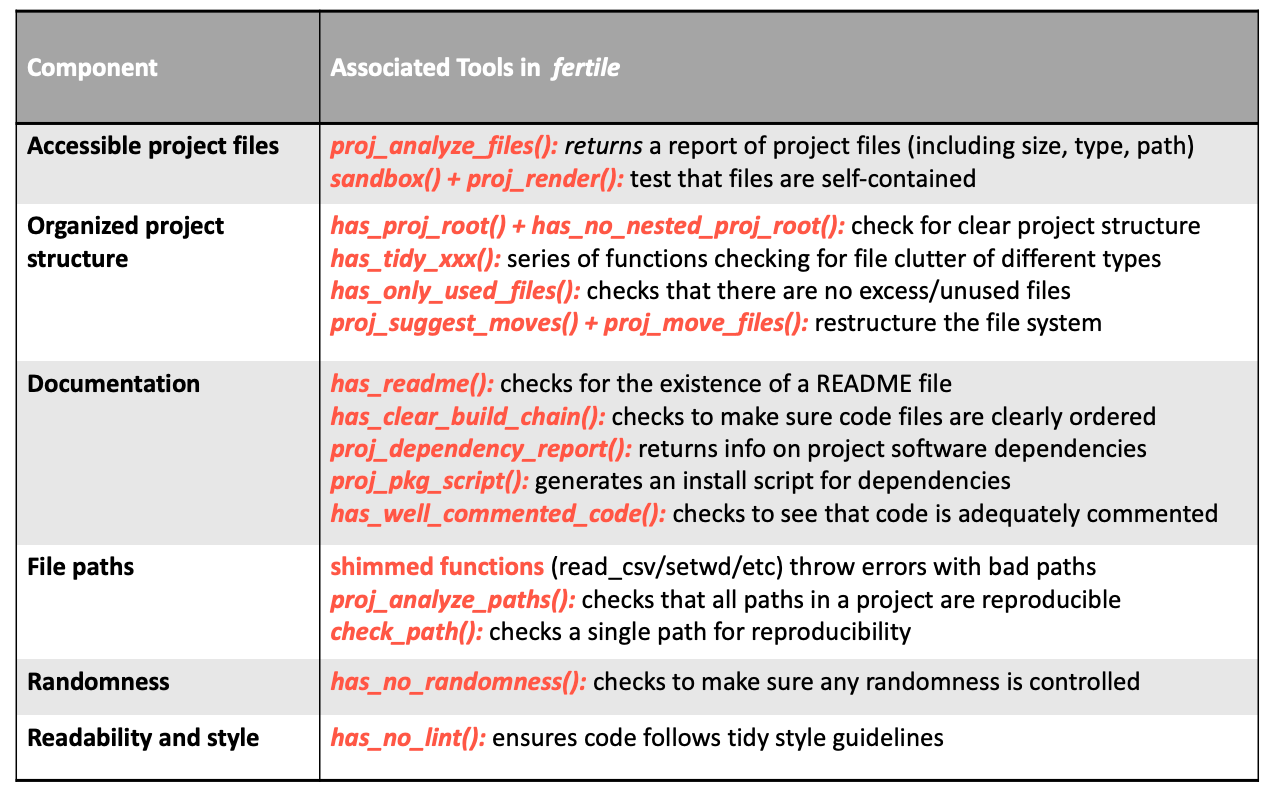
\includegraphics[width=1\linewidth]{figure/components-summary} \caption{Summary of Reproducibility Components and the Related Functionalities in 'fertile'}\label{fig:unnamed-chunk-48}
\end{figure}
\hypertarget{user-customizability}{%
\subsection{User Customizability}\label{user-customizability}}

\texttt{fertile} does not force its users into a box, instead allowing for a great deal of user choice in terms of which aspects of reproducibility to focus on. Users can run reproducibility tests at three different scales:
\begin{enumerate}
\def\labelenumi{\arabic{enumi})}
\item
  Comprehensively, where all checks are run within a single function or two.
\item
  In groups, where functions focused on similar aspects of reproducibility are run together.
\item
  Individually, where only one reproducbility check is run at a time.
\end{enumerate}
\hypertarget{comprehensive-features}{%
\subsubsection{Comprehensive Features}\label{comprehensive-features}}

Users who want comprehensive behavior can access it through three primary functions: \texttt{proj\_check()}, \texttt{proj\_analyze()}, and \texttt{proj\_badges()}.

The \texttt{proj\_check()} function runs all sixteen reproducibility tests in the package, noting which ones passed, which ones failed, the reason for failure, a recommended solution, and a guide to where to look for help. These tests, many of which were described in detail previously, include: looking for a clear build chain, checking to make sure the root level of the project is clear of clutter, confirming that there are no files present that are not being directly used by or created by the code, and looking for uses of randomness that do not have a call to \texttt{set.seed()} present. A full list is provided below:
\begin{Shaded}
\begin{Highlighting}[]
\FunctionTok{list\_checks}\NormalTok{()}
\end{Highlighting}
\end{Shaded}
\begin{verbatim}
-- The available checks in `fertile` are as follows: ------- fertile 1.1.9003 --
\end{verbatim}
\begin{verbatim}
 [1] "has_tidy_media"          "has_tidy_images"        
 [3] "has_tidy_code"           "has_tidy_raw_data"      
 [5] "has_tidy_data"           "has_tidy_scripts"       
 [7] "has_readme"              "has_no_lint"            
 [9] "has_proj_root"           "has_no_nested_proj_root"
[11] "has_only_used_files"     "has_clear_build_chain"  
[13] "has_no_absolute_paths"   "has_only_portable_paths"
[15] "has_no_randomness"       "has_well_commented_code"
\end{verbatim}
The \texttt{proj\_analyze()} function creates a report documenting the structure of a data analysis project, combining four key functions from \texttt{fertile} into one complete unit:
\begin{itemize}
\tightlist
\item
  \texttt{proj\_analyze\_packages()}, which captures a list of all packages referenced in the source code and which files they were referenced in
\item
  \texttt{proj\_analyze\_files()}, which captures a list of all of the files located in the directory along with their type and size
\item
  \texttt{proj\_suggest\_moves()}, which provides suggestions for how to reorganize files to create a more reproducible file structure
\item
  \texttt{proj\_analyze\_paths()}, which captures a list of the non-reproducible file paths referenced in source code
\end{itemize}
When \texttt{proj\_analyze()} is run on \texttt{project\_miceps}, we see the following information:
\begin{itemize}
\tightlist
\item
  10 packages (including \texttt{broom}, \texttt{dplyr}, \texttt{fs} and more) are referenced in the analysis code.
\item
  12 files are in the project directory, including some image files, data files, and a few files produced from some of the analyses that have been run by fertile (\texttt{install\_proj\_packages.R} and \texttt{software-versions.txt}).
\item
  There are 10 suggestions for moving files, with data files to \texttt{data-raw}, script files to \texttt{R}, and other files to \texttt{inst}.
\end{itemize}
\begin{Shaded}
\begin{Highlighting}[]
\FunctionTok{proj\_analyze}\NormalTok{(}\StringTok{\textquotesingle{}project\_miceps\textquotesingle{}}\NormalTok{)}
\end{Highlighting}
\end{Shaded}
\footnotesize
\begin{verbatim}
# A tibble: 10 x 3
   package       N used_in                    
   <chr>     <int> <chr>                      
 1 broom         1 project_miceps/analysis.Rmd
 2 dplyr         1 project_miceps/analysis.Rmd
 3 fs            1 project_miceps/analysis.Rmd
 4 ggplot2       1 project_miceps/analysis.Rmd
 5 purrr         1 project_miceps/analysis.Rmd
 6 readr         1 project_miceps/analysis.Rmd
 7 rmarkdown     1 project_miceps/analysis.Rmd
 8 skimr         1 project_miceps/analysis.Rmd
 9 stargazer     1 project_miceps/analysis.Rmd
10 tidyr         1 project_miceps/analysis.Rmd
# A tibble: 12 x 4
   file               ext        size mime                                      
   <fs::path>         <chr> <fs::byt> <chr>                                     
 1 Estrogen_Receptor~ docx     10.97K application/vnd.openxmlformats-officedocu~
 2 citrate_v_time.png png     187.02K image/png                                 
 3 proteins_v_time.p~ png     378.29K image/png                                 
 4 Blot_data_updated~ csv      14.43K text/csv                                  
 5 CS_data_redone.csv csv       7.39K text/csv                                  
 6 mice.csv           csv      14.33K text/csv                                  
 7 analysis.html      html      1.41M text/html                                 
 8 README.md          md           39 text/markdown                             
 9 install_proj_pack~ R           260 text/plain                                
10 software-versions~ txt       5.34K text/plain                                
11 miceps.Rproj       Rproj       204 text/rstudio                              
12 analysis.Rmd       Rmd       5.21K text/x-markdown                           
# A tibble: 10 x 3
   path_rel           dir_rel    cmd                                            
   <fs::path>         <fs::path> <chr>                                          
 1 Blot_data_updated~ data-raw   file_move('project_miceps/Blot_data_updated.cs~
 2 CS_data_redone.csv data-raw   file_move('project_miceps/CS_data_redone.csv',~
 3 Estrogen_Receptor~ inst/other file_move('project_miceps/Estrogen_Receptors.d~
 4 analysis.Rmd       vignettes  file_move('project_miceps/analysis.Rmd', fs::d~
 5 analysis.html      inst/text  file_move('project_miceps/analysis.html', fs::~
 6 citrate_v_time.png inst/image file_move('project_miceps/citrate_v_time.png',~
 7 install_proj_pack~ R          file_move('project_miceps/install_proj_package~
 8 mice.csv           data-raw   file_move('project_miceps/mice.csv', fs::dir_c~
 9 proteins_v_time.p~ inst/image file_move('project_miceps/proteins_v_time.png'~
10 software-versions~ inst/text  file_move('project_miceps/software-versions.tx~
NULL
\end{verbatim}
\normalsize

Similar to \texttt{proj\_check()}, \texttt{proj\_badges()} runs all sixteen reproducibility checks. However, the way the function displays the resulting information is different. Rather than report the results of each check individually alongside detailed information about why each failed, \texttt{proj\_badges()} provides a higher level summary, reporting on the \emph{groups} of checks that either passed or failed.

In \texttt{proj\_badges()}, the reproducibility checks are grouped into six categories corresponding to the six major components of reproducibility (see Figure 2.4 on the next page).

Each of the six badged has a set of \texttt{fertile} checks associated with it:
\begin{itemize}
\tightlist
\item
  Project Structure
  \begin{itemize}
  \tightlist
  \item
    \texttt{has\_proj\_root()}
  \item
    \texttt{has\_no\_nested\_proj\_root()}
  \end{itemize}
\item
  Tidy Files
  \begin{itemize}
  \tightlist
  \item
    \texttt{has\_tidy} \ldots{} \texttt{\_media()}, \texttt{\_images()}, \texttt{\_code()}, \texttt{\_raw\_data()}, \texttt{\_data()}, \texttt{\_scripts()}, \texttt{\_used\_files()}
  \end{itemize}
\item
  Documentation
  \begin{itemize}
  \tightlist
  \item
    \texttt{has\_readme()}
  \item
    \texttt{has\_clear\_build\_chain()}
  \item
    \texttt{has\_well\_commented\_code()}
  \end{itemize}
\item
  File Paths
  \begin{itemize}
  \tightlist
  \item
    \texttt{has\_no\_absolute\_paths()}
  \item
    \texttt{has\_only\_portable\_paths()}
  \end{itemize}
\item
  Randomness
  \begin{itemize}
  \tightlist
  \item
    \texttt{has\_no\_randomness()}
  \end{itemize}
\item
  Code Style
  \begin{itemize}
  \tightlist
  \item
    \texttt{has\_no\_lint()}
  \end{itemize}
\end{itemize}
When a user's project passes all of the checks associated with one of the categories, the user receives a badge certifying their success in that area. If it passes any fewer than \emph{all} available checks in a category, then the user fails to receive the corresponding badge.
\begin{figure}
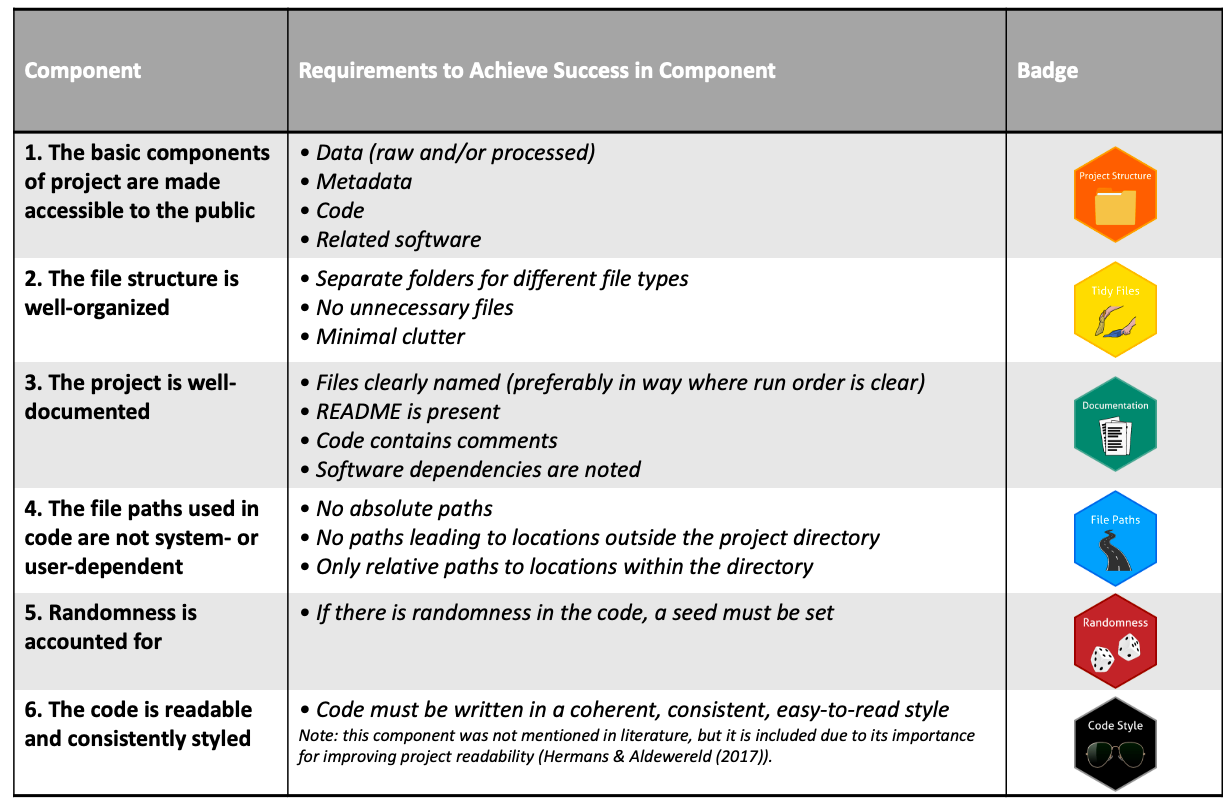
\includegraphics[width=1\linewidth]{figure/components-badges} \caption{The Six Components of Reproducibility Alongside Their Corresponding Badges}\label{fig:unnamed-chunk-50}
\end{figure}
\texttt{proj\_badges()} identifies the badges that a data analysis project should receive and then outputs a summary of this information---in the form of an \texttt{html} document---to the RStudio \texttt{Viewer} pane. This document---designed to produce a summary of a project that can be easily shared in places outside of \texttt{RStudio} (unlike the summaries produced by most other functions, which just produce output in the \texttt{R} console)---contains the following primary pieces of information:
\begin{enumerate}
\def\labelenumi{\arabic{enumi}.}
\item
  The name of the folder where the project is stored.
\item
  The reproducibility badges awarded to the project.
\item
  The reproducibility badges failed by the project.
\item
  If failures occurred, the reasons why. These are broken down by badge and list the checks associated with that badge that did not pass.
\item
  A date/time/timezone stamp of when the \texttt{html} summary was created.
\item
  Information about the user who generated the \texttt{html} summary (their full name, computer username, email, and GitHub username, if available).
\item
  Information about the \texttt{R} version, platform, and operating system of the computer used to generate the \texttt{html} at the time that it was created.
\item
  The names of files in the project that the \texttt{html} found the badges for as well as their date of last modification.
\end{enumerate}
The \texttt{html} output for \texttt{project\_miceps} can be seen below. As we can see, \texttt{project\_miceps} receives the ``Project Structure'' badge but fails ``Paths,'' ``Tidy Files,'' ``Documentation,'' ``Randomness,'' and ``Code Style.'' This aligns with our previous results from each of the components of reproducibility. For example, \texttt{project\_miceps} passed \texttt{has\_no\_nested\_proj\_root()} with flying colors, but failed \texttt{has\_well\_commented\_code()} (documentation), \texttt{has\_no\_randomness()} (randomness), and \texttt{has\_no\_lint()} (code style).

We see these failures reflected in the badge report section titled ``Reasons for Failure,'' which provides the list of functions responsible for why the project failed to receive that badge. For example, we can see that for the ``Tidy Files'' badge, \texttt{project\_miceps} failed \texttt{has\_tidy\_images()}, \texttt{has\_tidy\_raw\_data()}, and \texttt{has\_only\_used\_files()}.

At the end of the report, in the section titled ``Output Generation Details,'' we see information similar to what was produced with the previously described dependency management functions. We see the date the project was rendered by me, Audrey Bertin, on April 23rd, 2021 at around 10am eastern time using R version 4.0.4 on a Mac computer running macOS Big Sur. Additionally, we see the files contained in the project and their last modified dates.
\begin{figure}
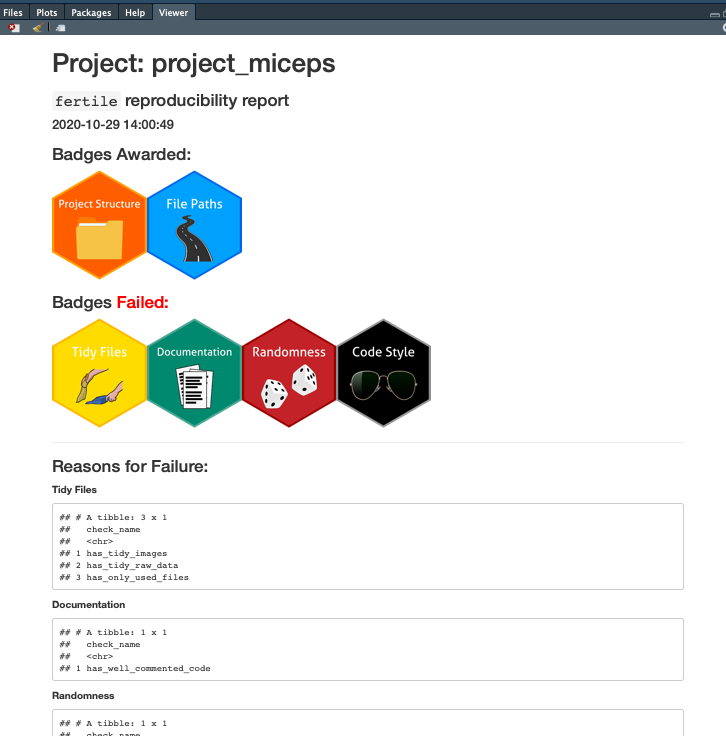
\includegraphics[width=1\linewidth]{figure/badges-1} \caption{Output: Badges and Reasons for Failure}\label{fig:badges-1}
\end{figure}
\begin{figure}
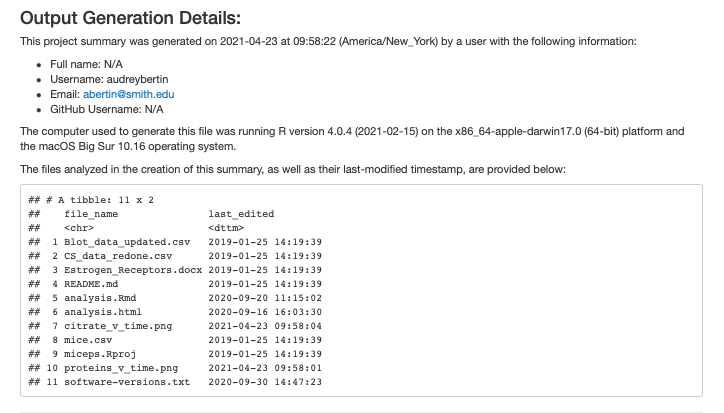
\includegraphics[width=1\linewidth]{figure/badges-2} \caption{Output: System/User Information and File List}\label{fig:badges-2}
\end{figure}
Together, \texttt{proj\_check()}, \texttt{proj\_analyze()}, and \texttt{proj\_badges()} cover a significant portion of all six major components of reproducibility.

\hypertarget{features-allowing-for-summary-by-group}{%
\subsubsection{Features Allowing For Summary By Group}\label{features-allowing-for-summary-by-group}}

Users wanting to focus on groups of checks can do so using the \texttt{proj\_check\_some()} or \texttt{proj\_check\_badge()} functions.

\texttt{proj\_check\_some()} leverages helper functions from \texttt{tidyselect} (Henry \& Wickham (2020)) to allow users to call groups of similar checks together. \texttt{tidyselect} helpers tell \texttt{fertile} to call only the checks whose names meet certain conditions. The helper functions that can be passed to \texttt{proj\_check\_some()} are:
\begin{itemize}
\tightlist
\item
  \texttt{starts\_with()}: Starts with a prefix.
\item
  \texttt{ends\_with()}: Ends with a suffix.
\item
  \texttt{contains()}: Contains a literal string.
\item
  \texttt{matches()}: Matches a regular expression.
\end{itemize}
For example, a variety of checks in \texttt{fertile} focus on making sure the project has a ``tidy'' structure--essentially that there are not files cluttered together all in one folder. Users interested in checking their tidyness can do so all at once using \texttt{proj\_check\_some()} as follows. When run on \texttt{project\_miceps}, we see that three of the tidyness checks fail, while three pass. The errors are associated with tidy scripts, image files, and data files.
\begin{Shaded}
\begin{Highlighting}[]
\FunctionTok{proj\_check\_some}\NormalTok{(}\StringTok{"project\_miceps"}\NormalTok{, }\FunctionTok{contains}\NormalTok{(}\StringTok{"tidy"}\NormalTok{))}
\end{Highlighting}
\end{Shaded}
\footnotesize
\begin{verbatim}
-- Running reproducibility checks -------------------------- fertile 1.1.9003 --
\end{verbatim}
\begin{verbatim}
v Checking for no *.R scripts at root level
\end{verbatim}
\begin{verbatim}
v Checking for no *.rda files at root level
\end{verbatim}
\begin{verbatim}
v Checking for no A/V files at root level
\end{verbatim}
\begin{verbatim}
* Checking for no image files at root level
\end{verbatim}
\begin{verbatim}
   Problem: Image files in root directory clutter project
\end{verbatim}
\begin{verbatim}
   Solution: Move source files to img/ directory
\end{verbatim}
\begin{verbatim}
   See for help: ?fs::file_move
\end{verbatim}
\begin{verbatim}
# A tibble: 2 x 2
  culprit                     expr                                              
  <fs::path>                  <glue>                                            
1 project_miceps/citrate_v_t~ fs::file_move('project_miceps/citrate_v_time.png'~
2 project_miceps/proteins_v_~ fs::file_move('project_miceps/proteins_v_time.png~
\end{verbatim}
\begin{verbatim}
* Checking for no raw data files at root level
\end{verbatim}
\begin{verbatim}
   Problem: Raw data files in root directory clutter project
\end{verbatim}
\begin{verbatim}
   Solution: Move raw data files to data-raw/ directory
\end{verbatim}
\begin{verbatim}
   See for help: ?fs::file_move
\end{verbatim}
\begin{verbatim}
# A tibble: 3 x 2
  culprit                     expr                                              
  <fs::path>                  <glue>                                            
1 project_miceps/Blot_data_u~ fs::file_move('project_miceps/Blot_data_updated.c~
2 project_miceps/CS_data_red~ fs::file_move('project_miceps/CS_data_redone.csv'~
3 project_miceps/mice.csv     fs::file_move('project_miceps/mice.csv', here::he~
\end{verbatim}
\begin{verbatim}
v Checking for no source files at root level
\end{verbatim}
\begin{verbatim}
-- Summary of fertile checks ------------------------------- fertile 1.1.9003 --
\end{verbatim}
\begin{verbatim}
v Reproducibility checks passed: 4
\end{verbatim}
\begin{verbatim}
* Reproducibility checks to work on: 2
\end{verbatim}
\begin{verbatim}
* Checking for no image files at root level
\end{verbatim}
\begin{verbatim}
   Problem: Image files in root directory clutter project
\end{verbatim}
\begin{verbatim}
   Solution: Move source files to img/ directory
\end{verbatim}
\begin{verbatim}
   See for help: ?fs::file_move
\end{verbatim}
\begin{verbatim}
# A tibble: 2 x 2
  culprit                     expr                                              
  <fs::path>                  <glue>                                            
1 project_miceps/citrate_v_t~ fs::file_move('project_miceps/citrate_v_time.png'~
2 project_miceps/proteins_v_~ fs::file_move('project_miceps/proteins_v_time.png~
\end{verbatim}
\begin{verbatim}
* Checking for no raw data files at root level
\end{verbatim}
\begin{verbatim}
   Problem: Raw data files in root directory clutter project
\end{verbatim}
\begin{verbatim}
   Solution: Move raw data files to data-raw/ directory
\end{verbatim}
\begin{verbatim}
   See for help: ?fs::file_move
\end{verbatim}
\begin{verbatim}
# A tibble: 3 x 2
  culprit                     expr                                              
  <fs::path>                  <glue>                                            
1 project_miceps/Blot_data_u~ fs::file_move('project_miceps/Blot_data_updated.c~
2 project_miceps/CS_data_red~ fs::file_move('project_miceps/CS_data_redone.csv'~
3 project_miceps/mice.csv     fs::file_move('project_miceps/mice.csv', here::he~
\end{verbatim}
\normalsize

Users might also attempt to call the two checks involving project roots together. When we do this, we see that \texttt{project\_miceps} has no issues with project roots and has a good root structure.
\begin{Shaded}
\begin{Highlighting}[]
\FunctionTok{proj\_check\_some}\NormalTok{(}\StringTok{"project\_miceps"}\NormalTok{, }\FunctionTok{ends\_with}\NormalTok{(}\StringTok{"root"}\NormalTok{))}
\end{Highlighting}
\end{Shaded}
\footnotesize
\begin{verbatim}
-- Running reproducibility checks -------------------------- fertile 1.1.9003 --
\end{verbatim}
\begin{verbatim}
v Checking for nested .Rproj files within project
\end{verbatim}
\begin{verbatim}
v Checking for single .Rproj file at root level
\end{verbatim}
\begin{verbatim}
-- Summary of fertile checks ------------------------------- fertile 1.1.9003 --
\end{verbatim}
\begin{verbatim}
v Reproducibility checks passed: 2
\end{verbatim}
\normalsize

\texttt{proj\_check\_badge()} is similar. It also allows users to run checks in groups, but these are not called by similar names, but rather based on which of the six components of reproducibility they belong to. This is done via a \texttt{badge} argument. Users input the shorthand name of the badge they want to run the checks for---e.g.~``randomness,'' ``paths,'' ``structure,'' etc.---and \texttt{fertile} then executes the corresponding functions.

For instance, if a user wants to run all of the checks associated with documentation, they would run the following code:
\begin{Shaded}
\begin{Highlighting}[]
\FunctionTok{proj\_check\_badge}\NormalTok{(}\StringTok{"project\_miceps"}\NormalTok{, }\StringTok{"documentation"}\NormalTok{)}
\end{Highlighting}
\end{Shaded}
\begin{verbatim}
v Checking for clear build chain
\end{verbatim}
\begin{verbatim}
v Checking for README file(s) at root level
\end{verbatim}
\begin{verbatim}
* Checking that code is adequately commented
\end{verbatim}
\begin{verbatim}
   Problem: Suboptimally commented .R or .Rmd files found
\end{verbatim}
\begin{verbatim}
   Solution: Add more comments to the files below. At least 10% of the lines should be comments.
\end{verbatim}
\begin{verbatim}
   See for help: https://intelligea.wordpress.com/2013/06/30/inline-and-block-comments-in-r/
\end{verbatim}
\begin{verbatim}
# A tibble: 1 x 2
  file_name                   fraction_lines_commented
  <chr>                                          <dbl>
1 project_miceps/analysis.Rmd                     0.04
\end{verbatim}
\begin{verbatim}
-- Summary of fertile checks ------------------------------- fertile 1.1.9003 --
\end{verbatim}
\begin{verbatim}
v Reproducibility checks passed: 2
\end{verbatim}
\begin{verbatim}
* Reproducibility checks to work on: 1
\end{verbatim}
\begin{verbatim}
* Checking that code is adequately commented
\end{verbatim}
\begin{verbatim}
   Problem: Suboptimally commented .R or .Rmd files found
\end{verbatim}
\begin{verbatim}
   Solution: Add more comments to the files below. At least 10% of the lines should be comments.
\end{verbatim}
\begin{verbatim}
   See for help: https://intelligea.wordpress.com/2013/06/30/inline-and-block-comments-in-r/
\end{verbatim}
\begin{verbatim}
# A tibble: 1 x 2
  file_name                   fraction_lines_commented
  <chr>                                          <dbl>
1 project_miceps/analysis.Rmd                     0.04
\end{verbatim}
As can be seen above, this outputs the results from the following \texttt{fertile} checks involving documentation:
\begin{itemize}
\tightlist
\item
  \texttt{has\_clear\_build\_chain()}
\item
  \texttt{has\_readme()}
\item
  \texttt{has\_well\_commented\_code()}
\end{itemize}
A user who wanted to check \texttt{project\_miceps} for tidyness instead would run the same function, but changing out the second argument from ``documentation'' to ``tidy-files'':
\begin{Shaded}
\begin{Highlighting}[]
\FunctionTok{proj\_check\_badge}\NormalTok{(}\StringTok{"project\_miceps"}\NormalTok{, }\StringTok{"tidy{-}files"}\NormalTok{)}
\end{Highlighting}
\end{Shaded}
\begin{verbatim}
Joining, by = "path_abs"
\end{verbatim}
\begin{verbatim}
v Checking for no *.R scripts at root level
\end{verbatim}
\begin{verbatim}
v Checking for no *.rda files at root level
\end{verbatim}
\begin{verbatim}
v Checking for no A/V files at root level
\end{verbatim}
\begin{verbatim}
* Checking for no image files at root level
\end{verbatim}
\begin{verbatim}
   Problem: Image files in root directory clutter project
\end{verbatim}
\begin{verbatim}
   Solution: Move source files to img/ directory
\end{verbatim}
\begin{verbatim}
   See for help: ?fs::file_move
\end{verbatim}
\begin{verbatim}
# A tibble: 2 x 2
  culprit                     expr                                              
  <fs::path>                  <glue>                                            
1 project_miceps/citrate_v_t~ fs::file_move('project_miceps/citrate_v_time.png'~
2 project_miceps/proteins_v_~ fs::file_move('project_miceps/proteins_v_time.png~
\end{verbatim}
\begin{verbatim}
* Checking for no raw data files at root level
\end{verbatim}
\begin{verbatim}
   Problem: Raw data files in root directory clutter project
\end{verbatim}
\begin{verbatim}
   Solution: Move raw data files to data-raw/ directory
\end{verbatim}
\begin{verbatim}
   See for help: ?fs::file_move
\end{verbatim}
\begin{verbatim}
# A tibble: 3 x 2
  culprit                     expr                                              
  <fs::path>                  <glue>                                            
1 project_miceps/Blot_data_u~ fs::file_move('project_miceps/Blot_data_updated.c~
2 project_miceps/CS_data_red~ fs::file_move('project_miceps/CS_data_redone.csv'~
3 project_miceps/mice.csv     fs::file_move('project_miceps/mice.csv', here::he~
\end{verbatim}
\begin{verbatim}
v Checking for no source files at root level
\end{verbatim}
\begin{verbatim}
* Checking to see if all files in directory are used in code
\end{verbatim}
\begin{verbatim}
   Problem: You have files in your project directory which are not being used.
\end{verbatim}
\begin{verbatim}
   Solution: Use or delete files.
\end{verbatim}
\begin{verbatim}
   See for help: ?fs::file_delete
\end{verbatim}
\begin{verbatim}
# A tibble: 2 x 1
  path_abs                                                                      
  <chr>                                                                         
1 /Users/audreybertin/Documents/thesis/index/project_miceps/Estrogen_Receptors.~
2 /Users/audreybertin/Documents/thesis/index/project_miceps/mice.csv            
\end{verbatim}
\begin{verbatim}
-- Summary of fertile checks ------------------------------- fertile 1.1.9003 --
\end{verbatim}
\begin{verbatim}
v Reproducibility checks passed: 4
\end{verbatim}
\begin{verbatim}
* Reproducibility checks to work on: 3
\end{verbatim}
\begin{verbatim}
* Checking for no image files at root level
\end{verbatim}
\begin{verbatim}
   Problem: Image files in root directory clutter project
\end{verbatim}
\begin{verbatim}
   Solution: Move source files to img/ directory
\end{verbatim}
\begin{verbatim}
   See for help: ?fs::file_move
\end{verbatim}
\begin{verbatim}
# A tibble: 2 x 2
  culprit                     expr                                              
  <fs::path>                  <glue>                                            
1 project_miceps/citrate_v_t~ fs::file_move('project_miceps/citrate_v_time.png'~
2 project_miceps/proteins_v_~ fs::file_move('project_miceps/proteins_v_time.png~
\end{verbatim}
\begin{verbatim}
* Checking for no raw data files at root level
\end{verbatim}
\begin{verbatim}
   Problem: Raw data files in root directory clutter project
\end{verbatim}
\begin{verbatim}
   Solution: Move raw data files to data-raw/ directory
\end{verbatim}
\begin{verbatim}
   See for help: ?fs::file_move
\end{verbatim}
\begin{verbatim}
# A tibble: 3 x 2
  culprit                     expr                                              
  <fs::path>                  <glue>                                            
1 project_miceps/Blot_data_u~ fs::file_move('project_miceps/Blot_data_updated.c~
2 project_miceps/CS_data_red~ fs::file_move('project_miceps/CS_data_redone.csv'~
3 project_miceps/mice.csv     fs::file_move('project_miceps/mice.csv', here::he~
\end{verbatim}
\begin{verbatim}
* Checking to see if all files in directory are used in code
\end{verbatim}
\begin{verbatim}
   Problem: You have files in your project directory which are not being used.
\end{verbatim}
\begin{verbatim}
   Solution: Use or delete files.
\end{verbatim}
\begin{verbatim}
   See for help: ?fs::file_delete
\end{verbatim}
\begin{verbatim}
# A tibble: 2 x 1
  path_abs                                                                      
  <chr>                                                                         
1 /Users/audreybertin/Documents/thesis/index/project_miceps/Estrogen_Receptors.~
2 /Users/audreybertin/Documents/thesis/index/project_miceps/mice.csv            
\end{verbatim}
This runs all of the checks associated with ensuring that there is minimal file clutter: the six checks starting with \texttt{has\_tidy\_}, alongside \texttt{has\_only\_used\_files()}.

\hypertarget{individual-checks}{%
\subsubsection{Individual Checks}\label{individual-checks}}

If users do not want to run functions in groups, and prefer to run them individually, that option is also provided to them. Every check that makes up \texttt{check()} and every sub-component of \texttt{project\_analyze()}can be run individually.

\hypertarget{educational-features}{%
\subsection{Educational Features}\label{educational-features}}

Simply noting and correcting issues with reproducibility is not enough to produce lasting change in the scientific community. Data analysts and software users must also be educated on why their choices were not reproducible so that they do not fall victim to those mistakes again in the future, but also so that they can share their knowledge and experience with others in the scientific community.

\texttt{fertile} prioritizes this idea of reproducibility education throughout many of its functionalities.

One of the major ways through which \texttt{fertile} educates is users is a system of command tracking and interactive messaging. As long as \texttt{fertile} is loaded in \texttt{R}, the package records when commands that have the potential to affect reproducibility are run in the console.

As soon as a dangerous function is called, \texttt{fertile} alerts the user and provides suggestions for alternative solutions. This behavior, explained in more detail in Chapter 2.2.4, gives users immediate feedback on their behavior. In addition to assisting users in the moment, this method has also been shown to increase long-run retention of information when compared with feedback after the fact (Epstein et al. (2002)).

Users interested in looking back at their past choices can do so as well. The \texttt{log\_report()} function provides access to a log listing the commands with a link to reproducibility that have been called.

When we execute the commands \texttt{library(purrr)}, \texttt{library(forcats)}, and \texttt{read\_csv(fs::path(\textquotesingle{}project\_miceps\textquotesingle{},\ "mice.csv"))}, we see those actions appear in the log. Since \texttt{read\_csv} takes a file path argument, \texttt{fertile} captures the path that was called and reports it under \texttt{path}.
\begin{Shaded}
\begin{Highlighting}[]
\FunctionTok{log\_report}\NormalTok{()}
\end{Highlighting}
\end{Shaded}
\footnotesize
\begin{verbatim}
Reading from /Users/audreybertin/Documents/thesis/index/.fertile_log.csv
\end{verbatim}
\begin{verbatim}
# A tibble: 1,566 x 4
   path            path_abs                        func      timestamp          
   <chr>           <chr>                           <chr>     <dttm>             
 1 package:remotes <NA>                            base::re~ 2020-09-20 15:20:34
 2 package:thesis~ <NA>                            base::re~ 2020-09-20 15:20:34
 3 package:thesis~ <NA>                            base::li~ 2020-09-20 15:20:34
 4 package:stringr <NA>                            base::li~ 2020-09-21 13:28:29
 5 package:fertile <NA>                            base::li~ 2020-09-21 13:28:29
 6 ~/Desktop/my_d~ ~/Desktop/my_data.csv           utils::r~ 2020-09-21 13:28:29
 7 ../../../Deskt~ /Users/audreybertin/Desktop/my~ utils::r~ 2020-09-21 13:28:29
 8 package:purrr   <NA>                            base::li~ 2020-09-21 13:28:36
 9 package:forcats <NA>                            base::li~ 2020-09-21 13:28:36
10 project_miceps~ /Users/audreybertin/Documents/~ readr::r~ 2020-09-21 13:28:36
# ... with 1,556 more rows
\end{verbatim}
\normalsize

Depending on how much history they want to keep track of, users have the option to clear the log and start from scratch via the function \texttt{log\_clear()}.

In addition to this educational logging behavior, the reproducibility checks contained in the \texttt{check()} function also include educational messages. We consider several examples below:
\begin{itemize}
\item
  \texttt{has\_no\_randomness()}, when it fails, tells users that their code uses randomness and they should use the \texttt{set.seed()} function to control it.
\item
  \texttt{has\_only\_used\_files()}, when it fails, tells users that there are files present in the directory not being used for any purpose and provides a function (\texttt{fs::file\_delete}) to use in order to remove them.
\item
  \texttt{has\_no\_lint()}, when it fails, provides users a list of all of the ways in which their code fails to follow tidy style and points them to the exact lines and characters in the code where the mistakes occurred.
\item
  \texttt{has\_tidy\_images}, when it fails, tells users that it has found files in the root directory which add clutter and recommends that they be moved to an \texttt{img/} directory.
\end{itemize}
Users are provided with an informative message about their issue but are not always provided a fully automated solution. This behavior encourages them to learn as they have to execute the suggested solution themselves.

However, even though \texttt{fertile} often requires users to take their own actions, that does not mean that the package requires users to be of high skill level to use. \texttt{fertile} is designed in such a way so its educational benefits can be achieved with relative simplicity and minimal effort so that even users brand new to \texttt{R} can gain knowledge and awareness of reproducibility from using it.

For example, the interactive messaging features require no effort beyond the loading of the package with \texttt{library(fertile)} to activate. And many of the educational benefits contained within the checks can be gained all at once as well, with a single call of the \texttt{check()} function. Users looking for more customizability have the option to go into more detail with the more complex functions like \texttt{sandbox()}, but they are not necessary for users to gain benefit from the package.

\hypertarget{how-fertile-works}{%
\section{\texorpdfstring{How \texttt{fertile} Works}{How fertile Works}}\label{how-fertile-works}}

In the world of \texttt{R} packages, \texttt{fertile}`s behavior is rather unusual. Few packages manipulate their users' \texttt{R} environments or file structure, instead remaining relatively self-contained. This unique behavior necessitates the use of several non-traditional techniques, described below.

\hypertarget{shims}{%
\subsection{Shims}\label{shims}}

Much of the functionality in \texttt{fertile} is achieved by writing \texttt{shims}. In their application to \texttt{fertile}, shims can be defined as functions that transparently intercept users' intended actions and slightly alter their execution.

\texttt{fertile} contains shims for a variety of common functions that may affect reproducibility, including those that read and write files, load libraries, and set random number generation seeds.

When users perform actions that may threaten reproducibility, the package's shimmed functions capture the user's commands, log their behavior, and check and report on file paths before proceeding to executing the desired function.

This allows \texttt{fertile} to warn users when they use a potentially non-reproducible file path and also helps keep track of past behavior via a log of previously entered commands.

The shim-writing process looks as follows:
\begin{enumerate}
\def\labelenumi{\arabic{enumi}.}
\item
  Identify an \texttt{R} function that is likely to be used in a way that may break reproducibility. For example, a function that reads in files.
\item
  Create a function in \texttt{fertile} with the same name that takes the same arguments.
\item
  Write this new function so that it:
  \begin{enumerate}
  \def\labelenumii{\alph{enumii})}
  \tightlist
  \item
    captures the specified arguments,
  \item
    logs the name of the function the user was intending to call,
  \item
    performs file path checks on any path-related arguments, and
  \item
    calls the original function with the original arguments.
  \end{enumerate}
\end{enumerate}
If the file path checks execute without error, the operation of a shim looks the same to the user as if they were calling the original function. However, if an error is thrown---i.e.~a path is found to be non-reproducible---then execution will stop before step \emph{d} is completed.

Most shims are relatively simple. Several, such as that for \texttt{library()} are more complex, but many follow the same basic format. Consider this example for \texttt{read.csv()}:
\begin{Shaded}
\begin{Highlighting}[]
\NormalTok{fertile}\SpecialCharTok{::}\NormalTok{read.csv}
\end{Highlighting}
\end{Shaded}
\begin{verbatim}
function(file, ...) {
  if (interactive_log_on()) {
    log_push(file, "utils::read.csv")
    check_path_safe(file, ... = "utils::read.csv")
    utils::read.csv(file, ...)
  }
}
<bytecode: 0x7f8028b3dde0>
<environment: namespace:fertile>
\end{verbatim}
This functionality all occurs without the knowledge of the user. Consider the example of \texttt{read.csv()}. \texttt{read.csv()} is a popular function from the \texttt{utils} package for reading in data files. Users with both \texttt{utils} and \texttt{fertile} loaded will experience the following: The user will call \texttt{read.csv()} as normal, thinking that they are calling \texttt{utils::read.csv()}. However, they will actually be calling \texttt{fertile::read.csv()}, a very similar function with the same name. \texttt{fertile::read.csv()} will then capture the file path the user provided and check whether it is reproducible. If it is deemed okay, the function will execute as intended and read in the data just as \texttt{utils::read.csv()} would. If it is deemed non-reproducible, the function will return an error telling the user to use an alternate file path. Either way, \texttt{fertile} will record that the user called \texttt{utils::read.csv()} and note the path that was provided to it for future reference.

This behavior, however, is dependent on \texttt{fertile} remaining at the top of the \texttt{search()} path so that its functions are called preferentially over the original functions that it has shimmed. In order to ensure that the \texttt{fertile} versions of functions (``shims'') always supersede (``mask'') their original namesakes when called, \texttt{fertile} uses its own shims of the \texttt{library} and \texttt{require} functions to manipulate the \texttt{R} \texttt{search} path so that it is always located in the first position.

In the \texttt{fertile} version of \texttt{library()}, \texttt{fertile} is detached from the search path, the requested package is loaded, and then \texttt{fertile} is reattached. This ensures that when a user executes a command, \texttt{R} will check \texttt{fertile} for a matching function before considering other packages.

A full list of the shimmed functions provided by \texttt{fertile} is included below. Note that in order to reduce the software dependencies of \texttt{fertile} the shims from the less common \texttt{readxl}, \texttt{rjson}, \texttt{foreign}, and \texttt{sas7bdat} packages are only activated if the user has those packages installed and loaded on their computer.
\begin{figure}
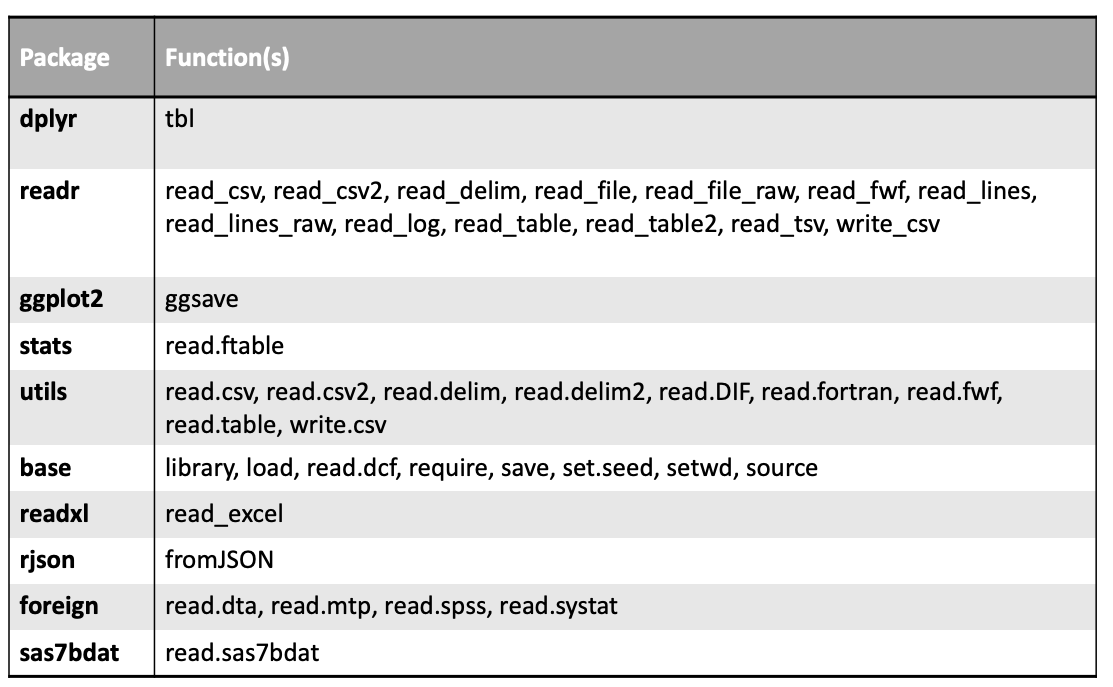
\includegraphics[width=1\linewidth]{figure/shims-list} \caption{List of Functions Shimmed by 'fertile'}\label{fig:unnamed-chunk-59}
\end{figure}
\hypertarget{shim-customization-functionality}{%
\subsubsection{Shim Customization Functionality}\label{shim-customization-functionality}}

Not all \texttt{R} programmers use the same packages, nor do they use the same functions at the same level of regularity. Additionally, some users might not always want to have their shimmed functions enabled---for example, they may purposefully be writing code with absolute paths, and would want to be able to do so without warnings and interruptions.

As a result of this, we believe it important to include features in \texttt{fertile} that enable users to customize which functions for which their version of \texttt{fertile} has active shims as well as when those shims are enabled or disabled.

Several functions in \texttt{fertile} have been written to implement this behavior:
\begin{enumerate}
\def\labelenumi{\arabic{enumi}.}
\tightlist
\item
  The \texttt{add\_shim()} function allows users to write a new shim to \texttt{fertile}. When this function is called, \texttt{fertile} writes the code for the shimmed function using the standard structure explained previously. It then adds that code to a file located alongside \texttt{fertile}'s documentation on the user's computer so that it is permanently saved, and then executes it in order to activate the new shim and immediately bring it into the user's \texttt{R} environment. With \texttt{add\_shim()}, users can only add shims individually, as in the example below, where a shim for the function \texttt{write.ftable} from the \texttt{stats} package is added.
\end{enumerate}
\begin{Shaded}
\begin{Highlighting}[]
\CommentTok{\# Code to add a shim for stats::write.ftable }
\FunctionTok{add\_shim}\NormalTok{(}\AttributeTok{func =} \StringTok{"write.ftable"}\NormalTok{, }\AttributeTok{package =} \StringTok{"stats"}\NormalTok{)}
\end{Highlighting}
\end{Shaded}
\begin{enumerate}
\def\labelenumi{\arabic{enumi}.}
\setcounter{enumi}{1}
\tightlist
\item
  If users want to not limit themselves to a handful of specific shims and rather just automatically create all of the possible shims, the \texttt{find\_all\_shimmable\_functions()}, \texttt{find\_pkg\_shimmable\_functions()} and \texttt{add\_all\_possible\_shims()} functions can assist.
\end{enumerate}
\texttt{find\_all\_shimmable\_functions()} searches the namespaces of all of the loaded libraries in \texttt{search()} and returns the names and associated packages of all functions found to potentially be shimmable (i.e.~those that appear to accept file path-related arguments). This list provides a reference for those who want to know which functions they could potentially write shims for.

\texttt{find\_pkg\_shimmable\_functions()} does the same thing as \texttt{find\_all\_shimmable\_}
\texttt{functions()}, but on a smaller scale. Rather than looking at all loaded packages, it just looks at the namespace of a specific package, passed as an argument to the user.

\texttt{add\_all\_possible\_shims()} will look at the list of functions provided by \texttt{find\_all\_shimmable\_functions()} and perform the actions of \texttt{add\_shim()} on all of them individually. This will generate and then add all of those functions to the shim file included alongside the \texttt{fertile} documentation and then load them into the environment.
\begin{Shaded}
\begin{Highlighting}[]
\CommentTok{\# Return list of all potential shims in ALL loaded packages}
\FunctionTok{find\_all\_shimmable\_functions}\NormalTok{()}
\end{Highlighting}
\end{Shaded}
\begin{Shaded}
\begin{Highlighting}[]
\CommentTok{\# Return list of all potential shims from a SPECIFIC package (e.g dplyr)}
\FunctionTok{library}\NormalTok{(dplyr)}
\end{Highlighting}
\end{Shaded}
\begin{verbatim}
Reading from /Users/audreybertin/Documents/thesis/index/.fertile_log.csv
\end{verbatim}
\begin{Shaded}
\begin{Highlighting}[]
\FunctionTok{find\_pkg\_shimmable\_functions}\NormalTok{(}\AttributeTok{package =} \StringTok{"dplyr"}\NormalTok{)}
\end{Highlighting}
\end{Shaded}
\begin{verbatim}
[1] "src_sqlite"
\end{verbatim}
\begin{Shaded}
\begin{Highlighting}[]
\CommentTok{\# Write/load all of the shims from find\_all\_shimmable\_functions()}
\FunctionTok{add\_all\_possible\_shims}\NormalTok{()}
\end{Highlighting}
\end{Shaded}
\begin{enumerate}
\def\labelenumi{\arabic{enumi}.}
\setcounter{enumi}{2}
\tightlist
\item
  By default, all of the shims in \texttt{fertile}---both those included in the package as well as those written by the user---are activated when \texttt{fertile} is loaded (using \texttt{library()}) and deactivated, i.e.~removed from the environment, when it is unloaded.
\end{enumerate}
There is no method currently in the package to deactivate the shims included in \texttt{fertile} without unloading it. However, the shims written by the user are completely controllable in this respect. \texttt{load\_shims()} will find the file of user generated shims and execute it to bring those shims into the environment. \texttt{unload\_shims()} will search the environment for functions that are linked to \texttt{fertile}, via unique attributes written into the functions, and remove them.
\begin{enumerate}
\def\labelenumi{\arabic{enumi}.}
\setcounter{enumi}{3}
\tightlist
\item
  Finally, users can edit the file containing the shims they have written using the function \texttt{edit\_shims()}. This will open an interactive window which provides the user with access to the file so that they can delete or reorganize shims as desired.
\end{enumerate}
\hypertarget{hidden-files}{%
\subsection{Hidden Files}\label{hidden-files}}

In order to store and analyze information about user behavior and code structure, \texttt{fertile} utilizes three different types of hidden files, two of which are \texttt{.csv} format and one of which is a text file. The hidden \texttt{.csv} files for \texttt{project\_miceps} can be seen below:
\begin{Shaded}
\begin{Highlighting}[]
\FunctionTok{as.character}\NormalTok{(}
\NormalTok{  fs}\SpecialCharTok{::}\FunctionTok{dir\_ls}\NormalTok{(}\StringTok{"project\_miceps"}\NormalTok{, }\AttributeTok{all =} \ConstantTok{TRUE}\NormalTok{, }\AttributeTok{glob =} \StringTok{"*\_log.csv"}\NormalTok{)}
\NormalTok{)}
\end{Highlighting}
\end{Shaded}
\begin{verbatim}
[1] "project_miceps/.fertile_log.csv"       
[2] "project_miceps/.fertile_render_log.csv"
\end{verbatim}
The interactive log (\texttt{.fertile\_log.csv}), accessible via \texttt{log\_report()}, is created as soon as a user executes their first piece of code that could threaten reproducibility. This file tracks all of the shimmed functions executed by the user, either in the console or when running code chunks by hand (rather than knitting a file). It reports the function called, the relevant argument passed in (either a file path or \texttt{R} package name), and the time stamp of when the function was executed. Users can clear the data from this file and start fresh at any time with \texttt{log\_clear()}.

The render log (\texttt{.fertile\_render\_log.csv}), accessible via \texttt{render\_log\_report()}, has a similar structure to the interactive log but is not under the control of the user. It tracks information about the code contained within \texttt{.R} and \texttt{.Rmd} files within the project a user is testing for reproducibility. A new render log file can be generated in one of three different ways:
\begin{enumerate}
\def\labelenumi{\arabic{enumi}.}
\item
  The first time a user runs one of the major reproducibility checks from \texttt{fertile}, such as \texttt{proj\_check()}, \texttt{proj\_analyze()}, or one of the smaller checks within that requires access to the contents of code files.
\item
  Any time a check involving code is called in \texttt{fertile}, the package checks to see whether any code files have been updated since the last time a render log was generated. If so, a new render log is generated.
\item
  The user can generate a new file manually at any time by executing the \texttt{proj\_render()} command.
\end{enumerate}
The render log contains information used to run many of the checks in \texttt{fertile}. It captures the random number generator seed before and after executing code, notes which packages and files are accessed and the function with which they were called, and contains a time stamp of the last time the code was run by \texttt{fertile}.

In the render log report for project miceps, we see calls to the packages that have previously been noted as dependencies (e.g.~\texttt{dplyr}, \texttt{readr}, \texttt{tidyr}, etc.), references to file paths in the code (e.g.~\texttt{Blot\_data\_updated.csv}), and a timestamp of the last render.
\begin{Shaded}
\begin{Highlighting}[]
\FunctionTok{render\_log\_report}\NormalTok{(}\StringTok{"project\_miceps"}\NormalTok{)}
\end{Highlighting}
\end{Shaded}
\footnotesize
\begin{verbatim}
# A tibble: 21 x 4
   path                    path_abs                  func    timestamp          
   <chr>                   <chr>                     <chr>   <dttm>             
 1 Seed @ Start            <NA>                      578     2021-05-17 23:10:26
 2 package:dplyr           <NA>                      base::~ 2021-05-17 23:10:26
 3 package:readr           <NA>                      base::~ 2021-05-17 23:10:26
 4 package:tidyr           <NA>                      base::~ 2021-05-17 23:10:27
 5 package:ggplot2         <NA>                      base::~ 2021-05-17 23:10:27
 6 package:purrr           <NA>                      base::~ 2021-05-17 23:10:27
 7 Seed Before             <NA>                      578     2021-05-17 23:10:27
 8 /Users/audreybertin/Do~ /Users/audreybertin/Docu~ readr:~ 2021-05-17 23:10:27
 9 Seed After              <NA>                      592     2021-05-17 23:10:27
10 Seed Before             <NA>                      592     2021-05-17 23:10:27
# ... with 11 more rows
\end{verbatim}
\normalsize

In addition to the two log files, \texttt{fertile} keeps a third hidden file to track project dependencies. Described in detail in the section on documentation, this file keeps track of the software setup that a project is run under. A new version is generated every time \texttt{fertile} compiles the project code files or when users request to view the file (via a special access function). Like the log files, however, there is no simple way to manually modify or delete the file, ensuring that it does not accidentally get changed in a way that would damage reproducibility.

\hypertarget{environment-variables}{%
\subsection{Environment Variables}\label{environment-variables}}

The shims in \texttt{fertile} are designed to be able to write to both the interactive and render logs. That way, no matter whether a user calls \texttt{read\_csv()} interactively or writes it in their code file, \texttt{fertile} will still take note of the fact that the action has happened.

Given the different purposes of each file, however, it is important that \texttt{fertile} be able to identify when a function execution should be saved to the interactive log versus when it should be saved to the render log.

This information is tracked via a logical environment variable---a variable whose value is stored in a user's local \texttt{R} environment, and whose value can be accessed or updated via commands---called \texttt{FERTILE\_RENDER\_MODE}. When \texttt{FERTILE\_RENDER\_MODE} is \texttt{TRUE}, executed shims are saved to the render log. When it is \texttt{FALSE}, they are saved to the interactive log.

Since \texttt{fertile} is designed to capture information about interactive user behavior, \texttt{FERTILE\_RENDER\_MODE} is \texttt{FALSE} by default. It is only changed to \texttt{TRUE} when \texttt{fertile} is executing functions that involve the rendering of \texttt{.R} and \texttt{.Rmd} code files. At the start of all such functions, \texttt{fertile} sets the environment variable to \texttt{TRUE}, executes the majority of the function, and then sets it back to \texttt{FALSE} before exiting. This ensures that as soon as the function has finished running, all new commands get executed on the interactive log, rather on the render log which was just generated.

The example of \texttt{has\_only\_portable\_paths()} illustrates this functionality. We see several clear steps to this function:
\begin{enumerate}
\def\labelenumi{\arabic{enumi}.}
\item
  The environment variable is set to \texttt{TRUE}, so that \texttt{fertile} knows to write any information about shimmed functions to the render log.
\item
  If a render log does not yet exist or the project has been updated since the last time one was generated, then the project is rendered with \texttt{proj\_render()}, generating a new render log.
\item
  This render log is read to find information about the file paths that were captured when executing the code files.
\item
  \texttt{fertile} checks to see if the paths are portable---meaning that they are both relative and point within the project directory---and outputs a a list of the ones that are not, if any, in addition to some information about how to correct that.
\item
  The environment variable is set back to \texttt{FALSE} so that interactive behavior is once again captured.
\end{enumerate}
\begin{Shaded}
\begin{Highlighting}[]
\NormalTok{has\_only\_portable\_paths}
\end{Highlighting}
\end{Shaded}
\begin{verbatim}
function(path = ".") {
  Sys.setenv("FERTILE_RENDER_MODE" = TRUE)

  check_is_dir(path)

  if (!has_rendered(path)) {
    proj_render(path)
  }

  paths <- log_report(path) %>%
    dplyr::filter(!grepl("package:", path)) %>%
    dplyr::pull(path)

  good <- paths %>%
    is_path_portable()

  errors <- tibble(
    culprit = as_fs_path(paths[!good]),
    expr = glue("fs::path_rel('{culprit}')")
  )

  Sys.setenv("FERTILE_RENDER_MODE" = FALSE)

  make_check(
    name = "Checking for only portable paths",
    state = all(good),
    problem = "Non-portable paths won't necessarily work for others",
    solution = "Use relative paths.",
    help = "?fs::path_rel",
    errors = errors
  )
}
<bytecode: 0x7f80251d9740>
<environment: namespace:fertile>
attr(,"req_compilation")
[1] TRUE
\end{verbatim}
\hypertarget{the-dots}{%
\subsection{The Dots (\ldots)}\label{the-dots}}

\texttt{fertile} utilizes the dots (\ldots) in shims, the file path messaging system, and the \texttt{proj\_check\_some()} function.

The dots are a mechanism built into \texttt{R} to allow for variability in the arguments passed to a function. They allow the user to pass in a variety of arguments to a function---in any number---rather than forcing them to pass in a set number. Additionally, the dots can be easily captured and passed on to another function.

These dots help \texttt{fertile} achieve its desired functionality in several ways.

Many of the shimmed functions in \texttt{fertile} accept a large number of arguments. Consider \texttt{read\_csv()}. The function requires only one argument (\texttt{file}) but allows for up to 14.
\begin{Shaded}
\begin{Highlighting}[]
\FunctionTok{formals}\NormalTok{(readr}\SpecialCharTok{::}\NormalTok{read\_csv)}
\end{Highlighting}
\end{Shaded}
\small
\begin{verbatim}
$file


$col_names
[1] TRUE

$col_types
NULL

$locale
default_locale()

$na
c("", "NA")

$quoted_na
[1] TRUE

$quote
[1] "\""

$comment
[1] ""

$trim_ws
[1] TRUE

$skip
[1] 0

$n_max
[1] Inf

$guess_max
min(1000, n_max)

$progress
show_progress()

$skip_empty_rows
[1] TRUE
\end{verbatim}
\normalsize

\texttt{read\_csv()} is not alone. Many functions like it have a large number of arguments. It would be a very cumbersome process to have to re-write all of them arguments by hand in each shim. Additionally, it would make the shim-writing process not very reproducible: if every shim took a lengthy list of arguments with all different names and types, which all had to be specified in the definition of each shim, it would be complicated to scale up the library of available shims! There would be no easy method to automate this process, so many would have to be written by hand.

When the dots are used, none of these problems arise. In a \texttt{fertile} shim, we only have to define the parameters that are required for the function being shimmed to operate---plus, of course, anything related to file paths---and then just say that everything else will go through the dots.

When a user executes a shim, anything passed through the path arguments gets evaluated for reproducibility and everything else is saved through the dots. Those dots then get handed over to the original function. This function knows what to do with them, because the user was running the \texttt{fertile} shim as if it were the original function, and therefore passed arguments that the original function could interpret.

In the \texttt{read\_csv()} example, we see that the \texttt{fertile} shim takes only \texttt{file} and \texttt{...} as arguments. Users can still pass any of the 14 \texttt{readr::read\_csv()} arguments besides \texttt{file} to the shim, and these are all saved as the dots.

After \texttt{fertile} checks the file path passed to \texttt{file} (using \texttt{check\_path\_safe}), it reads in the data using the original \texttt{readr} function, executing \texttt{readr::read\_csv(file,\ ...)} which passes the file path independently, and then everything else the user specified---if anything---through the dots.
\begin{Shaded}
\begin{Highlighting}[]
\NormalTok{fertile}\SpecialCharTok{::}\NormalTok{read\_csv}
\end{Highlighting}
\end{Shaded}
\begin{verbatim}
function(file, ...) {
  if (interactive_log_on()) {
    if (Sys.getenv("FERTILE_RENDER_MODE") == TRUE) {
      log_push("Seed Before", .Random.seed[2])
    }

    log_push(file, "readr::read_csv")

    check_path_safe(file, ... = "readr::read_csv")

    data <- readr::read_csv(file, ...)

    if (Sys.getenv("FERTILE_RENDER_MODE") == TRUE) {
      log_push("Seed After", .Random.seed[2])
    }

    return(data)
  }
}
<bytecode: 0x7f80300f97e8>
<environment: namespace:fertile>
\end{verbatim}
The majority of shims have a similar structure. Since almost all shimmed functions in \texttt{fertile} take a large number of arguments, the \texttt{fertile} versions utilize the dots to simplify the process of capturing this user input and saving it for execution later.

Unfortunately, while the dots are advantageous in shim-writing, they do come with a downside. In the original, un-shimmed versions of functions, the arguments are all defined by name. This can prove useful when users are coding interactively; while calling a function, help boxes often pop up summarizing all of the possible arguments and their default values. In the \texttt{fertile} shims, the only included arguments are path arguments, other required arguments, and the dots. As a result, these are the only ones that appear in the help box when calling a shim, and the full argument list is lost---users have to rely on their own knowledge or package documentation to execute their function, and cannot rely solely on the help box.

Additionally, the dots play a big role in the \texttt{proj\_check\_some()} function. Recall that \texttt{proj\_check\_some()} allows users to run a selection of \texttt{fertile}'s checks by calling a \texttt{tidyselect} helper to pull out a subset of checks with names matching a certain definition.

This function, which accepts the arguments \texttt{(path,\ ...)}, operates by allowing the users to pass in their \texttt{tidyselect} call to the dots. The list of available checks are converted into the columns of a data frame, then passed through \texttt{dplyr::select(...)}, where the dots contain the information about the user's \texttt{tidyselect} call. \texttt{tidyselect} is written in such a way that it knows how to process different strings of commands passed through the dots. When \texttt{fertile::proj\_check\_some()} user passes a string of commands understood by \texttt{tidyselect}, \texttt{tidyselect} interprets them and then runs them on a dataframe containing the names of the checks, allowing for custom check selection using the \texttt{tidyselect} framework.

\hypertarget{parameterized-reports}{%
\subsection{Parameterized Reports}\label{parameterized-reports}}

The \texttt{proj\_badges()} function builds an \texttt{html} document based on a collection of information calculated when rendering an \texttt{R} project, then displays that \texttt{html} document in the \texttt{Viewer} window of \texttt{RStudio}.

This \texttt{html} document is customized based on both the computer and the directory that \texttt{proj\_badges()}.

Mac and Windows users will receive different outputs, as will those who have the same type of computer but are using a a different \texttt{R} version or operating system (e.g.~macOS Catalina 10.15.7 vs macOS Mojave 10.14.6). This customization is meant to help with dependency tracking. \texttt{proj\_badges()} outputs change to display custom information about the computer type and operating system version of the machine on which the code was run, which---in addition to detailed information about the project itself---helps insure complete information about all potential factors which could be influencing software behavior.

The output of \texttt{proj\_badges()} is also dependent on the files included in the directory it analyzes. When run on files with different content, names, and/or metadata, the function can produce reports showing different sets of passed/failed badges, different explanations for why a project failed certain badges, and a different list summarizing the names/modification dates of the files used to generate the project summary.

This customization is achieved through the use of an RMarkdown \emph{parameterized report}. Parameterized reports allow for the creation of customized outputs based on different sets of inputs (parameters), all using the same basic template document.

Within \texttt{fertile}, there is an \texttt{RMarkdown} template that contains a variety of defined parameters. These include, among other things:
\begin{enumerate}
\def\labelenumi{\arabic{enumi}.}
\tightlist
\item
  Vectors containing the names of badges that were awarded and of those that were failed,
\item
  Tables containing information why the failed badges were not achieved (the names of the badge-specific tests that failed), and
\item
  A table ontaining information about the names and last-modified dates of files in the project directory of interest.
\end{enumerate}
Although it always follows the same basic structure defined in the template, the appearance of the knit output document varies based on the value of these parameters.

This functionality, along with the other methods of shims, hidden files, environment variables, and the dots helps improve the user experience of \texttt{fertile}.

\hypertarget{a-note-about-this-behavior}{%
\section{A Note About This Behavior}\label{a-note-about-this-behavior}}

It is important to note that the behavior of \texttt{fertile}, described in the previous section, \emph{How \texttt{fertile} Works}, could potentially be considered by some as a type of malware:
\begin{itemize}
\item
  \texttt{fertile} creates hidden files on the user's computer. Although the package does not overwrite existing files and only creates files for the purpose of allowing itself to function at full capacity, this hidden file behavior might still be considered intrusive, as these files are written \emph{outside} of the directory where \texttt{fertile} is downloaded.
\item
  \texttt{fertile} could also be described as ``tricking'' the user. The use of masking/shimming, in a way, is a method of convincing the user to think one thing is happening---for instance, that they are calling \texttt{readr::read\_csv}---while really, something else is actually happening---they are calling \texttt{fertile::read\_csv}. This is a type of deception which could be considered undesirable.
\item
  This shimming behavior comes with the added concern that users do not know what is happening under the hood while they are executing commands. Theoretically, the package \emph{could} be tracking their personal user data, such as an IP address, and sending it to a server somewhere, but the user would not know this in the moment.
\end{itemize}
These concerns are a major part of why \texttt{fertile} is not hosted on CRAN. Its potentially-malware-like behavior is likely to be considered too intrusive for acceptance onto the platform.

However, these malware-like features are what makes \texttt{fertile} so functional and provides it with the reproducibility features that are not present in any other software at this time.

It is, of course, important to recognize and alleviate these concerns as much as possible. This is one reason---among many others---that \texttt{fertile} is hosted on GitHub. All of the code for the package is publicly available, making its behavior completely transparent. By looking through the code, users can see where hidden files are getting created, when they are getting overwritten, and what happens behind the scenes on each of the shimmed functions. Nothing is left to mystery.

Additionally, users have the opportunity to decide for themselves whether they want to use the software. \texttt{fertile} is not built into R by default. Users must take action---by researching packages, installing \texttt{fertile}, and loading it into their \texttt{R} environment---to activate the package. In big part due to the transparency around the code, at any step in this process users have the agency to review what they are getting into and decide for themselves whether they want to use the software.

\hypertarget{summary}{%
\section{Summary}\label{summary}}

Recall the list of features necessary for an effective reproducibility tool that were defined at the end of Chapter 1. Many of the tools and teaching methods considered previously fail to meet these standards: they are often complicated and/or narrow in scope. \texttt{fertile}, on the other hand, has none of these problems. Rather, the package meets all of the defined conditions for effectiveness:

\textbf{1) Be simple, with a small library of functions/tools that are straightforward to use.}

\texttt{fertile} is very simple to use. Most of the package's features can be achieved with just two functions: \texttt{proj\_analyze()} and \texttt{proj\_check()}. The interactive warning features---which throw errors when users reference absolute paths or those leading outside of the project directory---are even more straightforward. As soon as \texttt{fertile} is loaded, they are automatically enabled and require no additional effort from the user. Additionally, the operation of the functions themselves is quite simple---most functions in the package require only one argument: the path to the directory that the user wants to run the function on.

\textbf{2) Be accessible to a variety of users, with a relatively shallow learning curve.}

\texttt{fertile} has very few barriers to entry. The package only requires that its users be familiar with installing and loading packages from GitHub, executing functions in the console, and creating R projects, all of which can be learned in a handful of quick web searches. Running \texttt{proj\_check\_some()} successfully would also require knowledge of the \texttt{tidyselect} helpers (\texttt{starts\_with()}, \texttt{contains()}, etc.), but that function is not necessary for use in any way. Users who were unfamiliar with its behavior could simply choose just to run a handful of individual functions instead and achieve the same results.

\textbf{3) Be able to address a wide variety of aspects of reproducibility, rather than just one or two key issues.}

\texttt{fertile} contains functions that address all six primary components of reproducibility (see Fig. 2.2). Some components, which are more complicated and have a variety of smaller parts---such as documentation---have more functions associated with them. Randomness, the simplest component, has just one. While there are a variety of different functions for each component, it is not necessary for them to all be run independently. If a user is interested in checking all six components simultaneously, running \texttt{proj\_analyze()}, \texttt{proj\_check()}, and \texttt{proj\_dependency\_report()} together will achieve this goal.

\textbf{4) Have features specific to a particular coding language that can address that language's unique challenges.}

\texttt{fertile} contains features to address the package system in R.

R is an open-source software that relies on packages (collections of functions) to achieve much of its functionality. Users who are looking to expand the available functions can contribute software packages to the community for public use. These packages are typically hosted either on the Comprehensive R Archive Network (CRAN) or on GitHub. Once a package is available on either site, any R user can download it and install it on their local R version.

Most data analyses in R are dependent on a variety of packages. Depending on the complexity and topic of the analysis, the exact number may vary, but most analyses rely on at least a handful to operate successfully.

The challenge with this system is that R packages are updated constantly by their creators. Users who go a few weeks without updating their software might find that dozens of their packages have updates available. Due to the frequency of updates, it is a common occurrence for code that once worked to stop functioning due to a change in the functionality of one of the packages it is dependent on.

As a result of this, tracking dependencies in R is more important than in some other coding languages. \texttt{fertile} attempts to address this through its dependency-tracking features (\texttt{proj\_pkg\_script()} and \texttt{proj\_dependency\_report()}), which together help the user of a package record the package versions that their project is dependent on and simplify the process of installing these dependencies by identifying which came from GitHub and which came from CRAN and creating a script with which to install them. \texttt{fertile}'s methods are not the most rebust solution to dependency tracking---packages like \texttt{packrat} focus specifically on this purpose and offer more functionality---but they do help move users in the right direction.

Another R-specific feature that \texttt{fertile} addresses is randomness. Randomness is important in statistics. Many statistical methods rely on random sampling in some way, and as a result, R---due to its purpose as a statistics-specific coding language---contains a wide variety of functions that use random number generation. In their default states, these functions produce a different result each time, and as a result are an inherent threat to reproducibility. In order to account for this, \texttt{fertile} contains the \texttt{has\_no\_randomness()} function, which reads scripts to ensure that any randomness (if present), is controlled (made pseudo-random) and reproducible.

\textbf{5) Be customizable, allowing users to choose for themselves which aspects of reproducibility they want to focus on.}

As discussed in Section 2.1.8, \texttt{fertile} is highly customizable, providing users with a wide variety of options for how they can run the package's reproducibility tests. The main reproducibility checks can be run all at once (using \texttt{proj\_check()}), in groups (using \texttt{proj\_check\_some()}), or individually. Users who only want basic information can rely on only \texttt{proj\_analyze()} and \texttt{proj\_check()}, while those looking for more advanced reproducibility information can delve into the project dependency functions, as well as \texttt{sandbox()} + \texttt{proj\_render()}, to ensure that projects are completely self contained.

Additionally, as discussed in Section 2.2.1, the interactive warning system is also highly customizable, providing users with functions to write their own shimmed functions that check for file paths and enable or disable those as desired.

\textbf{6) Be educational, teaching those that use it about why their projects are not reproducible and how to correct that in the future.}

\texttt{fertile} contains many different educational features. All of the reproducibility checks, when they fail, produce an informative warning message detailing where the failure occurred and providing a solution for how to address it. Additionally, the interactive warning system plays a big role in reproducibility education. Users are stopped immediately any time they use a non-reproducible file path and told why their path is problematic. This helps educate users on the correct use of file paths, ensuring that such mistakes do not happen many times.

\textbf{7) Be applicable to a wide variety of domains.}

Due to its shallow learning curve, customizability, and all-component-encompassing nature, \texttt{fertile} has the potential to provide benefits to users in a wide variety of domains. We will consider these in detail in the next chapter.

\hypertarget{applications}{%
\chapter{\texorpdfstring{Incorporating \texttt{fertile} Into the Greater Data Science Community}{Incorporating fertile Into the Greater Data Science Community}}\label{applications}}

Addressing reproducibility on a widespread scale is a challenging problem. In academic publishing, software, and data science education some progress has been made but many approaches have significant flaws. Primarily, they either:
\begin{enumerate}
\def\labelenumi{\Alph{enumi})}
\tightlist
\item
  Only address one small aspect of reproducibility--for example, software that focuses on version control or a set of journal guidelines requesting only that code and data be provided, but giving no further detail.
\end{enumerate}
\begin{center}
OR
\end{center}
\begin{enumerate}
\def\labelenumi{\Alph{enumi})}
\setcounter{enumi}{1}
\tightlist
\item
  Are challenging, time consuming, and/or burdensome to implement--for example, extensive journal guidelines, complex software packages with confusing functions, or academic courses on reproducibility that are only accessible to masters' students and take time away from other topics.
\end{enumerate}
\texttt{fertile} is an attempt to address reproducibility in a way that does not fall victim to either of these challenges. Rather than focus on one area of expertise, \texttt{fertile} contains features focused on each of the six major components of reproducibility. Its self-contained nature allows users to address all aspects of reproducibility in one package; users can achieve near- or complete reproducibility with just a single piece of software.

\texttt{fertile} also makes the processes of both achieving \emph{and} checking reproducibility simple and fast. Those looking to check whether a project is reproducible can quickly receive a full report of where the project succeeds and where it fails, and those looking to improve their reproducibility can receive and act on \texttt{fertile}'s clear suggestions with minimal effort. Some of the package's features are enabled automatically and most others can be accessed through only a handful of functions, all of which are simple.

Additionally, \texttt{fertile} does not just provide a report on reproducibility and leave it at that. Instead, it attempts to teach its users the concepts of reproducibility. Users receive instant feedback when making mistakes and, when checking work after writing it, receive reports clearly indicating where issues were found, why they occurred, and how to correct them.

It is also customizable, allowing users to utilize the tool in the way that fits their needs best. Those who want to focus their reproducibility checking in a certain direction have that option and those who want widespread overviews can also have their needs meet. Users who are interested in going beyond the base functionality of \texttt{proj\_analyze()} and \texttt{proj\_check()} also have additional functions at their disposal that they can use to check reproducibility, file paths, file types, etc.

\hypertarget{potential-applications-of-fertile}{%
\section{\texorpdfstring{Potential Applications of \texttt{fertile}}{Potential Applications of fertile}}\label{potential-applications-of-fertile}}

These features make \texttt{fertile} an excellent tool for addressing the issue of scientific reproducibility on a widespread scale. \texttt{fertile} can provide a variety of benefits to users in all different application domains and with all different experiences. In this chapter, we consider several potential uses of the package.

\hypertarget{in-journal-review}{%
\subsection{In Journal Review}\label{in-journal-review}}

As discussed in Chapter 1, academic journals have a significant reproducibility problem. In an attempt to address this, many journals have instituted reproducibility policies for submitting authors to follow. Although a variety of journals have these policies, particularly in the Statistical and Data Sciences, very few actually go through the process of verifying that the standards are met. Authors, finding it to to be a complicated and challenging task, will often not take the necessary steps to make their work truly reproducible. And journals, given the amount of time and money required to verify submissions' reproducibility, will often give submitting authors the benefit of the doubt in assuming that their work is reproducible as long as some code and/or data has been provided. This results in the publishing of many articles that claim to be reproducible in theory, but do not meet such standards when tested in practice.

\texttt{fertile} could provide significant assistance with this process. Journals could integrate \texttt{fertile} into their article review workflow, ensuring that certain reproducibility checks were passed before an article could be accepted.

Depending on the level of detail with which the journal wanted to examine reproducibility, the integration could be done in a variety of ways. Here, we'll consider two:
\begin{enumerate}
\def\labelenumi{\arabic{enumi}.}
\tightlist
\item
  Journal reviewers run \texttt{fertile} on every submitted \texttt{R} project.
\end{enumerate}
Journals that desire a detailed summary of the reasons for reproducibility failure (such as information that one specific file was not commented enough)---and whose editors were willing to put in a little bit of time to collect this information---could choose to run \texttt{fertile} on all submitted papers that included \texttt{R} code.

They could require a list of checks to pass and provide a list of exceptions for cases in which checks could fail---for instance, a journal could state that even though they support good documentation, they do not require code to be fully commented.

Authors could run \texttt{fertile} on their work before submitting it to a journal to ensure that they passed the required list of checks and that any failures they saw were accounted for in the journal exceptions. Then journals, in order to ensure that authors followed the provided reproducibility guidelines, could run \texttt{fertile} on each submitted article as part of the review process. If the required checks were passed, the article could be accepted, but if they failed it would be rejected.

Although it would require some effort on the journal's side, this would still be a fast process: as long as a journal required that all submissions in \texttt{R} be in the \texttt{R\ Project} format, one reviewer could load the submission, run \texttt{fertile}, and receive a summary of the submission's reproducibility in a matter of minutes.
\begin{figure}
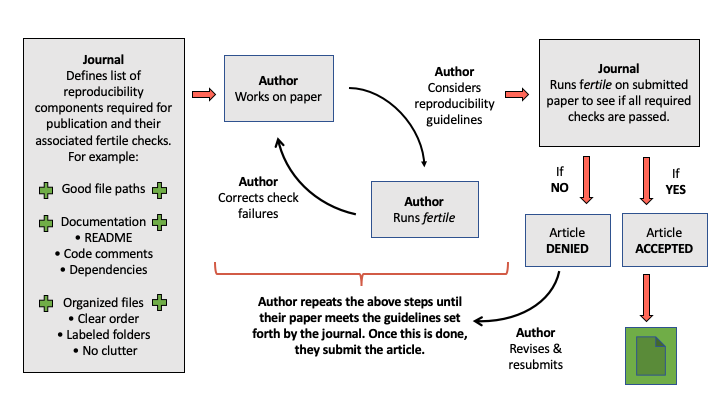
\includegraphics[width=1\linewidth]{figure/journal-process} \caption{Potential 'fertile' Journal Review Process}\label{fig:unnamed-chunk-72}
\end{figure}
\begin{enumerate}
\def\labelenumi{\arabic{enumi}.}
\setcounter{enumi}{1}
\tightlist
\item
  Journal reviewers do not run \texttt{fertile} on each project, but instead require submitting authors to include a \texttt{fertile} summary sheet showing the reproducibility badges awarded to their work.
\end{enumerate}
Some journals may desire a reproducibility summary, but not require details as specific as the exact reasons for failure. These journals could run a simplified approach to reproducibility review. Rather than spend the additional time to run \texttt{fertile} on every submission and review the reasons for check failure, the journals could instead require that authors include a cover sheet---produced by the \texttt{proj\_badges()} function---with their submission.

This cover sheet would show which of the six primary reproducibility components were met and which ones failed, a short summary of specific checks that were not successful, and information about the cover sheet's generation: who generated it, when, and with which files.

Journals could place an acceptance requirement that articles achieve a certain subset of badges---for instance, file paths, randomness, and documentation. Submitting authors would run \texttt{fertile} on their end to see which badges they passed. Once they met the requirements, they could run \texttt{proj\_badges()} to generate an article cover sheet. This cover sheet would then be submitted alongside the article and considered as part of the review process. All that reviewers would need to do to ensure that reproducibility requirements are met would be to look at the cover sheet to see which badges the project achieved and check the cover sheet generation information to ensure that it was truly produced by the project that the author says it was produced by.
\begin{figure}
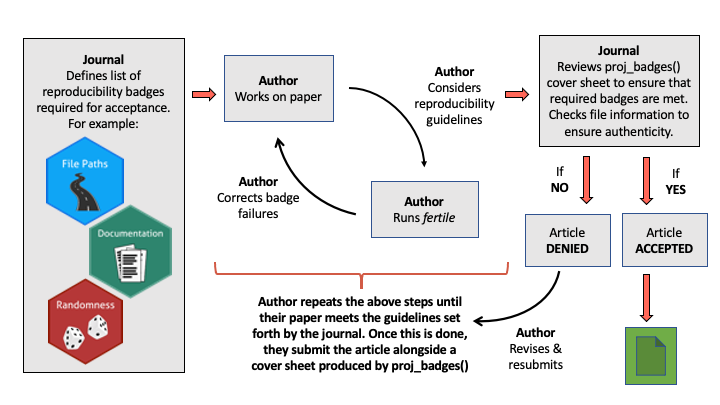
\includegraphics[width=1\linewidth]{figure/journal-process-2} \caption{Another Potential 'fertile' Journal Review Process}\label{fig:unnamed-chunk-73}
\end{figure}
Both of these processes would be much faster than that employed currently at the \emph{American Journal of Political Science}, which goes through a thorough, multi-week-long reproducibility confirmation procedure for all submitted articles. Submitting authors would know exactly which goals they were trying to achieve. They could download \texttt{fertile} on their own, run it on their project, check to see if their goals are met, and take the recommended steps to address failures if not. Then, upon submission, journals would only need to take minimal steps to ensure that those standards were met.

For journals that currently spend little effort on ensuring the reproducibility of submitted articles, \texttt{fertile} could provide significant benefit for minimal cost. Rather than spending money to hire a reproducibility editors, any journal board wanting to improve their publication's reproducibility could instead choose to implement \texttt{fertile}---for free---as part of the review workflow.

Journals that already have designated reproducibility editors, such as \emph{Biostatistics} and the \emph{Journal of the American Statistical Association}, could also benefit from \texttt{fertile} (Biostatistics Staff (2020), JASA Editors (2020)). The integration of \texttt{fertile} could speed up the review process, allowing the editors to review more papers for reproducibility adherence in a shorter time.

Although this would only address a small aspect of reproducibility--that involving data analysis projects written in R--it could save significant time and money for authors and reviewers in that domain.

\hypertarget{for-teaching-reproducibility}{%
\subsection{For Teaching Reproducibility}\label{for-teaching-reproducibility}}

\texttt{fertile} could also be integrated into Statistical and Data Sciences coursework in order to educate students on topics of reproducibility.

Many of the existing programs to teach reproducibility are courses focused on replication studies, where students must take a published paper and replicate the steps within completely. This process, which includes requesting the necessary data and code files from the original author(s) and sometimes even expanding the existing analysis further, often requires that participants have knowledge of data analysis and the scientific research process to be successful. As a result, such courses focused on reproducibility tend to exist only at the graduate level.

Undergraduate students do not have the same level of access to reproducibility education. Some schools prioritize reproducibility education--for instance, courses at Smith College and Duke University integrate reproducibility through the use of RMarkdown (Baumer, Cetinkaya-Rundel, Bray, Loi, \& Horton (2014))--but not all do, and most not at as in-depth of a level as masters courses.

\texttt{fertile} could help change this, allowing for many more colleges and universities to integrate reproducibility into their courses as a primary topic of focus. The barriers to entry for using and benefiting from the package are very low, requiring only that participating students have:
\begin{itemize}
\tightlist
\item
  R and RStudio installed on their computer
\item
  Knowledge of how to install a package from GitHub and load it into their environment
\item
  Knowledge of how to create an R project
\item
  Knowledge of how to run basic functions and input simple file paths
\end{itemize}
Although the process may entail some confusion and troubleshooting at first, even those brand new to \texttt{R} could succeed in overcoming these barriers in only a few days of class. As a result, \texttt{fertile} could provide professors with an opportunity to teach reproducibility concepts in introductory level courses.
\begin{figure}
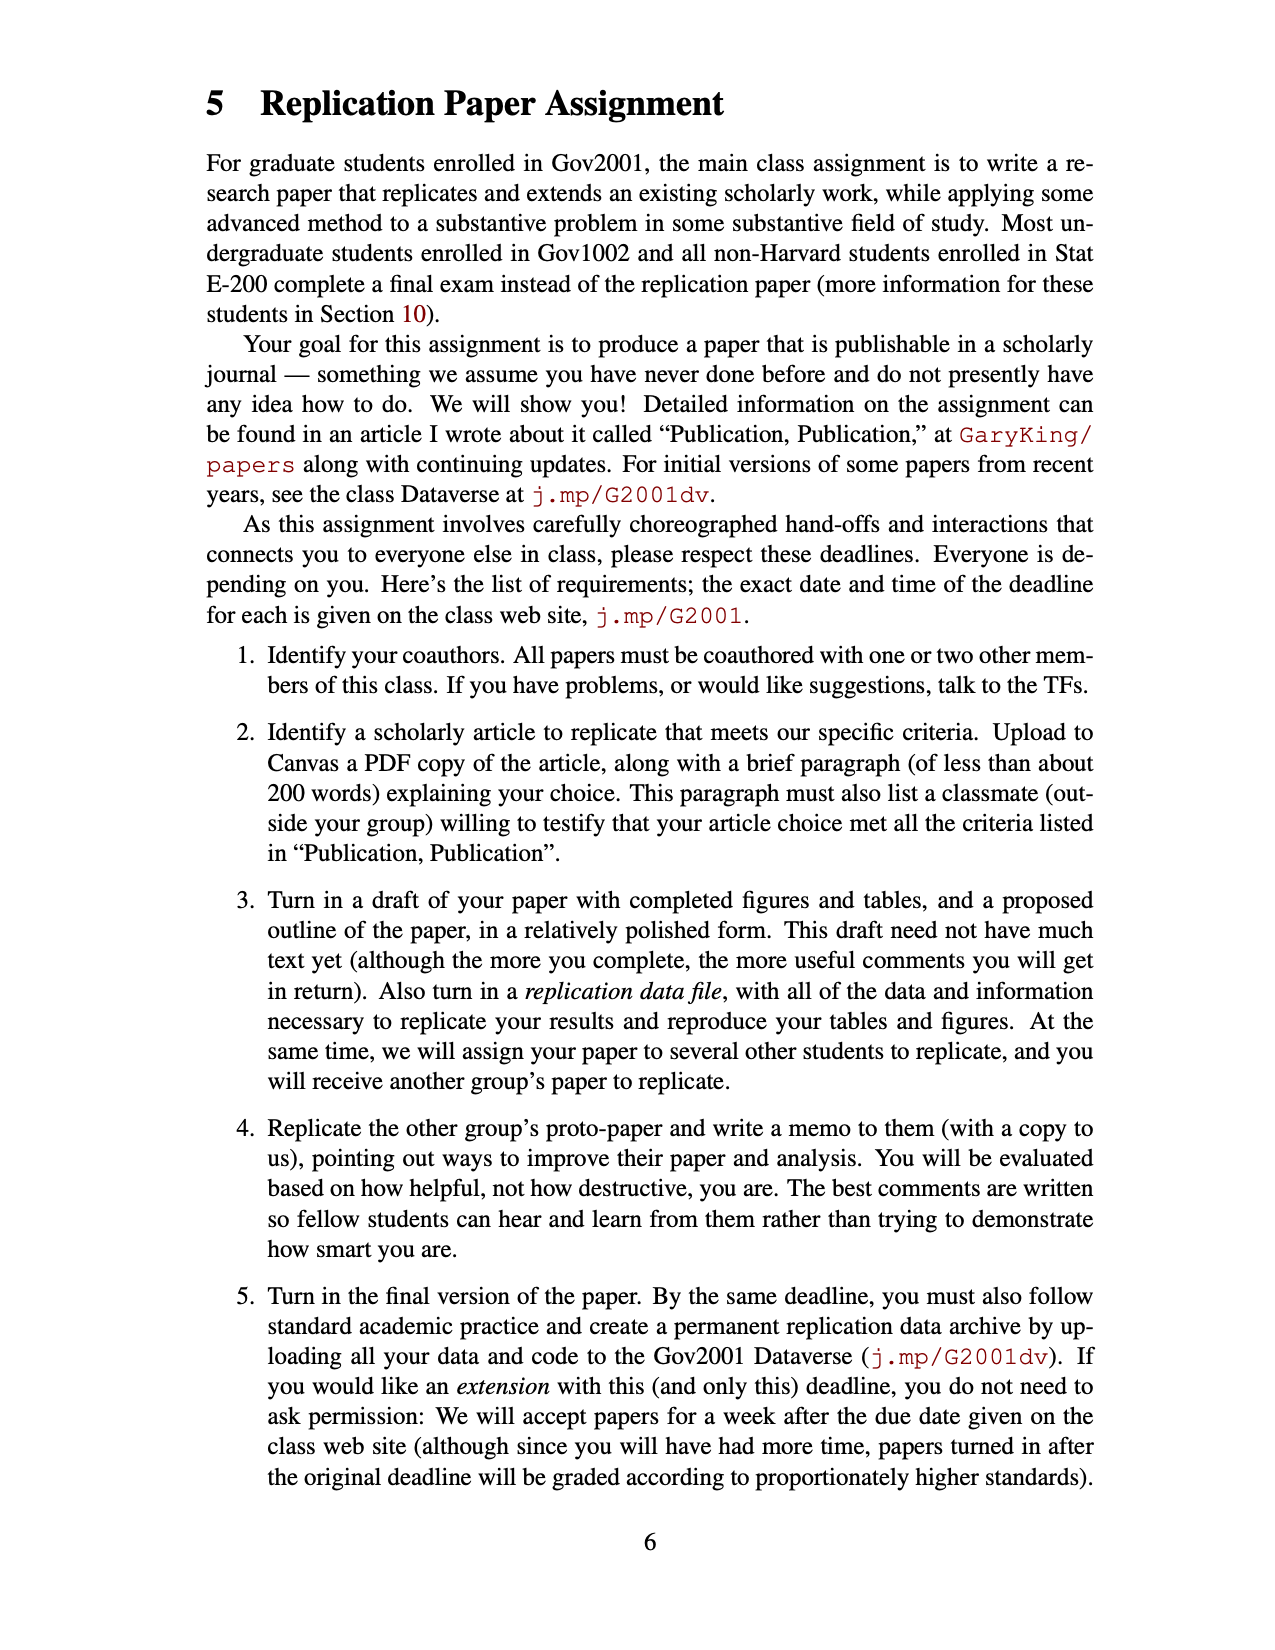
\includegraphics[width=1\linewidth]{figure/gov-2001-replication} \caption{The Replication Assignment From Harvard Professor Gary King's Gov 2001 Graduate Course}\label{fig:unnamed-chunk-74}
\end{figure}
\texttt{fertile} could easily integrate into coursework in a similar way to how RMarkdown was integrated at Smith College and Duke University. While there is not only one way to utilize the software in class, a potential use of \texttt{fertile} could look as follows:

At the beginning of their course, the professor provides their students with a brief introduction to reproducibility, including its importance and a basic description of how it is achieved. Shortly after, they introduce R Projects and the \texttt{fertile} package, explaining that they are tools to help with reproducibility. Then, they institute a requirement for all submitted homework assignments in the course: students must create and submit their work in the R Project format, but prior to submission must run \texttt{fertile} on their project to ensure that it passes reproducibility standards. When reproducibility errors inevitably occur, they can be used as teachable moments: the professor can share the error, explain why it happened, walk through \texttt{fertile}'s response to it, and interactively work with students to illustrate how it can be fixed.

The integration of \texttt{fertile} in this way would be an excellent method to introduce students to reproducibility concepts early on in their data science education, but at a low cost to the professor.

I believe that there are a variety of potential benefits to introducing students to reproducibility sooner, rather than later--in graduate school or through independent research on the topic:
\begin{itemize}
\item
  Teaching reproducibility early on could help give students important research tools and understanding before they conduct any of their own important analysis.
\item
  Practicing before students are believed to be skilled and highly educated in data science could afford them an opportunity to fail and learn without fear of judgment.
\item
  Integrating concepts early through repetitive use and recall helps ingrain them in the minds of students, ensuring that reproducibility begins to come naturally to them (Karpicke \& Roediger (2008)).
\end{itemize}
These students would then be prepared for entering the research world and contributing to data science work in a transparent and reproducible way.

\hypertarget{in-other-areas}{%
\subsection{In Other Areas}\label{in-other-areas}}

\texttt{fertile} can also provide benefits in other domains. Although not an exhaustive list, some of the potential uses of the software are:
\begin{itemize}
\item
  \emph{Private Companies}: Data analysis-focused companies could require their employees to use \texttt{fertile} to check the reproducibility of their projects before presenting them to clients. This would help such companies ensure that clients could trust the results that were being produced.
\item
  \emph{Conferences}: Similar to academic journals, conferences promoting open research could require that papers written in \texttt{R} pass a \texttt{fertile} check as a condition for acceptance. Even if there were an exception given for those using confidential/identifiable data, this would likely increase the overall reproducibility of conference papers significantly.
\item
  \emph{Informal Data Analysis}: A lot of content in the \texttt{R} community is created purely for fun and interest. Outside of work, many \texttt{R} users will create data visualizations or analyses for their own private blogs or their twitter. Sometimes, users will also participate in community events like Tidy Tuesday, a weekly social project where a data set is posted and users are asked to analyze it and create a visualization of their choice. Many people use these informal analyses as an opportunity for learning and discussion, often sharing them on social media to try and get feedback on their work. Ensuring that the work is reproducible would facilitate this process. Users could run their project files through \texttt{fertile} to check that they are reproducible and post a link to download them. This would then allow others to run the code on their own to understand how it works and more easily be able to make suggestions as to how to improve it!
\end{itemize}
\begin{figure}
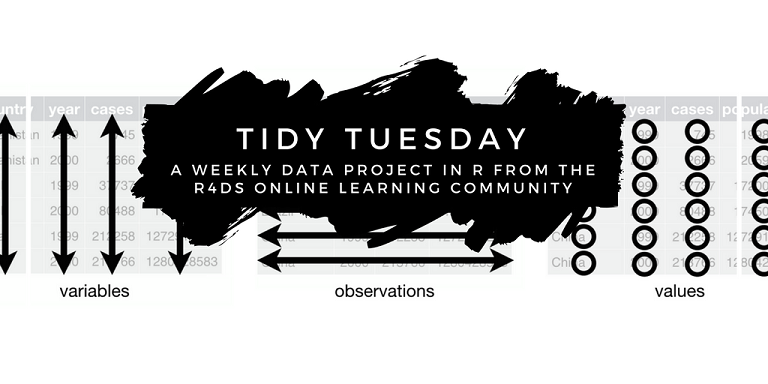
\includegraphics[width=1\linewidth]{figure/tidytuesday} \caption{The Logo For Popular Tidy Tuesday Event}\label{fig:unnamed-chunk-75}
\end{figure}
\texttt{fertile} is versatile in its applicability. It can be used anywhere from informal data analysis projects to academic journal review.

\hypertarget{testing-fertile-in-the-real-world-experimental-design-and-analysis}{%
\section{Testing fertile in the Real World: Experimental Design and Analysis}\label{testing-fertile-in-the-real-world-experimental-design-and-analysis}}

\hypertarget{background}{%
\subsection{Background}\label{background}}

Many of the suggested uses for \texttt{fertile} in the previous section are hypothetical, included for the purpose of demonstrating the potential that the package could have. Without experimentation or testing, though, it is difficult to know just how successful \texttt{fertile} would be when employed for any given purpose.

In order to gain a better understanding of the practical effects of using \texttt{fertile} in a real life scenario, Professor Baumer and I decided to conduct an experiment (approved by Smith College IRB, Protocol \#19-032). We were interested in testing whether the integration of \texttt{fertile} into an introductory data science course might have an effect on students' learning of reproducibility concepts.

After designing our experimental structure, working out technical mechanics, and creating the necessary materials, we chose to use the following two course sections for our study:
\begin{enumerate}
\def\labelenumi{\arabic{enumi}.}
\tightlist
\item
  Introduction to Data Science (SDS 192), Fall 2020 Semester
\item
  Introduction to Data Science (SDS 192), January-Term 2021
\end{enumerate}
There were several motives for selecting these specific courses:
\begin{itemize}
\tightlist
\item
  They were both being taught by Prof.~Baumer, which made it easy to ensure that everything went smoothly by removing the need to interact with a 3rd party.
\item
  They were two different sessions of the same course, with essentially identical material, ensuring that we could combine results from each section of the experiment.
\item
  They involved introductory data science students, one of the groups that were of most interest as we wanted to ensure that \texttt{fertile} could provide benefit to users of all skill levels.
\item
  Though certainly not large sample sizes by any measure, they were still somewhat larger than many other classes in the Statistical and Data Sciences department, providing an opportunity for more data collection.
\end{itemize}
\hypertarget{experimental-design}{%
\subsection{Experimental Design}\label{experimental-design}}

For the experimental structure, we chose to complete a randomized controlled trial (RCT) since RCT designs can be used to conclude causality and are designed in such a way as to limit bias in the results.

Our goal was to determine whether students who had \texttt{fertile} installed and loaded on their RStudio applications would learn more about reproducibility throughout the course than students who did not, or whether there was instead no difference or even a negative effect.

In order to measure this potential effect, we opted to use reproducibility ``tests,'' forms containing multiple choice and select-all-that-apply questions about different aspects of reproducibility that are focused on in \texttt{fertile}.

We used two different testing structures for our two experimental sections--partially due to challenges which led to our first experiment session starting on a slight delay, but also so that we could compare which structure worked more effectively. While the primary goal of the experiment was to determine the effect of \texttt{fertile}, a secondary interest was in the experimental method itself--a new method that we developed, which has implications beyond purely this case.
\begin{itemize}
\item
  Structure \#1 (Used in Fall 2020): Students received a reproducibility test at the end of the semester to test their knowledge after the course. Final scores were compared between students who had \texttt{fertile} installed and loaded and those who did not.
\item
  Structure \#2 (Used in January Term 2021): Students received a reproducibility test both at the beginning of the course \emph{and} at the end of the course in order to test their \emph{change} in knowledge. \emph{Differences in scores} were compared to see if any given group learned more, less, or the same.
\end{itemize}
Although the testing structures were different across the two different sections, the reproducibility tests were identical.

To reduce bias, we opted to use blinding, in which participants were unaware of whether they had received the experimental or control condition--in this case, whether they had \texttt{fertile} installed and loaded while working on course assignments, or whether they didn't.

To achieve the desired blinding, we decided to use some features of R packages which allowed us to give all students in the course the same software, but have it behave differently when loaded, depending on which experimental group the student was a part of.
This technique is described in the step by step experimental structure, explained below:
\begin{enumerate}
\def\labelenumi{\arabic{enumi}.}
\item
  Students were given a form at the start of the semester asking whether they consented to participate in a study on data science education. Additionally, information was collected about the previous number of courses that student had taken in data/computer science fields, which we believed might impact their knowledge of reproducibility. In order to successfully consent, students had to provide a unique computer identifier, collected through the command \texttt{whoami::username()}. This identifier was collected in order to ensure that students could be individually identified and therefore assigned effectively to treatment or control groups.
\item
  To maintain student privacy, the unique identifiers were then transformed into hexadecimal strings via the \texttt{md5()} hashing function. To the students' computers, and us---the researchers---these hashed strings contained the same information as the identifiable usernames, but to those without the original identifier, they appear only as a meaningless string of letters and numbers.
\item
  These hexadecimal strings, which correspond to unique students, were then randomly assigned into equally sized groups, one experimental group that receives the features of \texttt{fertile} and one group that receives a control.
\end{enumerate}
To ensure an adequate control, with the control group students operating day-to-day in an almost identical way to the experimental group, we created a software package for the course which every student in the class would use, regardless of group. The package, titled \texttt{sds192}, contained several templates and data sets that were necessary for use in the course, so all students in the class--regardless of their experimental status--needed to install it.

The \texttt{sds192} package was designed to look the same to both the experimental and control group students, but to function slightly differently for each. The control group would only have access to the templates and data provided with the \texttt{sds192} package, and the experimental group would have all of those things \emph{plus}, they would have \texttt{fertile} silently loaded in the background. This meant that \texttt{fertile}'s proactive features were enabled, and therefore experimental group users would receive warning messages when they used absolute or non-portable paths or attempted to change their working directory. Control group users, who did not have \texttt{fertile} loaded for them, would not receive these messages.

This control/experimental group differentiation works by leveraging an \texttt{.onAttach()} function in the \texttt{sds192} package to scan the \texttt{R} environment of each student \emph{each time the package is loaded}, collect their unique identifier--again, via \texttt{whoami::username()}-- and run it through the same hashing algorithm as before.

\texttt{sds192} came pre-coded with the hashed identifiers of all of the students, grouped by whether they had been assigned to the experimental or the control group, to facilitate the operation of \texttt{.onAttach()}. Each time a student's hashed identifier was collected (every time they loaded the \texttt{sds192} package for class), it was then compared with the provided groups to determine whether the behavior of the package would match the control or experimental group.

The structure of this function can be seen below:
\begin{Shaded}
\begin{Highlighting}[]
\CommentTok{\# .onAttach() from the sds192 package}
\CommentTok{\# Run automatically any time the sds192 package is loaded}

\NormalTok{.onAttach }\OtherTok{\textless{}{-}} \ControlFlowTok{function}\NormalTok{(libname, pkgname) \{}

  \CommentTok{\# The experimental group gets \textasciigrave{}fertile\textasciigrave{} loaded silently}
  \ControlFlowTok{if}\NormalTok{ (}\FunctionTok{is\_experimental}\NormalTok{()) \{}
    \FunctionTok{suppressMessages}\NormalTok{(}\FunctionTok{library}\NormalTok{(fertile))}
\NormalTok{  \}}
\NormalTok{\}}

\NormalTok{is\_experimental }\OtherTok{\textless{}{-}} \ControlFlowTok{function}\NormalTok{(}\AttributeTok{logname =}\NormalTok{ whoami}\SpecialCharTok{::}\FunctionTok{username}\NormalTok{()) \{}
  
  \CommentTok{\# Students are placed into experimental and control}
  \CommentTok{\# groups but remain anonymous}
\NormalTok{  fertile\_group }\OtherTok{\textless{}{-}} \FunctionTok{c}\NormalTok{(}
    \StringTok{"f7b0a9d5117b88cecec122f8ba0e52fb"}\NormalTok{,}
    \StringTok{"4d0295a810fb8491f91f914771572485"}\NormalTok{,}
    \StringTok{"36211a1f19f82ae07aed990b671c9b20"}\NormalTok{,}
    \StringTok{"b5d2b72b4f36f3afdce32a8409dc6ea0"}\NormalTok{,}
    \StringTok{"d498227fd9e6a4c42494bbebc42f6aa8"}\NormalTok{,}
    \CommentTok{\# ... and so on}
\NormalTok{  )}
\NormalTok{  control\_group }\OtherTok{\textless{}{-}} \FunctionTok{c}\NormalTok{(}
    \StringTok{"9aa36583f54766205850428e8f1a4c89"}\NormalTok{, }
    \StringTok{"f03020938b31818063c79d2422755183"}\NormalTok{, }
    \StringTok{"7ec57b1f2bca9ac1e702fb68427b781b"}\NormalTok{, }
    \StringTok{"e5e30623e9d09d29ded851b7fb40cb51"}\NormalTok{, }
    \StringTok{"592572bb9fce168f37117fd0d6e0e5ee"}\NormalTok{,}
    \CommentTok{\# ... and so on}
 
\NormalTok{  )}
  

\NormalTok{  digest}\SpecialCharTok{::}\FunctionTok{digest}\NormalTok{(logname, }\AttributeTok{algo =} \StringTok{"md5"}\NormalTok{) }\SpecialCharTok{\%in\%}\NormalTok{ fertile\_group}
  
\NormalTok{\}}
\end{Highlighting}
\end{Shaded}
\begin{enumerate}
\def\labelenumi{\arabic{enumi}.}
\setcounter{enumi}{3}
\item
  {[}January Term 2021 Only{]} Students then took a reproducibility test prior to fully starting the course, which tested their knowledge before completing the class.
\item
  The students then completed their coursework as normal, regularly using the \texttt{sds192} package for projects and homework assignments.
\item
  {[}Both Fall 2020 and January Term 2021{]} The last step was for students to take a reproducibility test at the end of the course, to measure their knowledge of the subject after having completed the coursework and used the \texttt{sds192} package.
\end{enumerate}
\hypertarget{results}{%
\subsection{Results}\label{results}}

In order to understand the results, it is important to understand the structure of the experimental reproducibility ``test'' and the way in which each student's answers were scored.

The test consisted of two primary sections:
\begin{enumerate}
\def\labelenumi{\arabic{enumi}.}
\item
  A set of six questions on RStudio projects, two of which were select-all-that-apply, and four of which were multiple choice. These questions tested students knowledge of RStudio projects, their understanding of which file paths they could include in code submitted in project format, and their awareness of the dangers of changing working directories while coding.
\item
  A set of three questions about file paths, all of which were select-all-that apply. These questions tested students' knowledge of the difference between absolute and relative paths and their understanding of which paths are reproducible.
\end{enumerate}
For reference, the full list of questions is provided in Appendix B.

For each test submission, every question was scored individually and then scores for each section (projects and paths) were calculated, as well as an overall total score.

The following method was used to compute scores:
\begin{itemize}
\item
  For each question, students would start at a score of zero. Based on their answers, points would then be added, subtracted, or stay constant.
\item
  On select-all-that apply questions, the following scoring rules were used. This meant that students who answered some things correctly, but other things incorrectly, could still receive negative or neutral scores, based on the overall analysis of how correct they were:
  \begin{itemize}
  \tightlist
  \item
    Each correct box that was checked --\textgreater{} +1 Point
  \item
    Each incorrect box that was checked --\textgreater{} -1 Point
  \item
    Each box not checked but should have been --\textgreater{} No change (0)
  \end{itemize}
\item
  On multiple choice questions, the scoring rules were slightly different. This was due to the inclusion of an option for ``I'm not sure,'' which was included as a way to discourage random guessing and ensure that students were answering based on their actual knowledge.
  \begin{itemize}
  \tightlist
  \item
    If the correct answer was selected --\textgreater{} +1 Point
  \item
    If the incorrect answer was selected --\textgreater{} -1 Point
  \item
    If the student expressed uncertainty (``I'm not sure'') --\textgreater{} No change (0)
  \end{itemize}
\end{itemize}
This method meant that individual questions could have negative, positive, or neutral scores, and total scores could vary quite dramatically, from large negative scores (\textless-10) for students who regularly answered incorrectly to large positive scores for those who often answered correctly (\textgreater10).

\hypertarget{fall-2020-results}{%
\subsubsection{Fall 2020 Results}\label{fall-2020-results}}

The data from Fall 2020, after being scored and cleaned up, looked as follows:
\begin{Shaded}
\begin{Highlighting}[]
\FunctionTok{glimpse}\NormalTok{(fall2020)}
\end{Highlighting}
\end{Shaded}
\small
\begin{verbatim}
Rows: 18
Columns: 15
$ User_Hash        <chr> "\"67b8da3952e07ba3f2c5c715c4042220\"", "\"f03020938b~
$ Group            <chr> "Control", "Control", "Fertile", "Fertile", "Fertile"~
$ Previous_Classes <dbl> 0, 0, 2, 1, 2, 1, 6, 0, 1, 1, 1, 2, 1, 1, 5, 1, 3, 1
$ Q1_Points        <dbl> 3, 1, 1, 3, 3, 2, 3, 3, 3, 1, 1, 3, 1, 1, 2, 2, 3, 1
$ Q2_Points        <dbl> 0, -1, 0, -1, -1, 1, -1, 1, -1, 0, -1, -1, 0, -1, 1, ~
$ Q3_Points        <dbl> 0, 1, 0, -1, -1, 0, -1, 1, -1, 0, -1, -1, 0, 1, 1, 0,~
$ Q4_Points        <dbl> 1, 1, 1, 1, 1, 0, 1, -1, 1, 0, 1, -1, 0, 1, 1, -1, 1,~
$ Q5_Points        <dbl> -1, 1, 0, 1, 1, 1, 0, 1, 1, 0, -1, 1, 0, -1, 1, -1, 1~
$ Q6_Points        <dbl> 0, 1, 1, 1, 1, 1, 0, 0, 1, 0, 0, 0, 0, 1, 1, -1, 1, 0
$ Q7_Points        <dbl> 2, 2, 3, 0, -1, 3, 3, 3, -1, 2, 2, 2, 2, 2, 3, 1, 2, 2
$ Q8_Points        <dbl> -1, 2, -2, 2, -2, 2, 2, 2, -2, 2, 1, 1, -1, 1, 2, -1,~
$ Q9_Points        <dbl> 1, 1, 0, 2, 2, 2, 2, 2, 1, -1, 1, -2, 0, 1, 1, 1, 2, 2
$ Projects_Total   <dbl> 3, 4, 3, 4, 4, 5, 2, 5, 4, 1, -1, 1, 1, 2, 7, -2, 4, 2
$ Paths_Total      <dbl> 2, 5, 1, 4, -1, 7, 7, 7, -2, 3, 4, 1, 1, 4, 6, 1, 5, 5
$ Overall_Total    <dbl> 5, 9, 4, 8, 3, 12, 9, 12, 2, 4, 3, 2, 2, 6, 13, -1, 9~
\end{verbatim}
\normalsize

There were 18 students who completed the reproducibility test, split evenly into two groups of 9, and 15 variables per student. Since the Fall 2020 section of the experiment contained only one reproducibility test, each student only has one associated observation in the data.
\begin{enumerate}
\def\labelenumi{\arabic{enumi}.}
\tightlist
\item
  \texttt{User\_Hash}: Hashed identifiers, representing unique students.
\item
  \texttt{Group}: A categorical variable summarizing whether the student was in the experimental (\texttt{fertile}) or control group.
\item
  \texttt{Previous\_Classes}: The number of previous data science / computer science courses the student had taken at the start of the semester.
  4-12. \texttt{Qx\_Points}: The number of points scored on each individual question.
\item
  \texttt{Projects\_Total}: The total number of points scored on the six questions associated with R Projects.
\item
  \texttt{Paths\_Total}: The total number of points scored on the three questions associated with file paths.
\item
  \texttt{Overall\_Total}: The total combined score of all nine questions.
\end{enumerate}
The de-identified data, including all 15 variables of interest, are available with open access at \url{https://github.com/ambertin/thesis}.

The score averages for both groups of students were as follows:
\begin{table}[H]

\caption{\label{tab:unnamed-chunk-80}End of Course Reproducibility Test Averages by Group, Fall 2020}
\centering
\begin{tabular}[t]{lrrr}
\toprule
Group & Projects\_Avg & Paths\_Avg & Overall\_Avg\\
\midrule
Control & 3.33 & 4.22 & 7.56\\
Fertile & 2.11 & 2.44 & 4.56\\
\bottomrule
\end{tabular}
\end{table}
These numbers, combined with the visual below seem to indicate, at least in this small sample, that the \texttt{fertile} group actually performed worse overall than the \texttt{control} group.
\begin{figure}
\centering
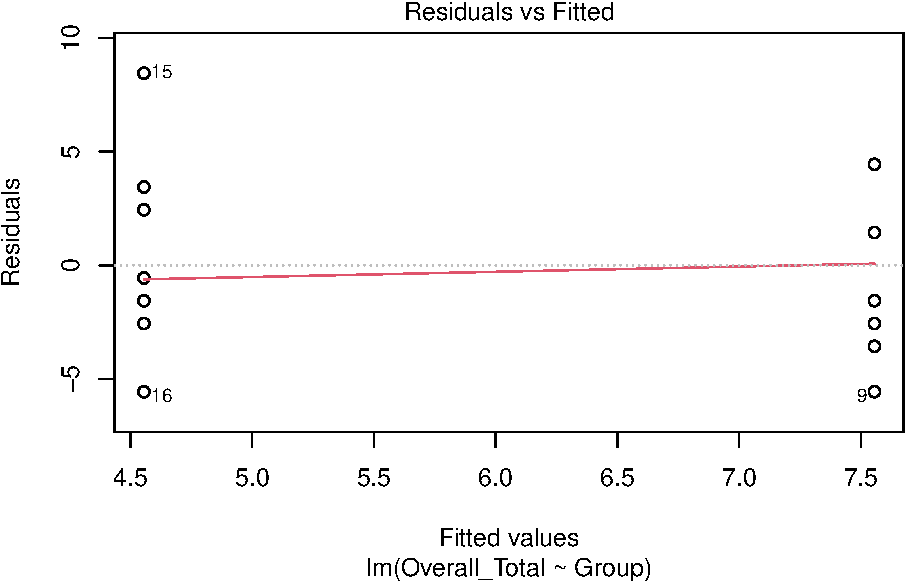
\includegraphics{thesis_files/figure-latex/unnamed-chunk-81-1.pdf}
\caption{\label{fig:unnamed-chunk-81}Bar Chart: End of Course Reproducibility Test Averages by Group, Fall 2020}
\end{figure}
Looking at the overall total score (\texttt{Overall\_Total}), this was true even when controlling for the number of relevant courses taken previously:
\begin{figure}
\centering
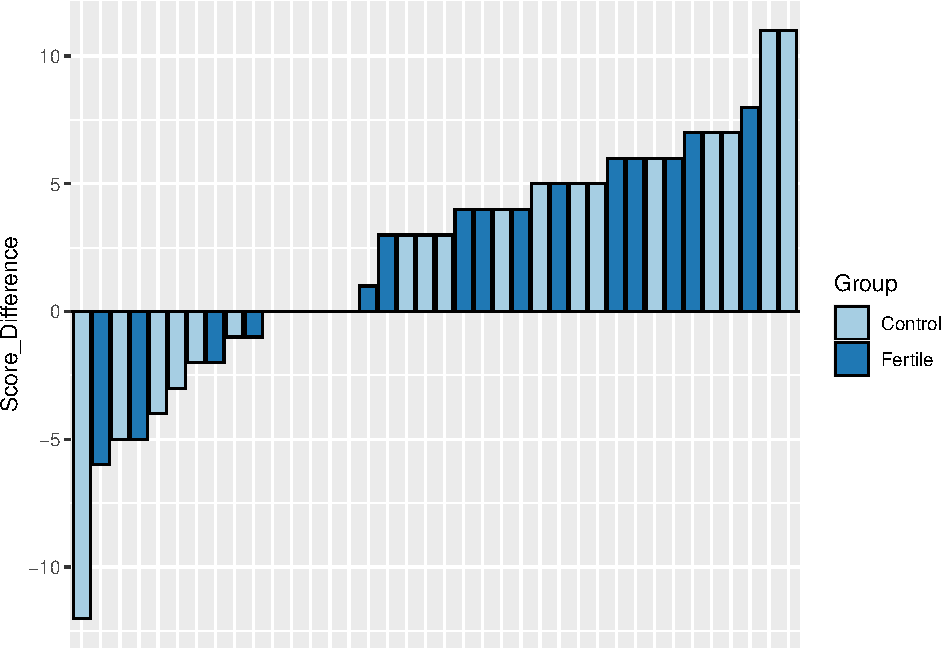
\includegraphics{thesis_files/figure-latex/unnamed-chunk-82-1.pdf}
\caption{\label{fig:unnamed-chunk-82}Scatterplot: Previous Coursework vs Total Reproducibility Test Score, Fall 2020}
\end{figure}
A t-test and analysis of variance (ANOVA) conducted on the simple regression model with independent variable \texttt{Group} and dependent variable \texttt{Overall\_Total} both indicate that, although there is a potential negative trend between the use of \texttt{fertile} and a student's score on the reproducibility test, there is not enough evidence to conclude that this relationship was \emph{not} just the product of chance. The p-values of 0.117 are not below the threshold of 0.05 used to determine statistical significance.
\begin{verbatim}
Call:
lm(formula = Overall_Total ~ Group, data = fall2020)

Residuals:
   Min     1Q Median     3Q    Max 
-5.556 -2.556 -1.056  2.194  8.444 

Coefficients:
             Estimate Std. Error t value Pr(>|t|)    
(Intercept)     7.556      1.281   5.896 2.25e-05 ***
GroupFertile   -3.000      1.812  -1.655    0.117    
---
Signif. codes:  0 '***' 0.001 '**' 0.01 '*' 0.05 '.' 0.1 ' ' 1

Residual standard error: 3.844 on 16 degrees of freedom
Multiple R-squared:  0.1462,    Adjusted R-squared:  0.09288 
F-statistic: 2.741 on 1 and 16 DF,  p-value: 0.1173
\end{verbatim}
\begin{verbatim}
Analysis of Variance Table

Response: Overall_Total
          Df Sum Sq Mean Sq F value Pr(>F)
Group      1  40.50  40.500  2.7406 0.1173
Residuals 16 236.44  14.778               
\end{verbatim}
When fitting a second model, controlling for the number of previous classes, we see a similar result. Although the p-value is smaller (p = 0.08), holding the number of previous classes constant, there is still not enough evidence to suggest that the use of \texttt{fertile} impacts reproducibility test scores.
\begin{Shaded}
\begin{Highlighting}[]
\NormalTok{fall\_model\_mr }\OtherTok{\textless{}{-}} \FunctionTok{lm}\NormalTok{(Overall\_Total }\SpecialCharTok{\textasciitilde{}}\NormalTok{ Group }\SpecialCharTok{+}\NormalTok{ Previous\_Classes, }\AttributeTok{data =}\NormalTok{ fall2020)}
\FunctionTok{summary}\NormalTok{(fall\_model\_mr)}
\end{Highlighting}
\end{Shaded}
\begin{verbatim}
Call:
lm(formula = Overall_Total ~ Group + Previous_Classes, data = fall2020)

Residuals:
   Min     1Q Median     3Q    Max 
-5.191 -2.197 -1.055  2.969  5.803 

Coefficients:
                 Estimate Std. Error t value Pr(>|t|)    
(Intercept)        6.3714     1.4803   4.304 0.000627 ***
GroupFertile      -3.2733     1.7613  -1.858 0.082835 .  
Previous_Classes   0.8198     0.5615   1.460 0.164901    
---
Signif. codes:  0 '***' 0.001 '**' 0.01 '*' 0.05 '.' 0.1 ' ' 1

Residual standard error: 3.715 on 15 degrees of freedom
Multiple R-squared:  0.2525,    Adjusted R-squared:  0.1528 
F-statistic: 2.533 on 2 and 15 DF,  p-value: 0.1128
\end{verbatim}
\hypertarget{january-term-2021-results}{%
\subsubsection{January Term 2021 Results}\label{january-term-2021-results}}

We see a similar story with the data from January Term 2021, though the structure of the data set is different.

The January Term data looks as follows:
\begin{Shaded}
\begin{Highlighting}[]
\FunctionTok{glimpse}\NormalTok{(jterm2021)}
\end{Highlighting}
\end{Shaded}
\small
\begin{verbatim}
Rows: 76
Columns: 17
$ User_Hash        <chr> "\"96eb0673c18b9fa79740686995b1d970\"", "\"980a97cbb1~
$ Student_ID       <dbl> 1, 2, 3, 4, 5, 6, 7, 8, 9, 10, 11, 12, 13, 14, 15, 16~
$ Group            <chr> "Control", "Control", "Fertile", "Fertile", "Fertile"~
$ Previous_Classes <dbl> 1, 1, 2, 1, 1, 4, 3, 0, 0, 1, 1, 4, 3, 4, 2, 4, 4, 0,~
$ Test             <fct> Pre, Pre, Pre, Pre, Pre, Pre, Pre, Pre, Pre, Pre, Pre~
$ Q1_Points        <dbl> 2, 2, 1, 2, 1, 3, 2, 2, 1, 2, 1, 2, 2, 1, 2, 1, 1, 2,~
$ Q2_Points        <dbl> -1, 0, -1, -1, 1, 1, 1, 0, 0, -1, -1, 0, 1, -1, -1, 0~
$ Q3_Points        <dbl> -1, 0, -1, 0, 0, 1, -1, 0, 0, -1, 0, 0, 1, -1, 0, 0, ~
$ Q4_Points        <dbl> 1, 0, 1, 1, 0, 1, 1, 0, 1, 1, -1, 1, 1, 1, 1, 0, 1, 0~
$ Q5_Points        <dbl> 1, 0, -1, 1, 0, 1, -1, 0, 0, -1, 1, 0, 1, 1, 0, 0, 1,~
$ Q6_Points        <dbl> 1, 1, 1, 1, 1, 1, 0, 1, 1, 1, 1, 1, 1, 1, 1, 1, 1, -1~
$ Q7_Points        <dbl> 2, -2, 0, 0, 3, 2, 3, 1, 2, 3, 1, 2, 3, 3, 2, 2, -1, ~
$ Q8_Points        <dbl> 1, -3, -1, -2, 2, 1, 2, 0, 1, 2, 1, 1, 2, 2, 1, 1, -2~
$ Q9_Points        <dbl> 1, 2, 1, 1, 1, 1, -2, 0, -2, 2, -1, -2, 2, 2, -1, 1, ~
$ Projects_Total   <dbl> 3, 3, 0, 4, 3, 8, 2, 3, 3, 1, 1, 4, 7, 2, 3, 2, 6, 1,~
$ Paths_Total      <dbl> 4, -3, 0, -1, 6, 4, 3, 1, 1, 7, 1, 1, 7, 7, 2, 4, -5,~
$ Overall_Total    <dbl> 7, 0, 0, 3, 9, 12, 5, 4, 4, 8, 2, 5, 14, 9, 5, 6, 1, ~
\end{verbatim}
\normalsize

It has many of the same features as the Fall 2020 data, though there are a few differences.
\begin{enumerate}
\def\labelenumi{\arabic{enumi}.}
\item
  This data set contains data on 38 students, rather than 18.
\item
  Each student has two rows of data that correspond to them, rather than just one.
\item
  There are two new variables, \texttt{Student\_ID} and \texttt{Test}. \texttt{Student\_ID} is an index, used to keep track of which rows belong to the same student. This was created as an alternative to \texttt{User\_Hash} as we found that users of Smith College-provided laptop computers would occasionally have non-unique hashed IDs. \texttt{Test} has either the value ``Pre'' or ``Post,'' identifying which test the row corresponds to--the test at the beginning of the course, or the one at the end, respectively.
\end{enumerate}
Just as with the Fall 2020 data, these de-identified data are available publicly at \url{https://github.com/ambertin/thesis}.

When calculating the difference in reproducibility test scores between the end (``Post'') and beginning (``Pre'') of the course, the story looks a little bit less negative than before, but once again there does not appear to be much strong evidence in favor of \texttt{fertile}.

For the questions about file paths, there appears to be no difference in the average score at the beginning and end of the course for either group. For the questions about R Projects, the \texttt{fertile} group had slightly higher average score differences but not by that much (1.92). For the overall total number of points, the score differences were very similar (2.15 for the \texttt{control} group and 2.22 for \texttt{fertile}).
\begin{table}[H]

\caption{\label{tab:unnamed-chunk-89}Average Score Difference Between Beginning/End of Course, January Term 2021}
\centering
\begin{tabular}[t]{lrr}
\toprule
  & Control & Fertile\\
\midrule
Paths & 0.00 & 0.00\\
Projects & 1.20 & 1.89\\
Total & 2.15 & 2.22\\
\bottomrule
\end{tabular}
\end{table}
When considering the distribution of test scores, in addition to just the pure difference, we see a pattern where those students in the \texttt{fertile} group appeared to score worse than the \texttt{control} group, on average. Yet, when considered all together, the \texttt{fertile} group's scores improved slightly more over the time of the course than the \texttt{control} group's.

This evidence appears to strengthen the previous finding--using the Fall 2020 data--that the potential negative relationship between reproducibility test score and use of \texttt{fertile} is likely a product of random chance. In both experimental sections, Fall and January Term, students in the \texttt{fertile} group performed slightly worse than the \texttt{control} group on the reproducibility tests taken at the end of the course. However, the additional evidence from the January Term ``Pre-Test'' appears to indicate that the reason for that lower score might be just that they started from a lower point of knowledge at the beginning, rather than that \texttt{fertile} directly affected their scores.
\begin{figure}
\centering
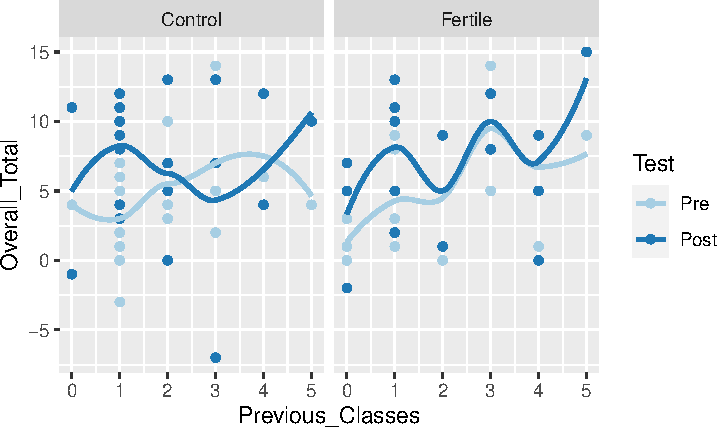
\includegraphics{thesis_files/figure-latex/unnamed-chunk-90-1.pdf}
\caption{\label{fig:unnamed-chunk-90}Boxplot: Pre- and Post-Test Score Distributions by Group, January Term 2021}
\end{figure}
It is also interesting to examine the relationship between the number of previous courses taken by students and their performance on the reproducibility tests.
\begin{figure}
\centering
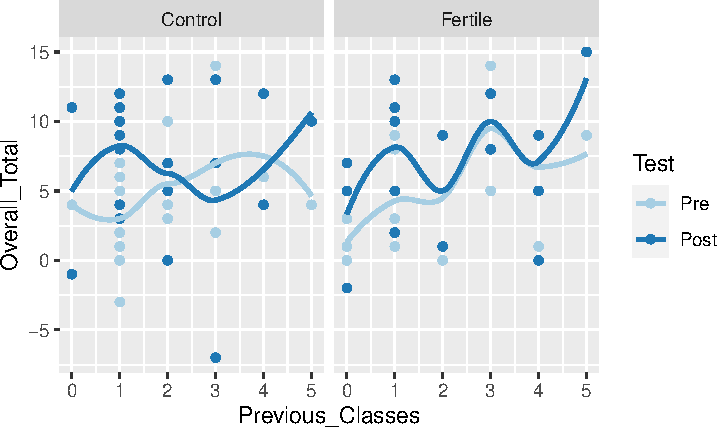
\includegraphics{thesis_files/figure-latex/unnamed-chunk-91-1.pdf}
\caption{\label{fig:unnamed-chunk-91}Scatterplot: Previous Coursework Experience vs Reproducibility Score by Group, January Term 2021}
\end{figure}
Above, we see a graphical representation of the number of previous courses taken by each student and the difference between their overall total score on their Pre- and Post-Tests.

Although it is challenging to make any strong claims with so few data points, one interesting pattern emerges. For the \texttt{control} group, previous experience did not appear to be an indicator of stronger performance or overall learning throughout the course. In some cases, overall performance of students with several previous classes was worse on the Post-Tests than the Pre-Tests. However, with the \texttt{fertile} group, there does appear to be a slight positive relationship between the number of previous classes and the test scores. On average, the \texttt{fertile} group always performed better on their Post-Tests than on their Pre-Tests.

After constructing a simple regression model, predicting overall \texttt{Score\_Difference} based on \texttt{Group} (\texttt{fertile} or \texttt{control}), and running a t-test and analysis of variance, we once again find that there is not enough evidence to argue that \texttt{fertile} provides any benefit in terms of performance on the reproducibility tests. This can be seen with the high p-value of over 0.96, indicating little evidence of a relationship between score differential and group.
\begin{verbatim}
Call:
lm(formula = Score_Difference ~ Group, data = jterm_model_data)

Residuals:
    Min      1Q  Median      3Q     Max 
-14.150  -2.918   0.850   3.546   8.850 

Coefficients:
             Estimate Std. Error t value Pr(>|t|)  
(Intercept)   2.15000    1.10658   1.943   0.0599 .
GroupFertile  0.07222    1.60783   0.045   0.9644  
---
Signif. codes:  0 '***' 0.001 '**' 0.01 '*' 0.05 '.' 0.1 ' ' 1

Residual standard error: 4.949 on 36 degrees of freedom
Multiple R-squared:  5.604e-05, Adjusted R-squared:  -0.02772 
F-statistic: 0.002018 on 1 and 36 DF,  p-value: 0.9644
\end{verbatim}
\begin{verbatim}
Analysis of Variance Table

Response: Score_Difference
          Df Sum Sq Mean Sq F value Pr(>F)
Group      1   0.05  0.0494   0.002 0.9644
Residuals 36 881.66 24.4906               
\end{verbatim}
Adding in a second variable, the number of previous related courses taken by the student, we see the same story. Neither the student's experimental group, nor their number of previous classes have a statistically significant relationship with score difference, holding the other variable constant.
\begin{verbatim}
Call:
lm(formula = Score_Difference ~ Group + Previous_Classes, data = jterm_model_data)

Residuals:
    Min      1Q  Median      3Q     Max 
-13.395  -2.130   1.043   2.996   8.232 

Coefficients:
                 Estimate Std. Error t value Pr(>|t|)  
(Intercept)       3.45431    1.52672   2.263    0.030 *
GroupFertile      0.06459    1.59648   0.040    0.968  
Previous_Classes -0.68648    0.55789  -1.230    0.227  
---
Signif. codes:  0 '***' 0.001 '**' 0.01 '*' 0.05 '.' 0.1 ' ' 1

Residual standard error: 4.914 on 35 degrees of freedom
Multiple R-squared:  0.04152,   Adjusted R-squared:  -0.01325 
F-statistic: 0.7581 on 2 and 35 DF,  p-value: 0.4761
\end{verbatim}
\hypertarget{limitations}{%
\subsection{Limitations}\label{limitations}}

Although the findings of the \texttt{fertile} experiment are interesting, they come with many caveats and should be treated with caution.

For one, the sample sizes of both experimental sections were very small. The first only contained data on 18 students, while the second on only 38. While sample sizes like these may provide some evidence of the existence of experimental relationships, conclusive statements should not be made without additional data.
Even though the SDS 192 courses are some of the largest in the Statistical and Data Sciences department at Smith College, they still did not result in an optimal level of data. Not all students volunteered to participate in the study, several who did failed to complete all of the components necessary for inclusion of their data and---even if everyone had participated---the maximum sample size would have only been limited to the combined size of both course sections: around 100 students.

Second, the fact that the environment for the experiment was an active classroom came with several challenges. Although we wanted students in the experimental group to independently learn from \texttt{fertile} the classroom setting meant that students who had questions about some of the errors that appeared as a result of having \texttt{fertile} loaded would sometimes bring them to Professor Baumer. As the course instructor, he would then be compelled to help them, explaining concepts and clarifying the meaning of any errors, at the expense of any potential effect on the experimental results.

Additionally, students in a classroom have the unfortunate characteristic---in experimental terms---of not being fully independent from one another. Students regularly communicated with each other, asking and answering questions, on a course \texttt{Slack} channel and also worked in groups on many of the class projects. This meant that they could spread knowledge; experiences from the \texttt{fertile} group could be disseminated to the \texttt{control} group and vice versa. Any sort of cross-contamination could be a potential threat to the validity of the experimental results, as independence is a key assumption necessary for linear regression.

Although independence is at risk, many of the other assumptions for linear regression appear to be mostly met.

In the residuals versus fitted values and normal quantile-quantile plots for the Fall 2020 and January Term 2021 data, displayed below in that order, there do not appear to be any trends indicating an egregious lack of adherence to regression conditions.
\begin{figure}
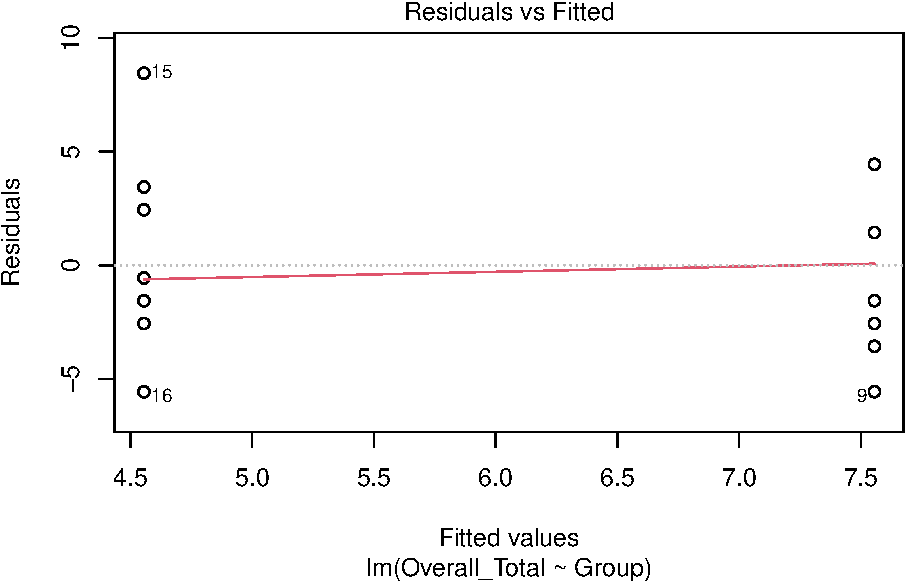
\includegraphics[width=0.5\linewidth]{thesis_files/figure-latex/unnamed-chunk-95-1} 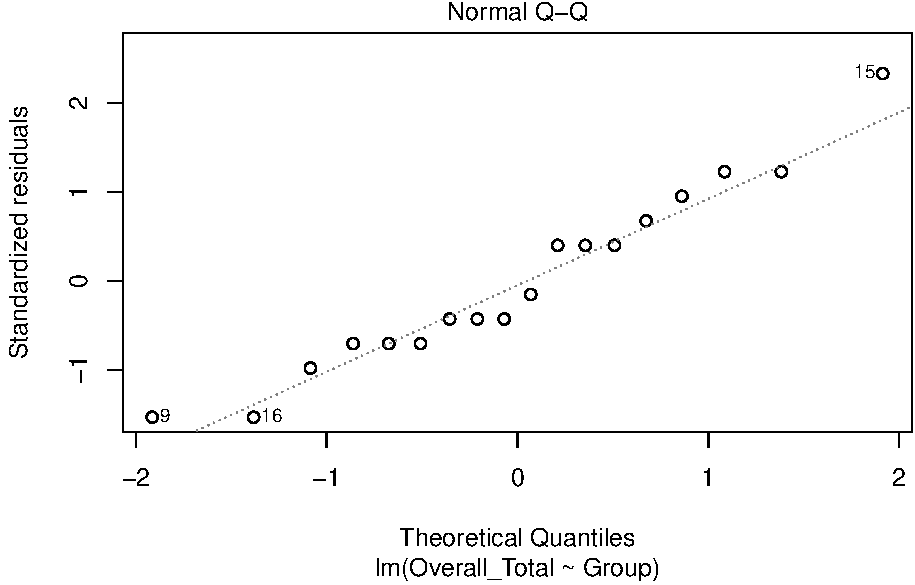
\includegraphics[width=0.5\linewidth]{thesis_files/figure-latex/unnamed-chunk-95-2} 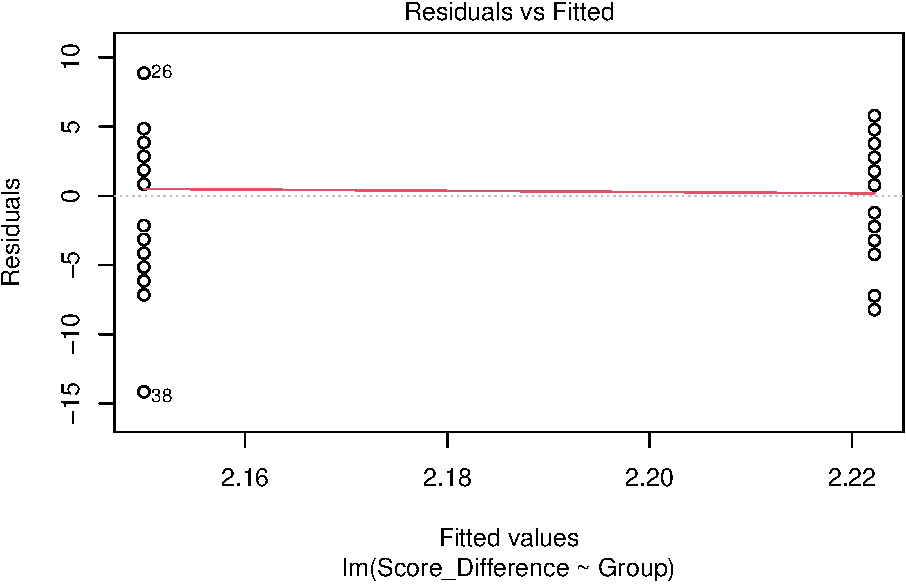
\includegraphics[width=0.5\linewidth]{thesis_files/figure-latex/unnamed-chunk-95-3} 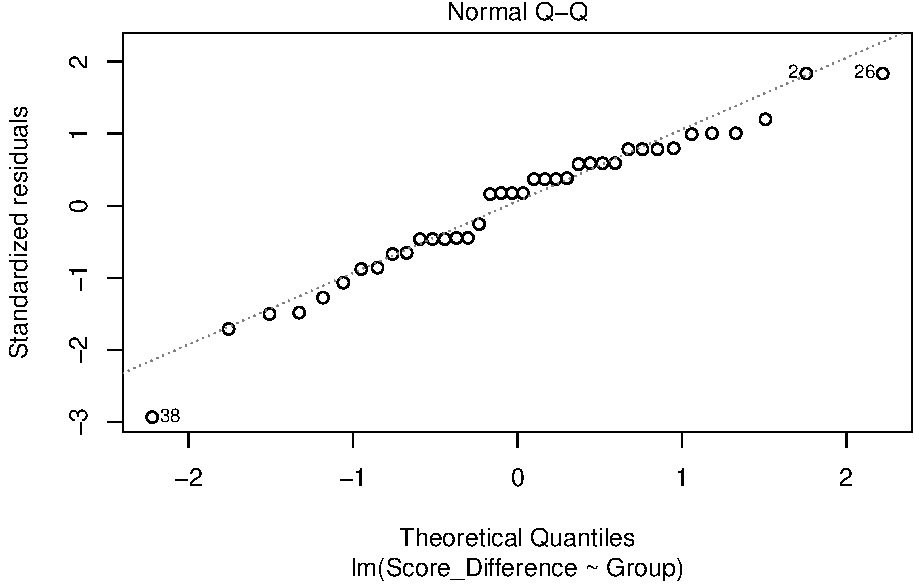
\includegraphics[width=0.5\linewidth]{thesis_files/figure-latex/unnamed-chunk-95-4} \caption{RvF and QQ Plots for Fall 2020 (Top) January Term 2021 (Bottom) Simple Linear Regression Models}\label{fig:unnamed-chunk-95}
\end{figure}
There is the additional limitation that although this experimental structure tests the pure educational power of \texttt{fertile}, it does not accurately represent the ways in which \texttt{fertile} would be used in practice.

Those who use R packages for their own benefit do so with specific intention and knowledge that they are doing so. In practice, unless attempting to do some sort of software testing, no one will use a package that they do not know is loaded.

In order to create an effective experimental environment, however, concessions must be made. If \texttt{fertile} were tested in its natural use state, where students were aware that they were using it, it would introduce the possibility of significant bias in the results. Students in the \texttt{fertile} group, for example, might change their behavior, knowing that their software is designed to improve reproducibility, and pursue extra research into the topic, affecting their test performance. We do not know, from this data, whether \texttt{fertile} has significant benefits in its standard practice. All we can conclude from this study is that in the specific conditions that \texttt{fertile} was used in this course, there was no evidence that the package's interactive reproducibility messaging provides learning benefits when used without students' knowledge.

There is also the fact that the results of this experiment cannot be generalized beyond the Smith College Introduction to Data Science course. In no way is Smith's SDS 192 course representative of the wider undergraduate introductory data science community. Smith classes have a very different student makeup than courses at most other institutions with the distinct feature of being non-male-dominated, so they present a learning environment that is not necessarily comparable. Additionally, the SDS 192 course has its own unique curriculum, not identical to other courses at Smith or at other institutions. Due to the unique course material and teaching methods of SDS 192, students in the class could potentially be more or less primed to process messages about reproducibility compared with students in other courses or at other institutions. In order to gain a better understanding of \texttt{fertile}'s performance in the environments of other colleges and universities, additional studies would be necessary.

Finally, there is the issue of experimental monitoring. After assigning students to experimental and control groups in the \texttt{sds192} \texttt{.onAttach()} function, there is no easy way to monitor that the students in the experimental group had \texttt{fertile} working properly. This would require looking at each student's computer one by one, having them execute potentially reproducibility-breaking commands, and observing the answers, which would be both time consuming and potentially threatening to experimental blindness. Even if \texttt{fertile} were working for an experimental group student at the beginning of the semester, that also does not guarantee that they had it installed for the rest of the semester. That student could have potentially gotten a new computer or changed their unique login name, affecting whether they were correctly recognized as members of the experimental group. There also could have potentially been other bugs on student computers that prevented \texttt{fertile} from loading. Due to these reasons, it is not possible to guarantee that all students in the experimental group had \texttt{fertile} loaded and functioning for the entire semester.

\hypertarget{implications}{%
\subsection{Implications}\label{implications}}

Although the conclusions from this experiment are not particularly demonstrative, the implications of the study extend far beyond just this software.

\hypertarget{implications-for-the-future-of-fertile}{%
\subsubsection{\texorpdfstring{Implications for the Future of \texttt{fertile}}{Implications for the Future of fertile}}\label{implications-for-the-future-of-fertile}}

Through this experiment, we did not discover any significant relationship between students' blind use of \texttt{fertile}'s interactive warning system and their knowledge or learning of reproducibility across the time span of the Introduction to Data Science (SDS 192) course.

Additionally, this experiment does not test \texttt{fertile} in its natural environment---use by an individual who has specifically chosen to use it and studied the documentation in order to understand how it works---or consider the ways in which \texttt{fertile} fills current gaps in software that exist in the \texttt{R} community.

As the project continues to spread and be shared, we hope to find a dedicated community of users who find benefit in its software tools and see an increased shift toward reproducibility in the \texttt{R} community.

\hypertarget{implications-for-the-experimental-design-in-other-applications}{%
\subsubsection{Implications for the Experimental Design in Other Applications}\label{implications-for-the-experimental-design-in-other-applications}}

To the best of our knowledge, the experimental design we developed is the first of its kind---a structure designed to test the difference between two versions of \texttt{R} software without the experimental participants being aware.

Typically, \texttt{R} package testing is primarily anecdotal: a developer will release a software update, request testing and relevant feedback from users, and make edits based on those responses. This method can be effective, but it does not have the same scientific backing behind it as experimental testing does.

If this experimental design gained traction in the \texttt{R} community, it could pave the way for scientific A/B testing of \texttt{R} packages.

A/B testing is an experimental methodology focused on user experience. In an A/B test, designers compare two different versions of a product, randomly assigning participants to groups to determine which version they will receive. Using statistical hypothesis testing, the researchers attempt to identify which software version was most successful.
\begin{figure}
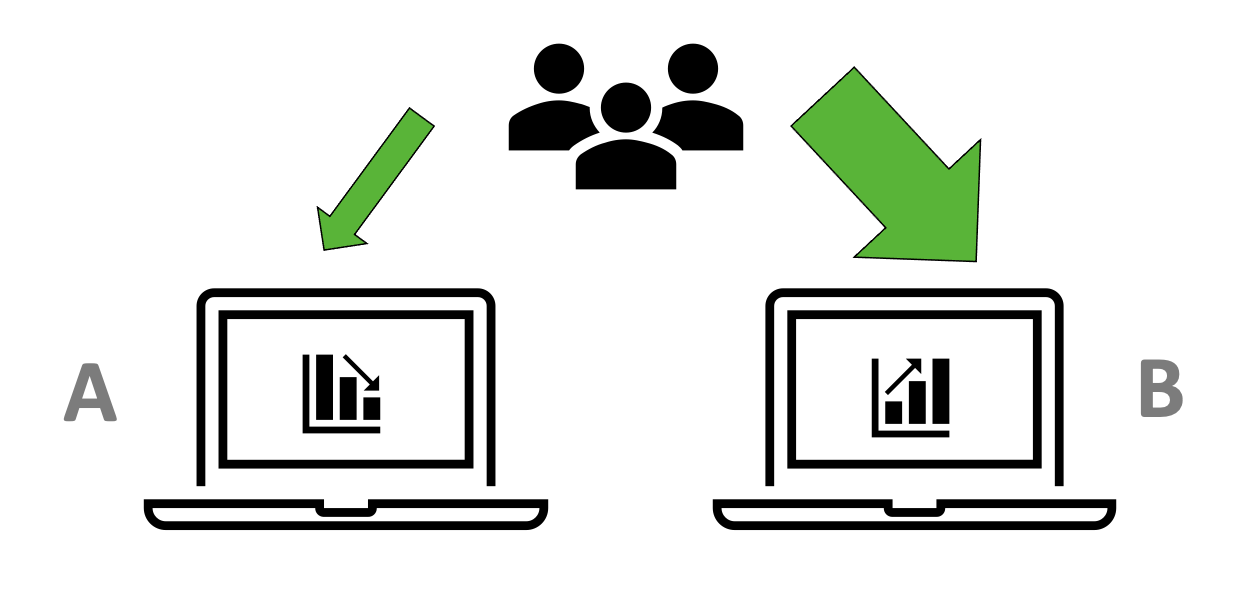
\includegraphics[width=1\linewidth]{figure/a-b_testing} \caption{Scientific A/B Testing}\label{fig:unnamed-chunk-96}
\end{figure}
One of the most popular applications of this form of testing is in marketing. Product sellers, in an attempt to drive traffic to their website and maximize profits, will test several different methods of advertising or web design to see which one results in the most clicks and/or purchase.

Though popular in the marketing industry, A/B testing has the potential to have a positive impact in any software-related domain, including \texttt{R} package development.

This will be particularly useful for those \texttt{R} developers looking to build a deeper scientific understanding of how to code more effectively, and may pave the way for more research-based improvements to software written in the \texttt{R} language.

\hypertarget{conclusion}{%
\chapter*{Conclusion}\label{conclusion}}
\addcontentsline{toc}{chapter}{Conclusion}

In the field of data science, research is considered fully \emph{reproducible} when the requisite code and data files produce identical results when run by another analyst. Though there is no clear consensus on the exact standards necessary to achieve reproducibility, we identify several components of importance:
\begin{enumerate}
\def\labelenumi{\arabic{enumi}.}
\item
  The basic project components are made accessible to the public.
\item
  The file structure of project is well-organized.
\item
  The project is documented well.
\item
  File paths used in code are not system- or user-dependent.
\item
  Randomness is controlled.
\item
  Code is readable and consistently styled.
\end{enumerate}
Reproducibility is vital to the scientific community, helping ensure the accuracy of the findings of studies and data analyses and simplifying the process of collaboration and knowledge sharing. When all of the files necessary for a study to be run are published simultaneously, it makes it much easier for others to understand the methods and ideas that were used and apply them to other work in similar areas, promoting the process of scientific advancement.

However, even though it has many benefits in the scientific community, reproducibility is currently facing a crisis. Many researchers across all scientific fields have been unable to reproduce each other's results, and some have been unable to reproduce even their own. In some fields, more than half of published articles have failed attempts at reproducibility.

Researchers across the sciences have recognized this problem and taken steps to address it. Data-intensive academic journals have put in place reproducibility guidelines requiring that submitted articles meet at least some of the standards listed above. Software developers have built tools to help data analysts make their projects more reproducible. These include a small library of \texttt{R} packages, which provide benefits to users of the popular statistical language \texttt{R}, as well as several continuous integration tools, which are much more broad in their application. Educators have also taken action on reproducibility, introducing courses and workshops focused on the topic at their universities. However, many of these solutions are sub-optimal, facing challenges with inaccessibility, steep learning curves, limited functionality, and/or lack of coding language-specific features.

\texttt{fertile} attempts to fill this gap by being:
\begin{enumerate}
\def\labelenumi{\arabic{enumi})}
\item
  Simple, with a small library of functions/tools that are straightforward to use.
\item
  Accessible to a variety of users, with a relatively small learning curve.
\item
  Able to address a wide variety of aspects of reproducibility, rather than just one or two key issues.
\item
  Language specific, possessing features that address some of the reproducibility challenges associated with \texttt{R}.
\item
  Customizable, allowing users to choose for themselves which aspects of reproducibility they want to focus on.
\item
  Educational, teaching those that use it about why their projects are not reproducible and how to correct that in the future.
\end{enumerate}
Due to its many advantages compared with traditional reproducibility solutions, \texttt{fertile} has the potential to provide benefits in a variety of domains, including in the areas of journal review and education, where other solutions have not quite met the mark.

Integration of \texttt{fertile} into the journal review process---through requirements for passing \texttt{fertile} checks or the inclusion of a \texttt{proj\_badges()} report with a manuscript submission---would greatly reduce the barriers to reproducibility review, speeding up the review process and making it much easier to ensure that published articles are truly reproducible.

In the classroom, \texttt{fertile} could be used to extend reproducibility education to undergraduate students---even those at the introductory level, introducing students to reproducibility much earlier in their data science careers than would likely happen otherwise and increasing the chance that they prioritize reproducibility in their future work.

\texttt{fertile} could also assist the general world of data science, through inclusion of popular events like Tidy Tuesday or integration into workplace environments, among other possibilities.

To test \texttt{fertile\textquotesingle{}s} effectiveness in the classroom, we designed a randomized experiment on an introductory data science course to compare reproducibility learning between students who received \texttt{fertile} on their computer and those who didn't. Although no indication of a relationship between \texttt{fertile} use and knowledge improvement was found in this study---with the caveat that the study format, with blinding, did not fit the intended use of \texttt{fertile} in the real world---the experiment design itself has the potential to open up new avenues of code and package testing in the \texttt{R} community.

\texttt{R} programmers working in a variety of domains could use the experimental structure to employ A/B testing of their software, a type of scientifically-backed testing that has previously not been used---at least to a notable degree---to test \texttt{R} code. This method of testing could pave the way for developers to scientifically measure which coding practices are most effective, efficient, and user-friendly.

Although it is difficult to predict the future of \texttt{fertile}, my hope is for this project is for it to help bring the \texttt{R} community, even if just a few users, toward improved reproducibility and to improve knowledge around the issue within the community. Anything beyond that---journal integration of \texttt{fertile} features, deployment of \texttt{fertile}'s A/B testing design, integration into the workflow by RStudio employees, or the like---would just be the cherry on top.

\hypertarget{a-note-on-limitations}{%
\subsubsection{A Note on Limitations}\label{a-note-on-limitations}}

Although this work focuses primarily on the advantages of \texttt{fertile}, it is important to recognize that \texttt{fertile} is not a be-all, end-all solution to reproducibility. \texttt{fertile} has its own set of limitations, including the following:
\begin{itemize}
\item
  Its work with dependency-management is far less advanced than some other software. Other packages like \texttt{packrat}, for example, go even further, allowing the user to build files containing exact copies of their dependency environment, and add/remove packages as desired.
\item
  \texttt{fertile} has only been under development for a handful of years, much of which was part time by only one or two people as a side project. There are certainly features that would be helpful to be included in the package that have not been, simply because there were only so many things that could be reasonably achieved in the time the package was being written.
\item
  \texttt{fertile} has around 30 software dependencies. This makes it highly susceptible to functionality-breaking changes if some of the functions \texttt{fertile} is dependent on are updated in a way that affects their operation. Unfortunately, this is one of the many trade-offs with \texttt{fertile}: in order to have a library of functions which address all different aspects of reproducibility, a variety of tools are needed, necessitating the use of many imports. This has been a challenge at several points in \texttt{fertile}'s history, requiring the rewriting of functions to address new bugs due to dependency updates. Though not as significant an issue during more recent months, it is likely that more problematic dependency updates will be released in the future.
\item
  As described in Chapter 2, \texttt{fertile} could also be considered a sort of malware, executing operations without the user's knowledge and creating hidden files on their computer. This could be undesirable to some users.
\end{itemize}
For the last two reasons, \texttt{fertile} will likely never be available on CRAN, the official \texttt{R} package hosting site. Its malware-like behavior and high number of dependencies make the package potentially unstable and intrusive, features which are undesirable for packages. This makes \texttt{fertile} slightly less accessible to users who are unfamiliar with the process of installing packages from GitHub or that do not like doing so.

This thesis itself, too, has some limitations. It does not discuss every potential alternative to \texttt{fertile}, many of which have advantages over \texttt{fertile} that should be recognized. It also does not go into detail about every choice made during package development, which could leave out information of interest. Additionally, much of the work in Chapter 3, on potential applications is purely theoretical---there is no evidence of how \texttt{fertile} might actually work in a journal environment or in a classroom under non-experimental conditions. Claims about likely effectiveness are purely based on functionality, and would require much more testing and wide-spread deployment to be backed-up.

Even with all of these limitations, I believe that \texttt{fertile} has a lot of power to do good in the field of reproducibility. If it manages to help even just a few individuals by improving the reproducibility of their work, that is a success.

\appendix

\hypertarget{a-summary-of-relevant-links}{%
\chapter{A Summary of Relevant Links}\label{a-summary-of-relevant-links}}

Several links relevant to \texttt{fertile} were shared throughout the text. To make them easier to find and review, they are all provided together below.
\begin{enumerate}
\def\labelenumi{\arabic{enumi}.}
\item
  GitHub repository for \texttt{fertile}: \url{https://github.com/baumer-lab/fertile}
\item
  My GitHub fork of \texttt{fertile}, where you can track my changes and code contributions more easily: \url{https://github.com/ambertin/fertile}
\item
  GitHub repository for this thesis, which contains the sample project \texttt{project\_miceps}, all of the non-R-generated figures that were included, as well as the de-identified data from the experiment: \url{https://github.com/ambertin/thesis}
\item
  DOI for the paper about \texttt{fertile} which was published in \texttt{Stat}: \url{http://dx.doi.org/10.1002/sta4.332}
\end{enumerate}
\hypertarget{full-overview-of-the-experimental-reproducibility-test}{%
\chapter{Full Overview of the Experimental Reproducibility Test}\label{full-overview-of-the-experimental-reproducibility-test}}

Chapter 3 discusses an experiment that Professor Baumer and myself conducted at Smith College to test \texttt{fertile} in a classroom environment.

In order to measure the package's effectiveness, we constructed a test that could capture information about students' knowledge of reproducibility. The full list of questions on that test, alongside with a step-by-step example of the scoring process, is provided here:

\hypertarget{full-reproducibility-test}{%
\section{Full Reproducibility Test}\label{full-reproducibility-test}}

\hypertarget{test-introduction}{%
\subsubsection{Test Introduction}\label{test-introduction}}


\includegraphics[width=0.8\linewidth]{figure/appendix/test-intro}

\hypertarget{question-1-projects}{%
\subsubsection{Question 1 (Projects)}\label{question-1-projects}}

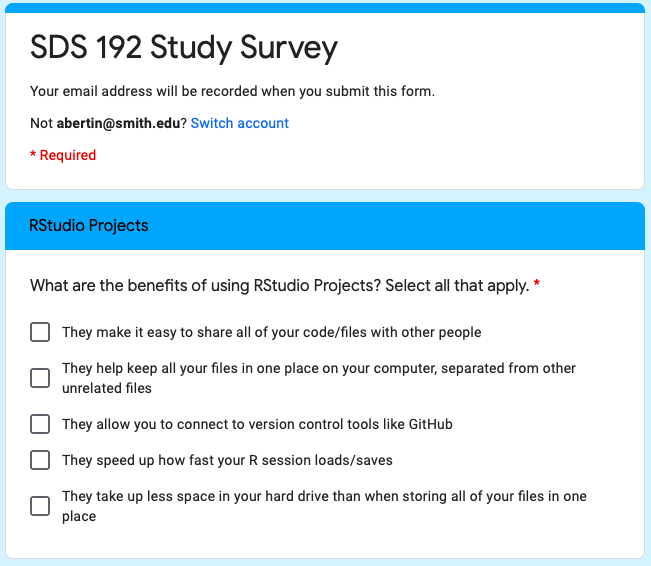
\includegraphics[width=0.8\linewidth]{figure/appendix/test-1}

\textbf{Correct Answers:} 1) They make it easy to share all of your code/files with other people, 2) They help keep all your files in one place on your computer, separated from other unrelated files, 3) They allow you to connect to version controls like GitHub.

\hypertarget{question-2-projects}{%
\subsubsection{Question 2 (Projects)}\label{question-2-projects}}

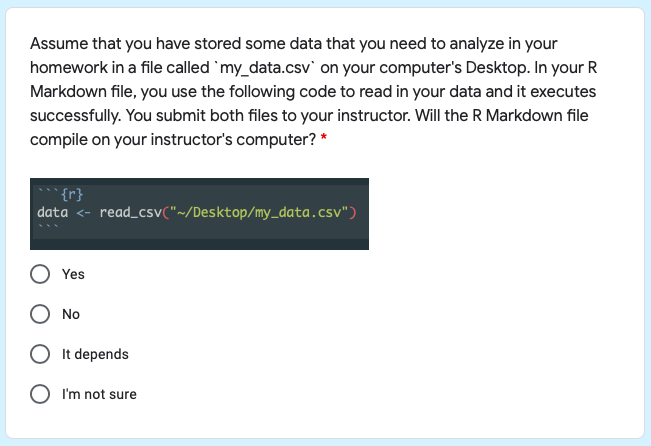
\includegraphics[width=0.8\linewidth]{figure/appendix/test-2}

\textbf{Correct Answer:} ``It depends''

\hypertarget{question-3-projects}{%
\subsubsection{Question 3 (Projects)}\label{question-3-projects}}

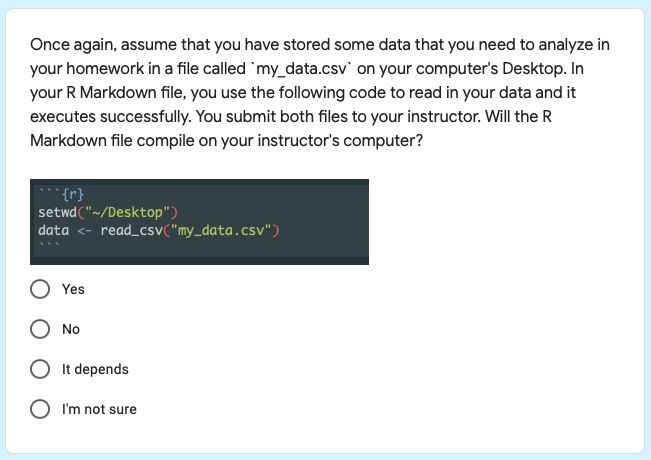
\includegraphics[width=0.8\linewidth]{figure/appendix/test-3}

\textbf{Correct Answer:} ``It depends''

\hypertarget{question-4-projects}{%
\subsubsection{Question 4 (Projects)}\label{question-4-projects}}

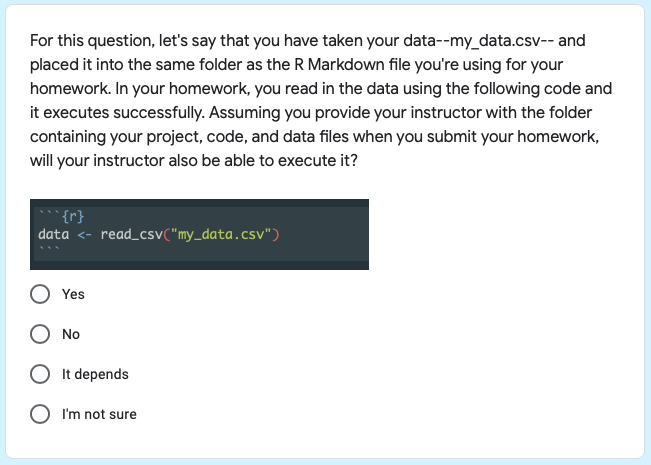
\includegraphics[width=0.8\linewidth]{figure/appendix/test-4}

\textbf{Correct Answer:} ``Yes''

\hypertarget{question-5-projects}{%
\subsubsection{Question 5 (Projects)}\label{question-5-projects}}

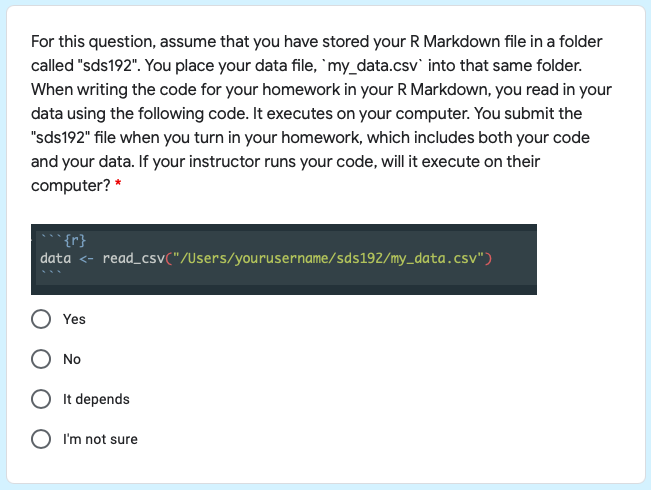
\includegraphics[width=0.8\linewidth]{figure/appendix/test-5}

\textbf{Correct Answer:} ``No''

\hypertarget{question-6-projects}{%
\subsubsection{Question 6 (Projects)}\label{question-6-projects}}

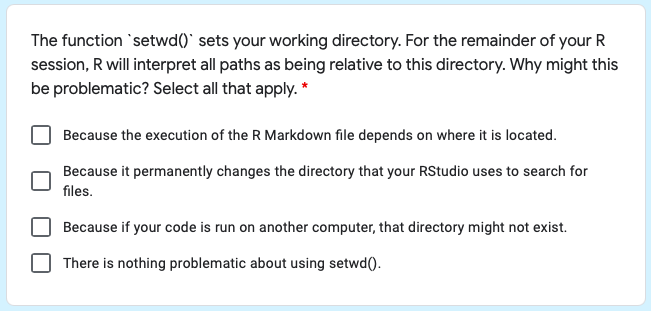
\includegraphics[width=0.8\linewidth]{figure/appendix/test-6}

\textbf{Correct Answers:} 3) Because if your code is run on another computer, that directory might not exist. \textbf{Note}: \emph{1) Because the execution of the R Markdown file depends on where it is located} is sort of ambiguous. Because of this, in scoring, it was considered to be a no change (0) answer if it was selected. Students would not gain or lose points from choosing that answer.

\hypertarget{question-7-paths}{%
\subsubsection{Question 7 (Paths)}\label{question-7-paths}}

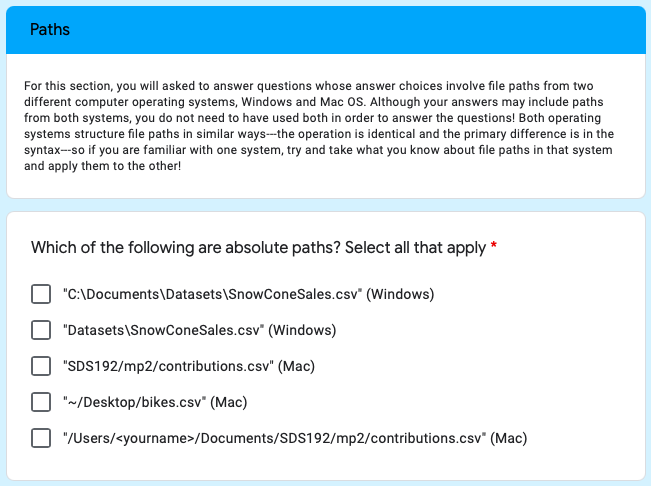
\includegraphics[width=0.8\linewidth]{figure/appendix/test-7}

\textbf{Correct Answers:} 1) \texttt{"C:\textbackslash{}Documents\textbackslash{}Datasets\textbackslash{}SnowConeSales.csv"} ~(Windows), 4) \texttt{"\textasciitilde{}/Desktop/bikes.csv"} (Mac), 5) \texttt{"/Users/\textless{}yourname\textgreater{}} ~
\texttt{/Documents/SDS192/mp2/contributions.csv"} (Mac).

\hypertarget{question-8-paths}{%
\subsubsection{Question 8 (Paths)}\label{question-8-paths}}

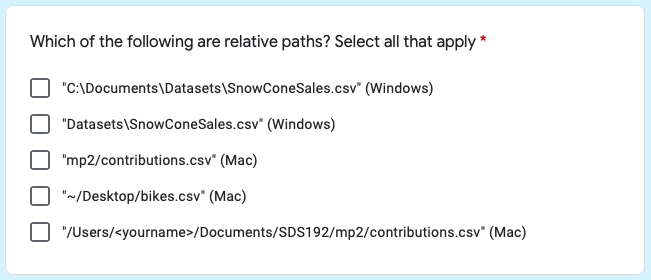
\includegraphics[width=0.8\linewidth]{figure/appendix/test-8}

\textbf{Correct Answers:} 2) \texttt{"Datasets\textbackslash{}SnowConeSales.csv"} (Windows), ~
3) \texttt{"mp2/contributions.csv"} (Mac).

\hypertarget{question-9-paths}{%
\subsubsection{Question 9 (Paths)}\label{question-9-paths}}

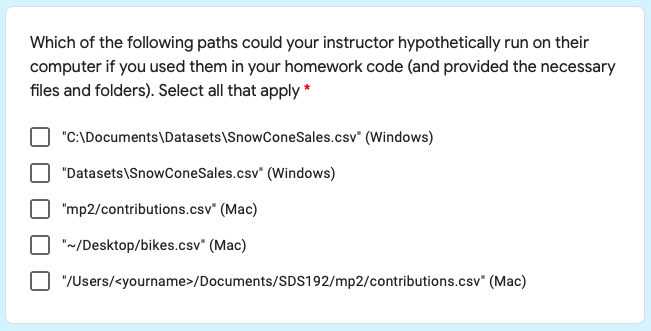
\includegraphics[width=0.8\linewidth]{figure/appendix/test-9}

\textbf{Correct Answers:} 2) \texttt{"Datasets\textbackslash{}SnowConeSales.csv"} (Windows), 3) \texttt{"mp2/contributions.csv"} (Mac). \textbf{Note}: 1) and 4) might also be considered plausible, as they could theoretically work under some conditions, though after some discussion, Professor Baumer and I decided that they would be marked incorrect due to the wording of the question, which specifies that you provide the files and folders.

\hypertarget{sample-scoring-example}{%
\section{Sample Scoring Example}\label{sample-scoring-example}}

Below, we will consider a student's sample answers to this reproducibility test and how they will be scored. As discussed in Chapter 3, the following scoring method was used:
\begin{itemize}
\item
  For each question, students would start at a score of zero. Based on their answers, points would then be added, subtracted, or stay constant.
\item
  On select-all-that apply questions, the following scoring rules were used. This meant that students who answered some things correctly, but other things incorrectly, could still receive negative or neutral scores, based on the overall analysis of how correct they were:
  \begin{itemize}
  \tightlist
  \item
    Each correct box that was checked --\textgreater{} +1 Point
  \item
    Each incorrect box that was checked --\textgreater{} -1 Point
  \item
    Each box not checked but should have been --\textgreater{} No change (0)
  \end{itemize}
\item
  On multiple choice questions, the scoring rules were slightly different. This was due to the inclusion of an option for ``I'm not sure,'' which was included as a way to discourage random guessing and ensure that students were answering based on their actual knowledge.
  \begin{itemize}
  \tightlist
  \item
    If the correct answer was selected --\textgreater{} +1 Point
  \item
    If the incorrect answer was selected --\textgreater{} -1 Point
  \item
    If the student expressed uncertainty (``I'm not sure'') --\textgreater{} No change (0)
  \end{itemize}
\end{itemize}
Prior to scoring question 1, the total score of the student is set at 0, as is their projects questions score and paths questions score.

\hypertarget{question-1-projects-1}{%
\subsubsection{Question 1 (Projects)}\label{question-1-projects-1}}

A student has selected all of the following options:
\begin{itemize}
\tightlist
\item
  They make it easy to share all of your code/files with other people (CORRECT)
\item
  They help keep all your files in one place on your computer, separated from other unrelated files (CORRECT)
\item
  They allow you to connect to version control tools like GitHub (CORRECT)
\item
  They speed up how fast your R session loads/saves (NOT CORRECT)
\item
  They take up less space in your hard drive than when storing all of your files in one place (NOT CORRECT)
\end{itemize}
This student will receive {[}+1{]} for each of the three correct answers, and {[}-1{]} for each of the two incorrect ones, for a total of \textbf{{[}+1{]}}, for a new total score of 1. Since this question was about R projects, the student will also increase their \texttt{Projects\ Score} from 0 to 1.

\emph{Question Score}: 1 \emph{Projects Score}: 1 \emph{Total Score}: 1

\hypertarget{question-2-projects-1}{%
\subsubsection{Question 2 (Projects)}\label{question-2-projects-1}}

The student has selected the following answer:
\begin{itemize}
\tightlist
\item
  Yes (NOT CORRECT) --- the correct answer is ``It Depends''
\end{itemize}
The student will receive {[}-1{]} for this answer, since it is incorrect. This will be added to their previous projects score and total score, resulting in the following updated scores:

\emph{Question Score}: -1 \emph{Projects Score}: 0 \emph{Total Score}: 0

\hypertarget{question-3-projects-1}{%
\subsubsection{Question 3 (Projects)}\label{question-3-projects-1}}

The student has selected the following answer:
\begin{itemize}
\tightlist
\item
  Yes (NOT CORRECT) --- the correct answer is ``It Depends''
\end{itemize}
The student will receive {[}-1{]} for this answer, since it is incorrect. This will be added to their previous projects score and total score, resulting in the following updated scores:

\emph{Question Score}: -1 \emph{Projects Score}: -1 \emph{Total Score}: -1

\hypertarget{question-4-projects-1}{%
\subsubsection{Question 4 (Projects)}\label{question-4-projects-1}}

The student has selected the following answer:
\begin{itemize}
\tightlist
\item
  Yes (CORRECT)
\end{itemize}
The student will receive {[}+1{]} for this answer, since it is correct. This will be added to their previous projects score and total score, resulting in the following updated scores:

\emph{Question Score}: 1 \emph{Projects Score}: 0 \emph{Total Score}: 0

\hypertarget{question-5-projects-1}{%
\subsubsection{Question 5 (Projects)}\label{question-5-projects-1}}

The student has selected the following answer:
\begin{itemize}
\tightlist
\item
  No (CORRECT)
\end{itemize}
The student will receive {[}+1{]} for this answer, since it is correct. This will be added to their previous projects score and total score, resulting in the following updated scores:

\emph{Question Score}: 1 \emph{Projects Score}: 1 \emph{Total Score}: 1

\hypertarget{question-6-projects-1}{%
\subsubsection{Question 6 (Projects)}\label{question-6-projects-1}}

The student has clicked one of the boxes:
\begin{itemize}
\tightlist
\item
  Because if your code is run on another computer, that directory might not exist (CORRECT)
\end{itemize}
The student will receive {[}+1{]} for this answer, since the box they chose was correct. Their choice not to select any other boxes will not affect their score. This will be added to their previous projects score and total score, resulting in the following updated scores:

\emph{Question Score}: 1 \emph{Projects Score}: 2 \emph{Total Score}: 2

At the end of the section on projects, the student has gained a projects score of 2 and is at a total score of 2 as well.

\hypertarget{question-7-paths-1}{%
\subsubsection{Question 7 (Paths)}\label{question-7-paths-1}}

The student has clicked two of the boxes:
\begin{itemize}
\tightlist
\item
  \texttt{"C:\textbackslash{}Documents\textbackslash{}Datasets\textbackslash{}SnowConeSales.csv"} (Windows) (CORRECT)
\item
  \texttt{"\textasciitilde{}/Desktop/bikes.csv"} (Mac) (CORRECT)
\end{itemize}
The student will receive {[}+2{]} for this answer, since both of the boxes they chose was correct. Their choice not to select any other boxes will not affect their score. This will be added to their their paths score (which started at zero) and total score, resulting in the following updated scores:

\emph{Question Score}: 2 \emph{Paths Score}: 2 \emph{Total Score}: 4

\hypertarget{question-8-paths-1}{%
\subsubsection{Question 8 (Paths)}\label{question-8-paths-1}}

The student has clicked three of the boxes:
\begin{itemize}
\tightlist
\item
  \texttt{"Datasets\textbackslash{}SnowConeSales.csv"} (Windows) (CORRECT)
\item
  \texttt{"mp2/contributions.csv"} (Mac) (CORRECT)
\item
  \texttt{"/Users/\textless{}yourname\textgreater{}/Documents/SDS192/mp2/contributions.csv"} (Mac) (NOT CORRECT)
\end{itemize}
The student will receive {[}+1{]} for this answer, {[}+2{]} for the correct boxes and {[}-1{]} for the incorrect one. Their choice not to select any other boxes will not affect their score. This will be added to their their paths score and total score, resulting in the following updated scores:

\emph{Question Score}: 1 \emph{Paths Score}: 3 \emph{Total Score}: 5

\hypertarget{question-9-paths-1}{%
\subsubsection{Question 9 (Paths)}\label{question-9-paths-1}}

The student has clicked two of the boxes:
\begin{itemize}
\tightlist
\item
  \texttt{"mp2/contributions.csv"} (CORRECT)
\item
  \texttt{"/Users/\textless{}yourname\textgreater{}/Documents/SDS192/mp2/contributions.csv"} (Mac) (NOT CORRECT)
\end{itemize}
The student will receive {[}0{]} for this answer, {[}+1{]} for the correct box and {[}-1{]} for the incorrect one. Their choice not to select any other boxes will not affect their score. This will be added to their their paths score and total score, resulting in the following updated scores:

\emph{Question Score}: 0 \emph{Paths Score}: 3 \emph{Total Score}: 5

At the end of the test, they will be left with a Projects Score of 2, a Paths Score of 3, and a Total Score of 5.

\backmatter

\hypertarget{references}{%
\chapter*{References}\label{references}}
\addcontentsline{toc}{chapter}{References}

\markboth{References}{References}

\noindent

\setlength{\parindent}{-0.20in}
\setlength{\leftskip}{0.20in}
\setlength{\parskip}{8pt}

\hypertarget{refs}{}
\begin{CSLReferences}{1}{0}
\leavevmode\hypertarget{ref-aee-policy}{}%
AEA Staff. (2020). Data and code availability policy. American Economic Association. Retrieved from \url{https://www.aeaweb.org/journals/data/data-code-policy}

\leavevmode\hypertarget{ref-ajps-guidelines}{}%
AJPS Staff. (2016). Guidelines for preparing replication files - version 2.1. American Journal of Political Science. Retrieved from \url{https://ajps.org/wp-content/uploads/2018/05/ajps_replication-guidelines-2-1.pdf}

\leavevmode\hypertarget{ref-ams-guide}{}%
American Statistician Staff. (2020). Instructions for authors. Retrieved from \url{https://www.tandfonline.com/action/authorSubmission?show=instructions\&journalCode=utas20}

\leavevmode\hypertarget{ref-arafat2009commenting}{}%
Arafat, O., \& Riehle, D. (2009). The commenting practice of open source. In \emph{Proceedings of the 24th ACM SIGPLAN conference companion on object oriented programming systems languages and applications} (pp. 857--864). Retrieved from \url{https://dl.acm.org/doi/abs/10.1145/1639950.1640047}

\leavevmode\hypertarget{ref-nature-psych}{}%
Baker, M. (2015). Over half of psychological studies fail reproducibility test. Nature. Retrieved from \url{https://www.nature.com/news/over-half-of-psychology-studies-fail-reproducibility-test-1.18248}

\leavevmode\hypertarget{ref-nature-crisis}{}%
Baker, M. (2016). 1,500 scientists lift the lid on reproducibility. Nature. Retrieved from \url{https://www.nature.com/news/1-500-scientists-lift-the-lid-on-reproducibility-1.19970}

\leavevmode\hypertarget{ref-baumer2014r}{}%
Baumer, B., Cetinkaya-Rundel, M., Bray, A., Loi, L., \& Horton, N. J. (2014). R markdown: Integrating a reproducible analysis tool into introductory statistics. \emph{Teaching Innovations in Statistics Education}, \emph{8}(1). Retrieved from \url{https://escholarship.org/uc/item/90b2f5xh}

\leavevmode\hypertarget{ref-begley2012raise}{}%
Begley, C. G., \& Ellis, L. M. (2012). Raise standards for preclinical cancer research. \emph{Nature}, \emph{483}(7391), 531--533. Retrieved from \url{https://doi.org/10.1038/483531a}

\leavevmode\hypertarget{ref-journal-biostats}{}%
Biostatistics Staff. (2020). Information for authors. Retrieved from \url{https://academic.oup.com/biostatistics/pages/General_Instructions}

\leavevmode\hypertarget{ref-R-workflowr}{}%
Blischak, J., Carbonetto, P., \& Stephens, M. (2019). Workflowr: A framework for reproducible and collaborative data science. Retrieved from \url{https://CRAN.R-project.org/package=workflowr}

\leavevmode\hypertarget{ref-arlington}{}%
Bollen, K., Cacioppo, R. M., John Tand Kaplan, Krosnick, J. A., Olds, J. L., \& Dean, H. (2015). Report of the subcommittee on replicability in science advisory committee to the NSF SBE directorate. Retrieved from \url{https://www.nsf.gov/sbe/SBE_Spring_2015_AC_Meeting_Presentations/Bollen_Report_on_Replicability_SubcommitteeMay_2015.pdf}

\leavevmode\hypertarget{ref-broman}{}%
Broman, K. (2019). Initial steps toward reproducible research: Organize your data and code. \emph{Sitewide ATOM}. Retrieved from \url{https://kbroman.org/steps2rr/pages/organize.html}

\leavevmode\hypertarget{ref-exp-results}{}%
Cambridge University Press. (2020). Experimental results - transparency and openness policy. Retrieved from \url{https://www.cambridge.org/core/journals/experimental-results/information/transparency-and-openness-policy}

\leavevmode\hypertarget{ref-claerbout}{}%
Claerbout, J. F., \& Karrenbach, M. (1992). Electronic documents give reproducible research a new meaning. In \emph{SEG technical program expanded abstracts 1992} (pp. 601--604). Society of Exploration Geophysicists. Retrieved from \url{https://doi.org/10.1190/1.1822162}

\leavevmode\hypertarget{ref-cooper2017guide}{}%
Cooper, N., Hsing, P.-Y., Croucher, M., Graham, L., James, T., Krystalli, A., \& Michonneau, F. (2017). A guide to reproducible code in ecology and evolution. British Ecological Society. Retrieved from \url{https://www.britishecologicalsociety.org/wp-content/uploads/2017/12/guide-to-reproducible-code.pdf}

\leavevmode\hypertarget{ref-eisner-reproducibility}{}%
Eisner, D. A. (2018). Reproducibility of science: Fraud, impact factors and carelessness. \emph{Journal of Molecular and Cellular Cardiology}, \emph{114}, 364--368. Retrieved from \url{https://doi.org/10.1016/j.yjmcc.2017.10.009}

\leavevmode\hypertarget{ref-epstein2002immediate}{}%
Epstein, M. L., Lazarus, A. D., Calvano, T. B., Matthews, K. A., Hendel, R. A., Epstein, B. B., \& Brosvic, G. M. (2002). Immediate feedback assessment technique promotes learning and corrects inaccurate first responses. \emph{The Psychological Record}, \emph{52}(2), 187--201. Retrieved from \url{https://link.springer.com/article/10.1007/BF03395423}

\leavevmode\hypertarget{ref-sep-scientific-reproducibility}{}%
Fidler, F., \& Wilcox, J. (2018). Reproducibility of scientific results. In E. N. Zalta (Ed.), \emph{The stanford encyclopedia of philosophy} (Winter 2018). \url{https://plato.stanford.edu/archives/win2018/entries/scientific-reproducibility/}; Metaphysics Research Lab, Stanford University.

\leavevmode\hypertarget{ref-R-orderly}{}%
FitzJohn, R., Ashton, R., Hill, A., Eden, M., Hinsley, W., Russell, E., \& Thompson, J. (2020). Orderly: Lightweight reproducible reporting. Retrieved from \url{https://CRAN.R-project.org/package=orderly}

\leavevmode\hypertarget{ref-unix}{}%
Gancarz, M. (2003). \emph{Linux and the unix philosophy} (2nd ed.). Woburn, MA: Digital Press.

\leavevmode\hypertarget{ref-Goodman341ps12}{}%
Goodman, S. N., Fanelli, D., \& Ioannidis, J. P. A. (2016). What does research reproducibility mean? \emph{Science Translational Medicine}, \emph{8}(341), 1--6. Retrieved from \url{https://stm.sciencemag.org/content/8/341/341ps12}

\leavevmode\hypertarget{ref-bioessays-gosselin}{}%
Gosselin, R.-D. (2019). Statistical analysis must improve to address the reproducibility crisis: The ACcess to transparent statistics (ACTS) call to action. \emph{BioEssays}, \emph{42}(1), 1900189. Retrieved from \url{https://doi.org/10.1002/bies.201900189}

\leavevmode\hypertarget{ref-hardwicke2018data}{}%
Hardwicke, T. E., Mathur, M. B., MacDonald, K., Nilsonne, G., Banks, G. C., Kidwell, M. C., \ldots{} others. (2018). Data availability, reusability, and analytic reproducibility: Evaluating the impact of a mandatory open data policy at the journal cognition. \emph{Royal Society Open Science}, \emph{5}(8), 180448. Retrieved from \url{https://doi.org/10.1098/rsos.180448}

\leavevmode\hypertarget{ref-R-tidyselect}{}%
Henry, L., \& Wickham, H. (2020). Tidyselect: Select from a set of strings. Retrieved from \url{https://CRAN.R-project.org/package=tidyselect}

\leavevmode\hypertarget{ref-berkeley_teaching}{}%
Hillenbrand, S. (2014). Reproducible and collaborative: Teaching the data science life. Berkeley Science Review. Retrieved from \url{https://berkeleysciencereview.com/2014/06/reproducible-collaborative-data-science/}

\leavevmode\hypertarget{ref-horton2014teaching}{}%
Horton, N. J., Baumer, B. S., \& Wickham, H. (2015). Taking a chance in the classroom: Setting the stage for data science: Integration of data management skills in introductory and second courses in statistics. \emph{CHANCE}, \emph{28}(2), 40--50. Retrieved from \url{https://doi.org/10.1080/09332480.2015.1042739}

\leavevmode\hypertarget{ref-hrynaszkiewicz2020publishers}{}%
Hrynaszkiewicz, I. (2020). Publishers' responsibilities in promoting data quality and reproducibility. \emph{Handbook of Experimental Pharmacology}, \emph{257}, 319--348. Retrieved from \url{https://doi.org/10.1007/164_2019_290}

\leavevmode\hypertarget{ref-higher-ed}{}%
Jacoby, W. G., Lafferty-Hess, S., \& Christian, T.-M. (2017). Should journals be responsible for reproducibility? Inside Higher Ed. Retrieved from \url{https://www.insidehighered.com/blogs/rethinking-research/should-journals-be-responsible-reproducibility}

\leavevmode\hypertarget{ref-janz2016bringing}{}%
Janz, N. (2016). Bringing the gold standard into the classroom: Replication in university teaching. \emph{International Studies Perspectives}, \emph{17}(4), 392--407. Retrieved from \url{https://doi.org/10.1111/insp.12104}

\leavevmode\hypertarget{ref-jasa-rep-editors}{}%
JASA Editors. (2020). JASA editors talk reproducibility. Journal of the American Statistical Association. Retrieved from \url{https://www.amstat.org/ASA/Publications/Q-and-As/JASA-Editors-Talk-Reproducibility.aspx}

\leavevmode\hypertarget{ref-asa-guide}{}%
JASA Staff. (2020). JASA ACS reproducibility guide. Journal of the American Statistical Association. Retrieved from \url{https://jasa-acs.github.io/repro-guide/pages/author-guidelines}

\leavevmode\hypertarget{ref-jcgs-guide}{}%
JCGS Staff. (2020). Instructions for authors. Journal of Computational; Graphical Statistics. Retrieved from \url{https://www.tandfonline.com/action/authorSubmission?show=instructions\&journalCode=ucgs20}

\leavevmode\hypertarget{ref-jss-guide}{}%
JSS Staff. (2020). Instructions for authors. Journal of Statistical Software. Retrieved from \url{https://www.jstatsoft.org/pages/view/authors\#review-process.}

\leavevmode\hypertarget{ref-karpicke2008critical}{}%
Karpicke, J. D., \& Roediger, H. L. (2008). The critical importance of retrieval for learning. \emph{Science}, \emph{319}(5865), 966--968. Retrieved from \url{https://doi.org/10.1126/science.1152408}

\leavevmode\hypertarget{ref-kitzes2017practice}{}%
Kitzes, J., Turek, D., \& Deniz, F. (2017). \emph{The practice of reproducible research: Case studies and lessons from the data-intensive sciences}. Berkeley, CA: University of California Press. Retrieved from \url{https://www.practicereproducibleresearch.org}

\leavevmode\hypertarget{ref-leopold2015increased}{}%
Leopold, S. S. (2015). Editorial: Increased manuscript submissions prompt journals to make hard choices. \emph{Clinical Orthopaedics and Related Research}, \emph{473}(3), 753--755. Retrieved from \url{https://dx.doi.org/10.1007}

\leavevmode\hypertarget{ref-lupia2014openness}{}%
Lupia, A., \& Elman, C. (2014). Openness in political science: Data access and research transparency. \emph{PS, Political Science \& Politics}, \emph{47}(1), 19. Retrieved from \url{https://www.cambridge.org/core/journals/ps-political-science-and-politics/article/abs/openness-in-political-science-data-access-and-research-transparency/0B189FC1097A4D062E57F805E8F07BD0}

\leavevmode\hypertarget{ref-r-opensci}{}%
Martinez, C., Hollister, J., Marwick, B., Szöcs, E., Zeitlin, S., Kinoshita, B. P., \ldots{} Meinke, B. (2018). Reproducibility in science: A guide to enhancing reproducibility in scientific results and writing. Retrieved from \url{http://ropensci.github.io/reproducibility-guide/}

\leavevmode\hypertarget{ref-R-rrtools}{}%
Marwick, B. (2019). Rrtools: Creates a reproducible research compendium. Retrieved from \url{https://github.com/benmarwick/rrtools}

\leavevmode\hypertarget{ref-marwick2018packaging}{}%
Marwick, B., Boettiger, C., \& Mullen, L. (2018). Packaging data analytical work reproducibly using {R} (and friends). \emph{The American Statistician}, \emph{72}(1), 80--88. Retrieved from \url{https://doi.org/10.1080/00031305.2017.1375986}

\leavevmode\hypertarget{ref-engineering-reproducibility}{}%
McArthur, S. L. (2019). Repeatability, reproducibility, and replicability: Tackling the 3R challenge in biointerface science and engineering. \emph{Biointerphases}, \emph{14}(2), 1--2. Retrieved from \url{https://doi.org/10.1116/1.5093621}

\leavevmode\hypertarget{ref-R-reproducible}{}%
McIntire, E. J. B., \& Chubaty, A. M. (2020). Reproducible: A set of tools that enhance reproducibility beyond package management. Retrieved from \url{https://CRAN.R-project.org/package=reproducible}

\leavevmode\hypertarget{ref-bio-principles}{}%
National Institutes of Health. (2014). Principles and guidelines for reporting preclinical research. Retrieved from \url{https://www.nih.gov/research-training/rigor-reproducibility/principles-guidelines-reporting-preclinical-research}

\leavevmode\hypertarget{ref-wercker}{}%
Oracle Corporation. (2019). Wercker. Retrieved from \url{https://github.com/wercker/wercker}

\leavevmode\hypertarget{ref-prana2019categorizing}{}%
Prana, G. A. A., Treude, C., Thung, F., Atapattu, T., \& Lo, D. (2019). Categorizing the content of GitHub README files. \emph{Empirical Software Engineering}, \emph{24}(3), 1296--1327. Retrieved from \url{https://link.springer.com/article/10.1007/s10664-018-9660-3}

\leavevmode\hypertarget{ref-r-journal}{}%
R Journal Editors. (2020). Instructions for authors. Retrieved from \url{https://journal.r-project.org/share/author-guide.pdf}

\leavevmode\hypertarget{ref-R-drake}{}%
R OpenSci. (2020). Drake: A pipeline toolkit for reproducible computation at scale. Retrieved from \url{https://cran.r-project.org/package=drake}

\leavevmode\hypertarget{ref-coreteam-extensions}{}%
R-Core-Team. (2020). Writing r extensions. \emph{R Foundation for Statistical Computing}. Retrieved from \url{http://cran.stat.unipd.it/doc/manuals/r-release/R-exts.pdf}

\leavevmode\hypertarget{ref-R-checkers}{}%
Ross, N., DeCicco, L., \& Randhawa, N. (2018). Checkers: Automated checking of best practices for research compendia. Retrieved from \url{https://github.com/ropenscilabs/checkers/blob/master/DESCRIPTIONr}

\leavevmode\hypertarget{ref-policy-effectiveness}{}%
Stodden, V., Seiler, J., \& Ma, Z. (2018). An empirical analysis of journal policy effectiveness for computational reproducibility. \emph{Proceedings of the National Academy of Sciences}, \emph{115}(11), 2584--2589. Retrieved from \url{https://doi.org/10.1073/pnas.1708290115}

\leavevmode\hypertarget{ref-R-renv}{}%
Ushey, K., \& RStudio. (2020). Renv: Project environments. Retrieved from \url{https://cran.r-project.org/web/packages/renv/index.html}

\leavevmode\hypertarget{ref-plos-biology}{}%
Wallach, J. D., Boyack, K. W., \& Ioannidis, J. P. A. (2018). Reproducible research practices, transparency, and open access data in the biomedical literature, 2015-2017. \emph{PLOS Biology}, \emph{16}(11), 1--20. Retrieved from \url{https://doi.org/10.1371/journal.pbio.2006930}

\leavevmode\hypertarget{ref-hadley-packages}{}%
Wickham, H. (2015). \emph{R packages} (1st ed.). Sebastopol, CA: O'Reilly Media, Inc. Retrieved from \url{https://r-pkgs.org/}

\leavevmode\hypertarget{ref-tidy-style}{}%
Wickham, H. (2020). The tidyverse style guide. Retrieved from \url{https://style.tidyverse.org}

\leavevmode\hypertarget{ref-wilson2014best}{}%
Wilson, G., Aruliah, D. A., Brown, C. T., Hong, N. P. C., Davis, M., Guy, R. T., \ldots{} others. (2014). Best practices for scientific computing. \emph{PLOS Biology}, \emph{12}(1), e1001745. Retrieved from \url{https://doi.org/10.1371/journal.pbio.1001745}

\leavevmode\hypertarget{ref-wilson2017good}{}%
Wilson, G., Bryan, J., Cranston, K., Kitzes, J., Nederbragt, L., \& Teal, T. K. (2017). Good enough practices in scientific computing. \emph{PLOS Biology}, \emph{13}(6), e1005510. Retrieved from \url{https://doi.org/10.1371/journal.pcbi.1005510}

\leavevmode\hypertarget{ref-top-guidelines}{}%
Woolston, C. (2020). TOP factor rates journals on transparency, openness. Nature Index. Retrieved from \url{https://www.natureindex.com/news-blog/top-factor-rates-journals-on-transparency-openness}

\leavevmode\hypertarget{ref-yu2019toward}{}%
Yu, B., \& Hu, X. (2019). Toward training and assessing reproducible data analysis in data science education. \emph{Data Intelligence}, \emph{1}(4), 381--392. Retrieved from \url{https://doi.org/10.1162/dint_a_00053}

\end{CSLReferences}

% Index?

\end{document}
